%==================================================
%               DEV1 - Algorithmique
%                HEB - ESI
%
%                 Syllabus
%--------------------------------------------------
% À compiler avec pdflatex
%                                     Marco Codutti
%==================================================

\documentclass[a4paper,doubleside]{book}

%=========================
% Les styles
%=========================
% ===============================================================
%       Feuille de style LaTeX pour un syllabus à l'ESI
% ---------------------------------------------------------------
% On suppose qu'on travaille avec la classe book
%                                                   Marco Codutti
% ===============================================================


% ===================================================
%   Style commun à tout type de document
% ===================================================
% ===============================================================
%   Partie commune à tout type de document : 
%		syllabus, td, interro...
% ===============================================================

\usepackage[utf8]{inputenc}     % Source en UTF8, permet les accents
\usepackage[T1]{fontenc}        % Permet les accents dans le PDF
\usepackage[francais]{babel}    % Gestion du français
\usepackage{textcomp}	        % Plein de symboles
\usepackage{lmodern}            % Police de caractères moderne
\usepackage[
	hmargin=3.5cm,
	vmargin=3cm
	]{geometry} 				% Géométrie de la page

% ===================================================
%   Style des (sub)sections
% ===================================================

% Permet d'avoir les numéros de (sub)sections dans la marge
% Tiré de "Latex Howtos" de Sébastien Combéfis
% -------------------------------------------------------------
\makeatletter
\def\@seccntformat#1{\protect\makebox[0pt][r]{\csname the#1\endcsname\quad}}
\makeatother


% ===================================================
%   Style des paragraphes
% ===================================================

% Enlever l'indentation de chaque première ligne de paragraphe
% + léger espace entre les paragraphes.
% http://www.ctan.org/pkg/parskip
% -------------------------------------------------------------
\usepackage{parskip}

% ===================================================
%   Paragraphes spéciaux
% ===================================================

%---------------------------------------
% Citation en début de chapitre
%---------------------------------------
\newenvironment{Exergue}{%
	\begin{quote}
	\itshape
	}{
	\end{quote}
	\vskip2\baselineskip
	}

%---------------------------------------
% \begin{Emphase}...\end{Emphase}
% Met en évidence un ou des paragraphes
% début de cadre en gris
%---------------------------------------
\newenvironment{Emphase}%
  {%
	\par\nobreak%
	\bgroup%
		\color{gray}%
		\hskip-0.3cm%
		\rule{4cm}{0.5pt}%
		\hskip-4cm%
		\rule[-2em]{0.5pt}{2em}%
		\vskip-3.5em%
	\egroup%
  }{%
	\par\nobreak%
	\bgroup%
		\color{gray}%
		\vskip-2em%
		\hskip-0.3cm%
		\rule{0.5pt}{2em}%
		\rule{4cm}{0.5pt}%
		\hskip-4cm%
	\egroup%
  }

%---------------------------------------
% Notes
%---------------------------------------
\usepackage{mdframed}
\newenvironment{Note}{}{}
\surroundwithmdframed[
	skipabove=0.5\baselineskip,
	topline=false,
	leftline=true,
	bottomline=false,
	rightline=false,
	innerrightmargin=0pt,
	innerlinewidth=2pt,
	font=\normalsize,
	linecolor=gray,
	fontcolor=black
]{Note}

%---------------------------------------
% Pour mettre une icone en marge
% Utilisation: \marginicon{nomIcone}
% L'icone doit être présente dans le dossier icon
% dans un format reconnu (pas de gif)
%---------------------------------------
\usepackage{marginnote}
\newcommand{\marginicon}[1]{
	\marginnote{\includegraphics[width=25px]{icon/#1}}[8pt]
}

% ===================================================
%   Style des textes
% ===================================================

% Permet d'avoir des couleurs
% xxxnames pour noms prédéfinis
% table pour colorier toute une table
% http://www.ctan.org/pkg/xcolor
% -------------------------------------------------------------
\usepackage[usenames,dvipsnames,svgnames]{xcolor}
%\usepackage[usenames,dvipsnames,svgnames,table]{xcolor}

% Permet de barrer, souligner, ...
% Pour barrer : \sout{texte}
% -------------------------------------------------------------
%\usepackage[normalem]{ulem}

% subscript facile
% -------------------------------------------------------------
\newcommand\textsubscript[1]{\ensuremath{{}_{\mathrm{#1}}}}


% ===================================================
%   Style des listes en tout genre
% ===================================================

% Un grand contrôle sur l'aspect des listes
% -------------------------------------------------------------
\usepackage{enumitem}
\setdescription{font=\sffamily\bfseries, style=nextline, labelsep=*}
\setlist[itemize]{label=$\triangleright$,leftmargin=8mm,itemsep=1mm}
\setlist[enumerate]{itemsep=1mm}


% ===================================================
%   Style des images
% ===================================================

% Gestion des images.
% http://www.ctan.org/pkg/graphicx
% -------------------------------------------------------------
\usepackage{graphicx}

% Modification du style pour les captions des figures
% Permet \captionof si on ne veut pas de figure
% -------------------------------------------------------------
\usepackage[font=scriptsize,labelfont=sc,skip=5pt]{caption}

% Pour des images entourées de textes.
% -----------------------------------
\usepackage{wrapfig}


% ===================================================
%   Style des tableaux
% ===================================================

% Permet d'utiliser 'm' dans tabular
\usepackage{array}

% ===================================================
%   Style pour les math
% ===================================================

% Permet d'avoir un \vdots qui respecte la taille demandée
\usepackage{mathdots}
% Permet d'avoir des symboles en plus comme \checkmark
\usepackage{amsfonts}

% ===================================================
%   Style pour les colonnes
% ===================================================

% Permet d'avoir du texte sur plusieurs colonnes à l'intérieur du document.
\usepackage{multicol}



% ===================================================
%   Éléments remarquables du document
%   sommaire, toc, index...
% ===================================================

% Sommaire
% La toc complète doit aussi être présente
%-------------------------------------------
\usepackage{shorttoc}

% Index
%--------------
\usepackage{makeidx}
\makeindex

% TOC
%--------------
% décaler à droite chap et section dans toc
\usepackage{tocloft}
\addtolength{\cftchapindent}{1cm}
\addtolength{\cftsecindent}{1cm}
\addtolength{\cftsubsecindent}{1cm}


% ===================================================
%   Style des parties
% ===================================================

% Style adapté + une mini-toc en dessous du titre 
%
% titlesec - permet de mettre en page les titres
% titletoc - permet de gérer les titres de toc
% https://www.ctan.org/pkg/titletoc
% ----------------------------------------------
\usepackage[explicit]{titlesec}
\usepackage{titletoc}
\startcontents[chapters] 	 % pour pouvoir faire stop avant partie -> pas dans toc
\titleclass{\part}{top}		 % Partie en haut de page
\titleformat{\part}[display] % Formatage de la partie
	{\thispagestyle{empty}\stopcontents[chapters]\centering\normalfont\Large}% 
	{\titlerule[3pt]\vspace{3pt}\titlerule[1pt]\vspace{3pt}{\partname}}%
	{5pt}%
	{\huge\bfseries#1%
	\startcontents[chapters]%
	\vspace*{1cm}%
	\\%
	\large\printcontents[chapters]{}{0}{\setcounter{tocdepth}{1}}%
	\vspace*{3pc}%
	\noindent\rule{\textwidth}{2pt}}
\titlespacing*{\part}{0pt}{30pt}{0pt}	% Espace autour de la partie


% ===================================================
%   Style des chapitres
% ===================================================

% Pour un plus beau style pour le titre de chapitre
\usepackage[Lenny]{fncychap}


% =============================================
%   Permet d'ajouter des exercices numérotés
%
%	\begin{Exercice}{titre}
%		blabla
%	\end{Exercice}
% =============================================

\usepackage{fancybox}
\usepackage{calc}

% Pour un exercice avec numérotation automatique
\newcounter{exercicenum}[chapter]	% Numéro réinitialisé à chaque chapitre
\setcounter{exercicenum}{0}			% Si 0 -> 1er exercice = n°1
\newlength{\widthexercice}

\newenvironment{Exercice}[1]%
{%
	\refstepcounter{exercicenum}	% Incrémenter le compteur
	\providecommand{\exercicelabel}{\large\theexercicenum}
	\settowidth{\widthexercice}{\exercicelabel}
	\subsubsection*{%
		\hspace{-\widthexercice} 				% Décaler le numéro à gauche
		\hspace{-9.5mm}
		\large%
		{%
			\color{MidnightBlue}%
			\sffamily%
			\Ovalbox{\exercicelabel}	% Le numéro
		}%
		\hspace{1pt}
		{\sffamily\bfseries#1}	% Le titre
	}
	\vspace{-8pt}
	\nopagebreak}{%
}{%
}

% ========================================================
%  Permet d'ajouter des graphiques Tikz (flow charts,...)
% ========================================================

% === Pour faire des dessins via TikZ
\usepackage{tikz}
\usetikzlibrary{matrix}
\usetikzlibrary{shapes.geometric,arrows}
\usetikzlibrary{positioning}

% === Synopsis adaptés aux nombres d'entrées et de sorties

\newcommand{\flowalgod}[3]{
	\begin{tikzpicture}
		\sffamily
		\matrix [column sep = 2em] {
		 \node (P1) {#1}; \pgfmatrixnextcell \node[draw, rounded corners, thick] (M) {#2}; \pgfmatrixnextcell \node (R) {#3}; \\
		};
		\draw[->,thick] (P1) to (M);
		\draw[->,thick] (M)  to (R);
	\end{tikzpicture}
}

\newcommand{\flowalgodd}[4]{
	\begin{tikzpicture}
		\sffamily
		\matrix [column sep = 2em] {
		 \node (P1) {#1}; \pgfmatrixnextcell \pgfmatrixnextcell \\
		 \pgfmatrixnextcell \node[draw, rounded corners, thick] (M) {#3}; \pgfmatrixnextcell \node (R) {#4}; \\
		 \node (P2) {#2}; \pgfmatrixnextcell \pgfmatrixnextcell \\		          
		};
		\draw[->,thick] (P1) to (M);
		\draw[->,thick] (P2) to (M);
		\draw[->,thick] (M)  to (R);
	\end{tikzpicture}
}

\newcommand{\flowalgoddd}[5]{
	\begin{tikzpicture}
		\sffamily
		\matrix [column sep = 2em] {
		 \node (P1) {#1}; \pgfmatrixnextcell \pgfmatrixnextcell \\
		 \node (P2) {#2}; \pgfmatrixnextcell \node[draw, rounded corners, thick] (M) {#4}; \pgfmatrixnextcell \node (R) {#5}; \\
		 \node (P3) {#3}; \pgfmatrixnextcell \pgfmatrixnextcell \\		          
		};
		\draw[->,thick] (P1) to (M);
		\draw[->,thick] (P2) to (M);
		\draw[->,thick] (P3) to (M);
		\draw[->,thick] (M)  to (R);
	\end{tikzpicture}
}

\newcommand{\flowalgorrr}[5]{
	\begin{tikzpicture}
		\sffamily
		\matrix [column sep = 2em] {
		                  \pgfmatrixnextcell                                               \pgfmatrixnextcell \node (R1) {#3};  \\
		 \node (D1) {#1}; \pgfmatrixnextcell \node[draw, rounded corners, thick] (M) {#2}; \pgfmatrixnextcell \node (R2) {#4}; \\
		                  \pgfmatrixnextcell                                               \pgfmatrixnextcell \node (R3) {#5}; \\		          
		};
		\draw[->,thick] (D1) to (M);
		\draw[->,thick] (M) to (R1);
		\draw[->,thick] (M) to (R2);
		\draw[->,thick] (M) to (R3);
	\end{tikzpicture}
}

\newcommand{\flowalgov}[2]{
	\begin{tikzpicture}
		\sffamily
		\matrix [column sep = 2em] {
		 \node (V) {#1}; \pgfmatrixnextcell \node[draw, rounded corners, thick] (M) {#2}; \\
		};
		\draw[->,thick] (V) to (M);
		\draw[->,thick] (M) to (V);
	\end{tikzpicture}
}

%=================================================================
% Adaptation du package algorithmicx pour écrire des algos à l'ESI
%=================================================================

\usepackage{algpseudocode}		% Perme d'écrire des algorithmes

% ==============================================================
% \begin{LDA}		// \begin{LDA}[1] pour des n° de lignes
%      ...
% \end{LDA}
%
% \lda{...}
% ==============================================================

\usepackage{environ} % Merci à astalavista pour ce truc :)
\NewEnviron{LDA}[1][0]{%
	\begin{flushleft}
	\fcolorbox{gray}{gray!10}{%
		\begin{minipage}{0.97\linewidth}
		\begin{sffamily}
		\begin{algorithmic}[#1]
		\small
				\BODY
		\end{algorithmic}
		\end{sffamily}
		\end{minipage}
	}
	\end{flushleft}
}
\newcommand{\lda}{\textsf}


% Pour colorer les numéros de lignes dans les algos
\algrenewcommand{\alglinenumber}[1]{\color{gray}\footnotesize#1:\ \ }

% ==============================================================================
% Le code suivant permet d'avoir des lignes verticales pour délimiter les blocs. 
% cf: http://tex.stackexchange.com/questions/52473/is-it-possible-to-have-connecting-loop-lines-like-algorithm2e-in-algorithmic
% J'ai changé la ligne (plus grosse et grise)
% ==============================================================================

% --- Définitions techniques pour avoir les lignes
\makeatletter
\definecolor{rulecolor}{gray}{0.7} % This is the vertical rule that is inserted
\def\therule{\makebox[\algorithmicindent][l]{\hspace*{.4em}{\color{rulecolor}\vrule height .75\baselineskip width 0.05em depth .25\baselineskip}}}%

\newtoks\therules% Contains rules
\therules={}% Start with empty token list
\def\appendto#1#2{\expandafter#1\expandafter{\the#1#2}}% Append to token list
\def\gobblefirst#1{% Remove (first) from token list
  #1\expandafter\expandafter\expandafter{\expandafter\@gobble\the#1}}%
\def\LState{\State\unskip\the\therules}% New line-state
\def\pushindent{\appendto\therules\therule}%
\def\popindent{\gobblefirst\therules}%
\def\printindent{\unskip\the\therules}%
\def\printandpush{\printindent\pushindent}%
\def\popandprint{\popindent\printindent}%


% ==============================================================================
% Modifications de style
% ==============================================================================
\algrenewcommand\textproc{\textit} % Nom de module en italique plutôt qu'en small caps


% ================================================================================
%   Les éléments d'un pseudocode
% ================================================================================

%-----------------------------------------------
% \Algo{nom}{[paramètres]}{[type_retour]}
% 	[\Return valeur]
% \EndAlgo 
%
% paramètres : \Par{noms}{type}[, ...]
% \In, \Out et \InOut
%
% \Entete{nom}{[paramètres]}{[type_retour]}
%-----------------------------------------------
\algblockdefx[ALGO]{Algo}{EndAlgo}[3]%
  {\printandpush\algorithmicalgo\ \textproc{#1}(#2)\ifthenelse{\equal{#3}{}}{}{\Gives\ #3}}
  {\popandprint\algorithmicend\ \algorithmicalgo}
\algnewcommand\algorithmicalgo{\textbf{algorithme}}
\algrenewcommand\algorithmicend{\textbf{fin}}
\newcommand{\Par}[2]{#1 : #2}
\newcommand{\In}{\ensuremath{\downarrow}}
\newcommand{\Out}{\ensuremath{\uparrow}}
\newcommand{\InOut}{\In{}\Out{}}
\newcommand{\Gives}{\ \ensuremath{\rightarrow}{}}
\renewcommand{\Return}{\LState\algorithmicreturn\ }
\algrenewcommand\algorithmicreturn{\textbf{retourner}}

\newcommand{\Entete}[3]{\Stmt \algorithmicalgo\ \textproc{#1}(#2)\ifthenelse{\equal{#3}{}}{}{\Gives\ #3}}

%-----------------------------------------------
% déclaration de variables locales / constantes
% \Decl{var}{Type}
% \Const{var}{valeur}
%-----------------------------------------------
\newcommand{\Decl}[2]{\LState #1 : #2}
\newcommand{\Const}[2]{\LState\K{constante}\ #1 = #2}

%-----------------------------------------------
% assignation
% \Let var \Gets expr
%-----------------------------------------------
\newcommand{\Let}{\LState}
\newcommand{\Gets}{\ensuremath{\gets}\ }

%-----------------------------------------------
% Quelques instructions de base
% \Read var
% \Write val
% \Error motif
%-----------------------------------------------
\newcommand{\Open}{\LState\textbf{ouvrir}\ }
\newcommand{\Close}{\LState\textbf{fermer}\ }
\newcommand{\Read}{\LState\textbf{demander}\ }
\newcommand{\Readf}{\LState\textbf{lire}\ }
\newcommand{\Write}{\LState\textbf{afficher}\ }
\newcommand{\Writef}{\LState\textbf{écrire}\ }
\newcommand{\Error}{\LState\textbf{erreur}\ }

%-----------------------------------------------
% Pour un contrôle fin
% \Empty 	pour une ligne vide
% \Stmt		pour un début de commande non prévue
% \K{mot}	pour mettre un mot comme un mot clé
% \Indent	pour indenter ce qui suit
% \Suite	pour une continuation de ligne (2x indenté)
%-----------------------------------------------
\newcommand{\Empty}{\LState}
\newcommand{\Stmt}{\LState}
\newcommand{\K}[1]{\textbf{#1}} % Keyword
\newcommand{\Indent}{\expandafter\hskip\algorithmicindent\relax}
\newcommand{\Suite}{\Stmt\Indent\Indent}

%-----------------------------------------------
% Les commentaires
% \Comment ...		// commentaire
% \LComment ...		// commentaire seule sur 1 ligne
% \RComment ...		// commentaire indenté à droite
%-----------------------------------------------
\algrenewcommand{\algorithmiccomment}[1]{{\small\hskip1em// #1}}
\newcommand{\LComment}{\Empty\hskip-1em\Comment}
\newcommand{\RComment}{\hfill\Comment}

%-----------------------------------------------
% Alternatives
%
% \If{condition}
% \ElsIf{condition}
% \Else
% \EndIf
%
% \Switch{expr}
% \Case{val}
% \EndSwitch
%-----------------------------------------------
\algdef{SE}[IF]{If}{EndIf}[1]
  {\printandpush\algorithmicif\ #1\ \algorithmicthen}
  {\popandprint\algorithmicend\ \algorithmicif}%
\algdef{C}[IF]{IF}{ElsIf}[1]
  {\popandprint\pushindent\algorithmicelse\ \algorithmicif\ #1\ \algorithmicthen}%
\algdef{Ce}[ELSE]{IF}{Else}{EndIf}
  {\popandprint\pushindent\algorithmicelse}%
\algdef{SE}[SWITCH]{Switch}{EndSwitch}[1]
  {\printandpush\algorithmicswitch\ #1}
  {\popandprint\algorithmicend\ \algorithmicswitch}%
\algdef{C}[SWITCH]{SWITCH}{Case}[1]
  {\popandprint\pushindent\ #1:}%

\algrenewcommand\algorithmicif{\textbf{si}}
\algrenewcommand\algorithmicthen{\textbf{alors}}
\algrenewcommand\algorithmicelse{\textbf{sinon}}
\algnewcommand\algorithmicswitch{\textbf{selon que}}

%-----------------------------------------------
% Boucles
%
% \While{cond}
% \EndWhile
%
% \For{i \K{de} 1 \K{à} n}
% \EndFor
%
% \Repeat
% \Until{condition}
%-----------------------------------------------
\algdef{SE}[WHILE]{While}{EndWhile}[1]
  {\printandpush\algorithmicwhile\ #1\ \algorithmicdo}
  {\popandprint\algorithmicend\ \algorithmicwhile}%
\algdef{SE}[FOR]{For}{EndFor}[4]
  {\printandpush\algorithmicfor\ #1 \K{de} #2 \K{à} #3\ifthenelse{\equal{#4}{}}{}{ \K{par} #4}\ \algorithmicdo}
  {\popandprint\algorithmicend\ \algorithmicfor}%
\algdef{SE}[REPEAT]{Repeat}{EndRepeat}
  {\printandpush\algorithmicrepeat}[1]
  {\popandprint\algorithmicwhile\ #1}%

\algrenewcommand\algorithmicwhile{\textbf{tant que}}
\algrenewcommand\algorithmicfor{\textbf{pour}}
\algrenewcommand\algorithmicrepeat{\textbf{faire}}
\algrenewcommand\algorithmicdo{\textbf{faire}}


%-----------------------------------------------
% Structures
% \Struct
% 	\Decl{champ}{type}
% \EndStruct
%-----------------------------------------------
\algdef{SE}[STRUCT]{Struct}{EndStruct}[1]
  {\printandpush\algorithmicstruct\ #1}
  {\popandprint\algorithmicend\ \algorithmicstruct}%

\algnewcommand\algorithmicstruct{\textbf{structure}}

  
%% Classe
%\algdef{SE}[CLASS]{Class}{EndClass}[1]
  %{\printandpush\algorithmicclass\ #1}
  %{\popandprint\algorithmicend\ \algorithmicclass}%
%% Bloc customisable
%\algdef{SE}[CUSTOM]{Custom}{EndCustom}
  %{\printandpush}
  %{\popandprint}
%% Bloc
%\algdef{SE}[BLOC]{Block}{EndBlock}[1]
  %{\printandpush \algorithmicblock\ #1}
  %{\popandprint \algorithmicend\ \algorithmicblock}
%% Module
%\algblockdefx[MODULE]{Module}{EndModule}[3]%
  %{\printandpush\algorithmicprocedure\ \textproc{#1}(#2)\ifthenelse{\equal{#3}{}}{}{\Gives\ #3}}
  %{\popandprint\algorithmicend\ \algorithmicprocedure}
%% Méthode
%\algblockdefx[METHOD]{Method}{EndMethod}[3]%
  %{\printandpush\algorithmicmethod\ \textproc{#1}(#2)\ifthenelse{\equal{#3}{}}{}{\Gives\ #3}}
  %{\popandprint\algorithmicend\ \algorithmicmethod}
%% Constructeur
%\algblockdefx[CONSTR]{Constr}{EndConstr}[2]%
  %{\printandpush\algorithmicconstr\ \textproc{#1}(#2)}
  %{\popandprint\algorithmicend\ \algorithmicconstr}
%% Parties privées/publiques
%\algdef{C}[CLASS]{CLASS}{Private}{\popandprint\pushindent\ privé:}%
%\algdef{C}[CLASS]{CLASS}{Public}{\popandprint\pushindent\ public:}%
%% Signatures de module / méthode / constructeur
%\newcommand{\ModuleSign}[3]{\Stmt \algorithmicprocedure\ \textproc{#1}(#2)\ifthenelse{\equal{#3}{}}{}{\Gives\ #3}}
%\newcommand{\MethodSign}[3]{\Stmt \algorithmicmethod\ \textproc{#1}(#2)\ifthenelse{\equal{#3}{}}{}{\Gives\ #3}}
%\newcommand{\ConstrSign}[2]{\Stmt \algorithmicconstr\ \textproc{#1}(#2)}
  
% ==============================================================================
% Ajouts propres pour la francisation des termes prédéfinis + nouveaux termes
% ==============================================================================
%\algnewcommand\algorithmicclass{\textbf{classe}}
%\algnewcommand\algorithmicmethod{\textbf{méthode}}
%\algnewcommand\algorithmicconstr{\textbf{constructeur}}
%\algnewcommand\algorithmicblock{\textbf{bloc}}
%\algnewcommand\algorithmicbegin{\textbf{début}}
%\algrenewcommand\algorithmicprocedure{\textbf{module}}
%\algrenewcommand\algorithmicfunction{\textbf{module}}

% ========================================================
% Introduit l'environnement Fiche pour des fiches d'algo
% avec numérotation automatique et
% liste des fiches (via \listoffiche)
%
%	\begin{Fiche}{nom fiche}
%		\Section{nom section}
%			...
%		\Section{nom section}
%			...
%	\end{Fiche}
% ========================================================

\newcounter{fichenum}
\setcounter{fichenum}{0}
\newenvironment{Fiche}[1]{%
	\refstepcounter{fichenum}%
	%\clearpage
	\begin{center}
		\Large\sffamily
		\color{MidnightBlue}
		\Ovalbox{\quad{}Fiche \no \thefichenum\ -- #1\quad\rule[-1mm]{0cm}{6mm}}
	\end{center}
	\addcontentsline{fic}{fiche}
	{\protect\numberline{\thefichenum}#1}
	\vspace{5mm}
	}{%
	}
\newcommand{\Section}[1]{\vspace*{-3mm}\subsubsection*{\large{\color{MidnightBlue}\hskip-8mm #1}}\vspace*{-1mm}}
\newcommand{\listfichename}{}
\newlistof{fiche}{fic}{\listfichename}

% ===============================================================
%   Tout ce qui concerne les liens internes et externes
%   (à inclure en dernier sinon hyperref fonctionne mal)
% ===============================================================

% Permet d'avoir des références plus lisibles (\vref{})
% ex: cf. figure 1 page suivante.
% http://www.ctan.org/pkg/varioref
% -------------------------------------------------------------
\usepackage[french]{varioref}

% Hyperliens et URL
% http://www.ctan.org/pkg/hyperref
% -------------------------------------------------------------
\usepackage{hyperref}
\hypersetup{
  colorlinks = true,  % Colored links instead of ugly boxes
  urlcolor   = blue,  % Colour for external hyperlinks
  linkcolor  = blue   % Colour of internal links
}


% --- Notes internes
\newenvironment{TODO}%
{\begin{small}\color{purple}TODO :}%
{\end{small}}




%==============================
% La configuration du document
% (école, UE, AA, profs, année)
%==============================
%========================================
% Constantes de configuration du document
%========================================

%----------------------------------
% Identité de l'école
%----------------------------------
\newcommand{\ecole}{Haute École de Bruxelles}
\newcommand{\entite}{École Supérieure d'Informatique}
\newcommand{\entiteadresse}{Rue Royale, 67. 1000 Bruxelles}
\newcommand{\entitesite}{www.heb.be/esi}
\newcommand{\entitetel}{02/219.15.46}
\newcommand{\entitemail}{esi@heb.be}
\newcommand{\etude}{Bachelor en Informatique}

% ----------------------------------
% Identité de l'AA
% ----------------------------------
\newcommand{\ue}{DEV 1}

% ----------------------------------
% Identité de l'AA
% ----------------------------------
\renewcommand{\aa}{ALG}
\newcommand{\cours}{Algorithmique}

% ----------------------------------
% Éléments temporels : année - prof
% ----------------------------------
\newcommand{\annee}{2015}
\newcommand{\auteur}{Activité d'apprentissage enseignée par :
	\begin{center}
		\itshape 
		\begin{tabular}{*{5}{p{3cm}}}
			L. Beeckmans & M. Codutti & G. Cuvelier & A. Hallal \\
			G. Leruste   & E. Levy    & N. Pettiaux & F. Servais \\
		\end{tabular}
	\end{center}
}
\newcommand{\contact}{esi-dev1-list@heb.be}
\newcommand{\dateedition}{\today}


%=========================
\begin{document}
%=========================

	% =========================================================
% 1ère page du syllabus
% Utilise des constantes définies dans le fichier de config
% =========================================================

\thispagestyle{empty}

%----------------------------------
% haut : logo + infos écoles
%----------------------------------

\includegraphics[scale=0.2]{image/esi-logo}
\quad
\begin{minipage}[t]{7cm}
	\vspace{-7\baselineskip}
	\sffamily\large
	\textbf{\ecole\\\entite\\\etude}
	\bigskip\\
	\entiteadresse\\\entitetel{} – \entitemail
\end{minipage}

%----------------------------------
% centre : ue, cours, année
%----------------------------------
\vfill
\begin{center}
	\sffamily
	\LARGE\ue\\
	\Huge\cours
	\bigskip\\
	\Large\annee
\end{center}
\vfill

%----------------------------------
% bas : profs
%----------------------------------
\begin{center}
	\Large\auteur
\end{center}

	% =======================================================
% 2ème page du syllabus
% (licence, infos de version)
% Utilise config.tex
% =======================================================

\thispagestyle{empty}

\vfill

\bigskip
\noindent
Document produit avec \LaTeX.
\\Version du \today.

\vfill

\noindent

\includegraphics[width=25mm]{image/cc-gris}
\\
Ce document est distribué sous licence Creative Commons 
\\Paternité - Partage à l'Identique 2.0 Belgique 
\\(\url{http://creativecommons.org/licenses/by-sa/2.0/be/}).
\\Les autorisations au-delà du champ de cette licence
\\peuvent être demandées à \texttt{\contact}.

	% =======================================================
% Table des matières
% =======================================================
%\stopcontents[chapters]

\setcounter{tocdepth}{1}
\tableofcontents



	\part{Introduction aux algorithmes}	
	%----------------------------------------------------------
		% =====================================
\chapter{Résoudre des problèmes}
% =====================================

	\begin{Exergue}
		«~L’algorithmique est le permis de conduire de l’informatique.
		Sans elle, il n’est pas concevable d’exploiter sans risque un ordinateur.~»
		\footnote{[CORMEN e.a., Algorithmique, Paris, Edit. Dunod, 2010, (Cours, 
		exercices et problèmes), p. V] }
	\end{Exergue}

	\marginicon{objectif}
	Ce chapitre a pour but
	de vous faire comprendre ce qu'est une 
	\emph{procédure de résolution de problèmes}.

	%------------------------------
	\section{La notion de problème}
	%------------------------------
	
		\subsection{Préliminaires~:~utilité de l’ordinateur}
		%---------------------------------------------------
		
			L’ordinateur est une machine. 
			Mais une machine intéressante dans la mesure 
			où elle est destinée d’une part, 
			à nous décharger d’une multitude de tâches peu valorisantes, 
			rébarbatives telles que le travail administratif répétitif, 
			mais surtout parce qu’elle est capable de nous aider, 
			voire nous remplacer, dans des tâches plus ardues 
			qu’il nous serait impossible de résoudre sans son existence 
			(conquête spatiale, prévision météorologique, jeux vidéo\dots).
			
			En première approche, 
			nous pourrions dire que l’ordinateur 
			est destiné à nous remplacer, 
			à faire à notre place 
			(plus rapidement et probablement avec moins d’erreurs) 
			un travail nécessaire à la résolution de \textbf{problèmes} 
			auxquels nous devons faire face. 
			Attention~! Il s’agit bien de résoudre des \textit{problèmes} 
			et non des mystères (celui de l’existence, par exemple). 
			Il faut que la question à laquelle
			on souhaite répondre soit \textbf{accessible à la raison}.
	
		\subsection{Poser le problème}
		%---------------------------------------------------
		
			Un préalable à l’activité de résolution d’un problème 
			est bien de \textbf{définir} d’abord 
			quel est le problème posé, 
			en quoi il consiste exactement ; 
			par exemple, faire un baba au rhum, 
			réussir une année d’études, 
			résoudre une équation mathématique\dots
			
			Un problème bien posé doit mentionner 
			l’\textbf{objectif à atteindre},
			c’est-à-dire la situation d’arrivée, 
			le but escompté, le résultat attendu. 
			Généralement, tout problème se définit d’abord explicitement
			par ce que l’on souhaite obtenir.
			
			La formulation d’un problème ne serait pas complète 
			sans la connaissance
			\textbf{du cadre dans lequel se pose le problème~:}
			de quoi dispose-t-on, quelles sont les hypothèses de base, 
			quelle est la situation de départ~? 
			Faire un baba au rhum est un problème tout à fait différent 
			s’il faut le faire en plein désert 
			ou dans une cuisine super équipée~! 
			D’ailleurs, dans certains cas, 
			la première phase de la résolution d’un problème 
			consiste à mettre à sa disposition 
			les éléments nécessaires à sa résolution~:~
			dans notre exemple, 
			ce serait se procurer les ingrédients 
			et les ustensiles de cuisine.
		
			Un problème ne sera véritablement bien spécifié 
			que s’il s’inscrit dans le schéma suivant~:
			
			% Voir si j’en fais un environnement.
			\begin{center}
			\begin{Ovalbox}
				{\textbf{étant donné} [la situation de départ] 
				\textbf{on demande} [l’objectif]}
			\end{Ovalbox}
			\end{center}
		
			Parfois, la première étape dans la résolution d’un problème 
			est de préciser ce problème à partir d’un énoncé flou~:~
			il ne s’agit pas nécessairement d’un travail facile~!
	
			\begin{Emphase}
				\paragraph{Exercice.} Un problème flou.\\
				Soit le problème suivant~:~
				«~Calculer la moyenne de nombres entiers.~».
				\\Qu’est-ce qui vous parait flou dans cet énoncé~?
			\end{Emphase}
			
			Une fois le problème correctement posé, 
			on passe à la recherche et la description 
			d’une \textbf{méthode de résolution}, 
			afin de savoir comment faire 
			pour atteindre l’objectif demandé 
			à partir de ce qui est donné. 
			Le \textbf{nom} donné à une méthode de résolution 
			varie en fonction du cadre dans lequel se pose le problème~:~
			\textit{façon de procéder, mode d’emploi, marche à suivre, 
			guide, patron, modèle, recette de cuisine, 
			méthode ou plan de travail, algorithme mathématique, 
			programme, directives d’utilisation\dots}
	
	%--------------------------------
	\section{Procédure de résolution}
	%--------------------------------
	
		Une \textbf{procédure de résolution} est une description 
		en termes compréhensibles par l’exécutant 
		de la \textbf{marche à suivre} 
		pour résoudre un problème donné.
		
		On trouve beaucoup d’exemples dans la vie courante~:
		recette de cuisine, mode d’emploi d’un GSM, 
		description d’un itinéraire, 
		plan de montage d’un jeu de construction, etc. 
		Il est clair qu’il y a une infinité de rédactions possibles 
		de ces différentes marches à suivre. 
		Certaines pourraient être plus précises que d’autres,
		d’autres par contre pourraient s’avérer exagérément explicatives.		

		Des différents exemples de procédures de résolution 
		se dégagent les caractéristiques suivantes~:	
		\begin{itemize}
		\item 
			toutes ont un \textbf{nom}
		\item 
			elles s’expriment dans un \textbf{langage}
			(français, anglais, dessins\dots)
		\item 
			l’ensemble de la procédure consiste 
			en une \textbf{série chronologique}
			d’instructions ou de phrases (parfois numérotées)
		\item 
			une instruction se caractérise par un ordre, 
			une action à accomplir,
			une \textbf{opération} à exécuter 
			sur les \textbf{données} du problème
		\item 
			certaines phrases justifient ou expliquent ce qui se passe~:~
			ce sont des \textbf{commentaires}.
		\end{itemize}
	
		On pourra donc définir, en première approche, 
		une procédure de résolution comme un texte, 
		écrit dans un certain langage, 
		qui décrit une suite d’actions à exécuter dans un ordre précis, 
		ces actions opérant sur des objets issus des données du problème.
	
		\subsection{Chronologie des opérations}
		%--------------------------------------
		
			Pour ce qui concerne l’ordinateur, 
			le travail d’exécution d’une marche à suivre 
			est impérativement \textbf{séquentiel}. 
			C’est-à-dire que les instructions d’une procédure de résolution 
			sont exécutées \textbf{une et une seule fois} 
			dans l’ordre où elles apparaissent dans le code.
			Cependant certains artifices d’écriture 
			permettent de \textbf{répéter} l’exécution d’opérations 
			ou de la \textbf{conditionner}
			(c’est-à-dire de choisir si l’exécution aura lieu oui ou non 
			en fonction de la réalisation d’une condition).
	
		\subsection{Les opérations élémentaires}
		%---------------------------------------
		
			Dans la description d’une marche à suivre, 
			la plupart des opérations sont introduites par un \textbf{verbe}
			(\textit{remplir}, \textit{verser, prendre, peler}, etc.). 
			L’exécutant ne pourra exécuter une action que s’il la comprend~:
			cette action doit, pour lui, être une action élémentaire, 
			une action qu’il peut réaliser 
			sans qu’on ne doive lui donner des explications complémentaires. 
			Ce genre d’opération élémentaire est appelée \textbf{primitive}.
			
			Ce concept est évidement relatif 
			à ce qu’un exécutant est capable de réaliser. 
			Cette capacité, il la possède d’abord 
			parce qu’il est \textbf{construit} d’une certaine façon 
			(capacité innée). 
			Ensuite parce que, par construction aussi, 
			il est doté d’une faculté d’\textbf{apprentissage} 
			lui permettant d’assimiler, petit à petit, 
			des procédures non élémentaires qu’il exécute souvent. 
			Une opération non élémentaire 
			pourra devenir une primitive un peu plus tard.
			
		\subsection{Les opérations bien définies}
		%----------------------------------------
		
			Il arrive de trouver dans certaines marches à suivre 
			des opérations qui peuvent dépendre d’une certaine manière 
			de l’appréciation de l’exécutant. 
			Par exemple, dans une recette de cuisine on pourrait lire~:~
			\textit{ajouter} \textbf{\textit{un peu}} 
			\textit{de vinaigre, saler et poivrer} 
			\textbf{\textit{à volonté}}, \textit{laisser cuire une} 
			\textbf{\textit{bonne}}
			\textit{ heure dans un four}
			\textbf{\textit{bien}} \textit{chaud, etc.}
			
			Des instructions floues de ce genre 
			sont dangereuses à faire figurer dans une bonne marche à suivre 
			car elles font appel à une appréciation arbitraire de l’exécutant. 
			Le résultat obtenu risque d’être imprévisible 
			d’une exécution à l’autre. 
			De plus, les termes du type \textit{environ, beaucoup, pas trop} 
			et \textit{à peu près} sont intraduisibles 
			et proscrites au niveau d’un langage informatique~!%
			\footnote{%
				Le lecteur intéressé découvrira 
				dans la littérature spécialisée 
				que même les procédures de génération de nombres aléatoires
				sont elles aussi issues d’algorithmes mathématiques 
				tout à fait déterminés.
			}
			
			Une \textbf{opération bien définie} 
			est donc une opération débarrassée
			de tout vocabulaire flou 
			et dont le résultat est \textbf{entièrement prévisible}. 
			Des versions «~bien définies~» des exemples ci-dessus
			pourraient être~:~
			\textit{ajouter 2~cl de vinaigre, ajouter 5~g de sel
			et 1~g de poivre, 
			laisser cuire 65~minutes dans un four chauffé à 220\degre, etc.}
	
			Afin de mettre en évidence la difficulté d’écrire une
			marche à suivre claire et non ambigüe, on vous propose
			l’expérience suivante.
	
			\begin{Emphase}
				\paragraph{Expérience.} Le dessin.
				
				Cette expérience s’effectue en groupe.
				Le but est de faire un dessin 
				et de permettre à une autre personne, 
				qui ne l’a pas vu, 
				de le reproduire fidèlement, 
				au travers d’une «~marche à suivre~».
	
				\begin{enumerate}
				\item
					Chaque personne prend une feuille de papier et 
					y dessine quelque chose en quelques traits précis. 
					Le dessin ne doit pas être trop compliqué ; 
					on ne teste pas ici vos talents de dessinateur~! 
					(ça peut être une maison, une voiture\dots)
				\item
					Sur une \textbf{autre} feuille de papier, 
					chacun rédige des instructions permettant de 
					reproduire fidèlement son propre dessin. 
					Attention~! Il est important de ne
					\textbf{jamais faire référence à la signification du dessin}. 
					Ainsi, on peut écrire~:~«~dessine un rond~» 
					mais certainement pas~:~«~dessine une roue~».
				\item
					Chacun cache à présent son propre dessin et échange 
					sa feuille d’instructions avec celle de quelqu’un d’autre.
				\item
					Chacun s’efforce ensuite 
					de reproduire le dessin d’un autre 
					en suivant \textbf{scrupuleusement} 
					les instructions indiquées sur la feuille reçue en échange, 
					\textbf{sans tenter d’initiative} 
					(par exemple en croyant avoir compris ce
					qu’il faut dessiner).
				\item
					Nous examinerons enfin les différences 
					entre l’original et la reproduction 
					et nous tenterons de comprendre 
					pourquoi elles se sont produites 
					(par imprécision des instructions 
					ou par mauvaise interprétation de celles-ci 
					par le dessinateur\dots)
				\end{enumerate}
			\end{Emphase}
	
			\marginicon{reflexion}
			Quelles réflexions cette expérience vous inspire-t-elle~?
			Quelle analogie voyez-vous 
			avec une marche à suivre donnée à un ordinateur~?
	
			Dans cette expérience, 
			nous imposons que la «~marche à suivre~» 
			ne mentionne aucun mot expliquant le sens du dessin 
			(mettre «~rond~» et pas «~roue~» par exemple). 
			Pourquoi, à votre avis, avons-nous imposé cette contrainte~?
	
		\subsection{Opérations soumises à une condition}
		%-----------------------------------------------
		
			En français, 
			l’utilisation de conjonctions ou locutions conjonctives 
			du type \textit{si}, \textit{selon que}, \textit{au cas où}\dots{}
			présuppose la possibilité 
			de ne pas exécuter certaines opérations 
			en fonction de certains événements. 
			D’une fois à l’autre, 
			certaines de ses parties seront ou non exécutées.
			
			\textbf{Exemple~:}~
			Si la viande est surgelée, 
			la décongeler à l’aide du four à micro-ondes.
	
		\subsection{Opérations à répéter}
		%--------------------------------
		
			De la même manière, 
			il est possible d’exprimer en français une exécution
			répétitive d’opérations en utilisant les mots \textit{tous},
			\textit{chaque}, \textit{tant que}, \textit{jusqu’à ce que},
			\textit{chaque fois que}, \textit{aussi longtemps que}, 
			\textit{faire x fois}\dots 
			
			Dans certains cas, 
			le nombre de répétitions est connu à l’avance
			(\textit{répéter 10 fois}) 
			ou déterminé par une durée 
			(\textit{faire cuire pendant 30 minutes}) 
			et dans d’autres cas il est inconnu.
			Dans ce cas, la fin de la période de répétition 
			d’un bloc d’opérations dépend alors 
			de la réalisation d’une condition 
			(\textit{lancer le dé jusqu’à ce qu’il tombe sur 6}, \dots, 
			\textit{faire cuire jusqu’à évaporation complète} \dots). 
			C’est ici que réside le danger de boucle infinie, 
			due à une mauvaise formulation de la condition d’arrêt.
			Par exemple~:~
			\textit{lancer le dé jusqu’à ce que le point obtenu soit 7}\dots 
			Bien sûr, 
			un humain doté d’intelligence comprend 
			que la condition est impossible à réaliser, 
			mais un robot appliquant cette directive à la lettre 
			lancera le dé perpétuellement\dots
	
		\subsection{À propos des données}
		%--------------------------------
		
			Les types d’objets figurant 
			dans les diverses procédures de résolution
			sont fonction du cadre 
			dans lequel s’inscrivent ces procédures, 
			du domaine d’application de ces marches à suivre. 
			Par exemple, pour une recette de cuisine, 
			ce sont les ingrédients. 
			Pour un jeu de construction ce sont les briques.
			
			L’ordinateur, quant à lui, manipule principalement
			des données numériques et textuelles. 
			Nous verrons plus tard 
			comment on peut combiner ces données élémentaires 
			pour obtenir des données plus complexes.
	
	%-------------------
	\section{Ressources}
	%-------------------
	
		Pour prolonger votre réflexion sur le concept d'algorithme
		nous vous proposons quelques ressources en ligne :
		\begin{itemize}
		\item
			Les Sépas 18 - Les algorithmes :
			\url{https://www.youtube.com/watch?v=hG9Jty7P6Es}
		\item
			Les Sépas 11 - Un bug :
			\url{https://www.youtube.com/watch?v=deI0GV5sWTY}
		\item
			Le crépier psycho-rigide comme algorithme :
			\url{https://pixees.fr/?p=446}
		\item
			Le baseball multicouleur comme algorithme :
			\url{https://pixees.fr/?p=450}
		\item
			Le jeu de Nim comme algorithme :
			\url{https://pixees.fr/?p=443}
		\end{itemize}
		

		% ===============================================
\chapter{Une approche ludique : Code Studio}
\index{Code Studio}
% ===============================================

	\begin{wrapfigure}{l}{14mm}
	\vskip-4mm
	
\includegraphics[scale=0.2]{image/codeorg-studio-logo.png}
	\vskip-2mm
	\end{wrapfigure}
	
	Il existe de nombreux programmes 
	qui permettent de s'initier à la création d'algorithmes.
	Nous voudrions mettre en avant le projet \emph{Code Studio}.
	Soutenu par des grands noms de l'informatique 
	comme \textsf{Google}, \textsf{Microsoft}, 
	\textsf{Facebook} et \textsf{Twitter},
	il permet de s'initier aux concepts de base
	au travers d'exercices ludiques faisant intervenir 
	des personnages issus de jeux que les jeunes connaissent bien 
	comme \textsf{Angry birds} ou \textsf{Plantes et zombies}.
	
	Sur le site \url{http://studio.code.org/} 
	nous avons sélectionné pour vous :

	\begin{itemize}
	\item
		\textbf{L'heure de code} : 
		\url{http://studio.code.org/hoc/1}.
		
		Un survol des notions fondamentales en une heure
		au travers de vidéos explicatives et d'exercices interactifs.
	\item
		\textbf{Cours d'introduction} : 
		\url{http://studio.code.org/s/20-hour}.
		
		Un cours de 20 heures destiné aux adolescents.
		Il reprend et approfondi les éléments effleurés dans
		\og\ L'heure de code\fg	
	\end{itemize}
	
	Nous vous conseillons de créer un compte sur le site
	ainsi vous pourrez retenir votre progression
	et reprendre rapidement votre travail là où vous l'avez
	interrompu.
	
	Votre professeur va vous guider dans votre apprentissage
	pendant le cours et vous pourrez approfondir à la maison.
	

		% =====================================
\chapter{Les algorithmes informatiques}
% =====================================

	\marginicon{objectif}
	Notre but étant de faire de l’informatique, 
	il convient de restreindre notre étude 
	à des notions plus précises, plus spécialisées, 
	gravitant autour de la notion de 
	\textit{traitement automatique de l’information}.
	Voyons ce que cela signifie.

	%----------------------------------
	\section{Algorithmes et programmes}
	%----------------------------------
	
		Décrivons la différence entre un algorithme et un programme
		et comment un ordinateur peut exécuter un programme.
	
		\subsection{Algorithme}
		%----------------------
		
			Un algorithme appartient au vaste ensemble 
			des \textit{marches à suivre}.
	
			\marginicon{definition}\index{algorithme}
			\textbf{Algorithme}~:~
			Procédure de résolution d’un problème 
			contenant des opérations bien définies 
			portant sur des informations, 
			s’exprimant dans une séquence définie sans ambigüité, 
			destinée à être traduite dans un langage de programmation.
		
			Comme toute marche à suivre, 
			un algorithme doit s’exprimer dans un certain langage~:~
			à priori le langage naturel, 
			mais il y a d’autres possibilités~:~
			ordinogramme, arbre programmatique, pseudo-code ou LDA
			(langage de description d’algorithmes) 
			que nous allons utiliser dans le cadre de ce cours.
	
		\subsection{Programme}
		%---------------------
		
			\marginicon{definition}\index{programme}
			Un \textbf{programme} n’est rien d’autre 
			que la représentation d’un algorithme 
			dans un langage plus technique compris par un ordinateur 
			(par exemple~:~Assembleur, Cobol, Java, C++\dots). 
			Ce type de langage est appelé 
			\textbf{langage de programmation}.
			
			Écrire un programme correct suppose donc 
			la parfaite connaissance du langage de programmation 
			et de sa \textbf{syntaxe}, 
			qui est en quelque sorte la grammaire du langage. 
			Mais ce n’est pas suffisant~! 
			Puisque le programme est la représentation d’un algorithme, 
			il faut que celui-ci soit correct pour que le programme le soit. 
			Un programme correct résulte donc d’une démarche logique correcte 
			(algorithme correct) 
			et de la connaissance de la syntaxe d’un langage de programmation.
			
			\textbf{%
			Il est donc indispensable d’élaborer des algorithmes corrects 
			avant d’espérer concevoir des programmes corrects.
			}
	
		\subsection{Les constituants principaux de l’ordinateur}
		%-------------------------------------------------------
		
			Les constituants d’un ordinateur 
			se divisent en \textbf{hardware} (matériel) 
			et \textbf{software d’exploitation} (logiciel).
			
			Le \textbf{hardware} est constitué 
			de l’ordinateur proprement dit 
			et regroupe les entités suivantes~:
	
			\begin{itemize}
			\item
				\textbf{l’organe de contrôle~:}~
				c’est le cerveau de l’ordinateur. 
				Il est l’organisateur, 
				le contrôleur suprême de l’ensemble. 
				Il assume l’enchainement des opérations élémentaires. 
				Il s’occupe également d’organiser l’exécution effective
				de ces opérations élémentaires reprises dans les programmes.
			\item
				\textbf{l’organe de calcul~:}~
				c’est le calculateur 
				où ont lieu les opérations arithmétiques ou logiques. 
				Avec l’organe de contrôle, 
				il constitue le \textbf{processeur} 
				ou \textbf{unité centrale}.
			\item
				\textbf{la mémoire centrale~:}~
				dispositif permettant de mémoriser,
				pendant le temps nécessaire à l’exécution, 
				les programmes et certaines données pour ces programmes.
			\item
				\textbf{les unités d’échange avec l’extérieur~:} 
				dispositifs permettant à l’ordinateur de recevoir 
				des informations de l’extérieur 
				(unités de lecture telles que clavier, souris, écran tactile\dots) 
				ou de communiquer des informations vers l’extérieur 
				(unités d’écriture telles que écran, imprimantes, signaux sonores\dots).
			\item
				\textbf{les unités de conservation à long terme~:}~
				ce sont les mémoires auxiliaires 
				(disques durs, CD ou DVD de données, clés USB\dots) 
				sur lesquelles sont conservées les procédures (programmes) 
				ou les informations résidentes dont le volume 
				ou la fréquence d’utilisation ne justifient pas 
				la conservation permanente en mémoire centrale.
			\end{itemize}
			
			Le \textbf{software d’exploitation} 
			est l’ensemble des procédures (programmes) 
			s’occupant de la gestion du fonctionnement 
			d’un système informatique 
			et de la gestion de l’ensemble des ressources de ce système 
			(le matériel –~les programmes~– les données). 
			Il contient notamment des logiciels de traduction 
			permettant d’obtenir un programme écrit en langage machine 
			(langage technique qui est le seul que l’ordinateur 
			peut comprendre directement, c’est-à-dire exécuter) 
			à partir d’un programme écrit en langage de programmation 
			plus ou moins «~évolué~» 
			(c’est-à-dire plus ou moins proche du langage naturel).
	
		\subsection{Exécution d’un programme}
		%------------------------------------
		
			Isolons (en les simplifiant) 
			deux constituants essentiels de l’ordinateur 
			afin de comprendre ce qui se passe 
			quand un ordinateur exécute un programme. 
			D’une part, la mémoire contient le programme 
			et les données manipulées par ce programme. 
			D’autre part, le processeur va «~exécuter~» ce programme.
	
			\begin{tabular}{m{0.46\linewidth}m{0.46\linewidth}}
				\begin{center}
				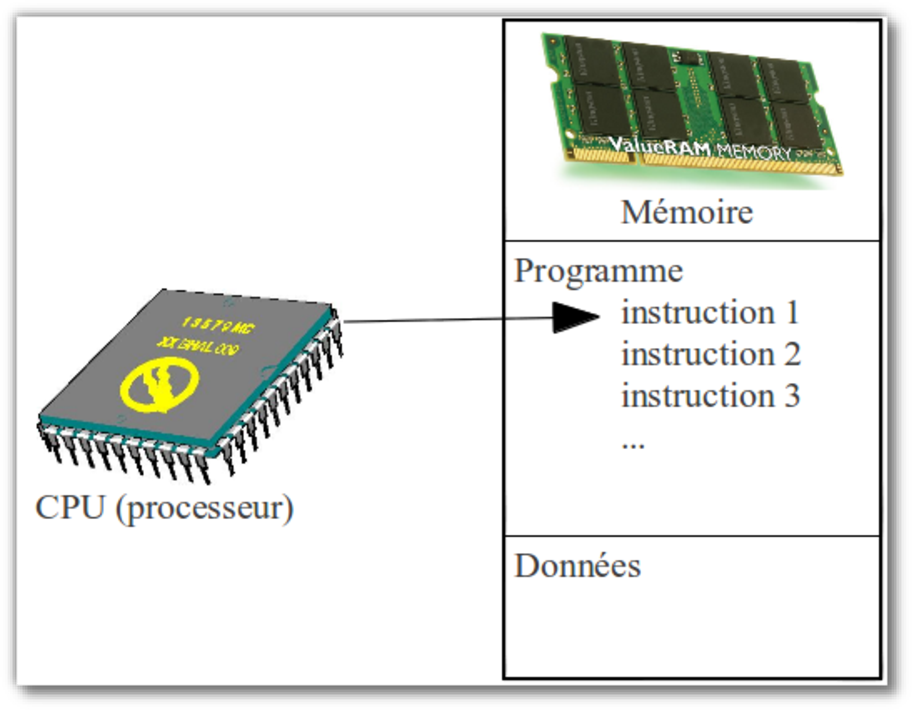
\includegraphics[width=0.45\textwidth]{image/intro-schema-ordi}
				\end{center}
			&
				\textbf{Comment fonctionne le processeur~?}
		
				De façon très simplifiée, on passe par les étapes suivantes~:
		
				\medskip
				\begin{flushleft}
				\begin{enumerate}
				\item Le processeur lit l’instruction courante.
				\item Il exécute cette instruction. Cela peut amener à manipuler les données.
				\item L’instruction suivante devient l’instruction courante.
				\item On revient au point 1.
				\end{enumerate}
				\end{flushleft}
			\\
			\end{tabular}
	
			\textbf{%
			On voit qu’il s’agit d’un travail automatique 
			ne laissant aucune place à l’initiative~!
			}
	
	%------------------------------------------------
	\section{Les phases d’élaboration d’un programme}
	%------------------------------------------------
	
		Voyons pour résumer un schéma \textbf{simplifié} des phases par
		lesquelles il faut passer quand on développe un programme.
	
		\begin{tabular}{m{0.20\linewidth}m{0.75\linewidth}}
		{\sffamily
		\begin{tikzpicture}
			\matrix [row sep = 2em] {
			 \node[draw, rounded corners, thick] (P1) {Analyse}; \\
			 \node[draw, rounded corners, thick] (P2) {Algorithmes}; \\
			 \node[draw, rounded corners, thick] (P3) {Programmation}; \\
			 \node[draw, rounded corners, thick] (P4) {Tests}; \\
			 \node[draw, rounded corners, thick] (P5) {Livraison}; \\
			};
			\draw[->, thick] (P1) to (P2);
			\draw[->, thick] (P2) to (P3);
			\draw[->, thick] (P3) to (P4);
			\draw[->, thick] (P4) to (P5);
		\end{tikzpicture}
		}
		&
		\begin{itemize}
		\item 
			Lors de \textbf{l’analyse}, 
			le problème doit être compris et clairement précisé. 
			Vous aborderez cette phase dans le cours d’analyse.
		\item
			Une fois le problème analysé, 
			et avant de passer à la phase de programmation, 
			il faut réfléchir à l’\textbf{algorithme} 
			qui va permettre de résoudre le problème. 
			C’est à cette phase précise que s’attache ce cours.
		\item
			On peut alors \textbf{programmer} cet algorithme 
			dans le langage de programmation choisi. 
			Vos cours de langage (Java, Cobol, Assembleur, \dots) 
			sont dédiés à cette phase.
		\item
			Vient ensuite la phase de \textbf{tests} 
			qui ne manquera pas de montrer qu’il subsiste des problèmes 
			qu’il faut encore corriger. 
			(Vous aurez maintes fois l’occasion 
			de vous en rendre compte lors des séances de laboratoire)
		\item
			Le produit sans bug (connu) peut être \textbf{mis en application}
			ou \textbf{livré} à la personne 
			qui vous en a passé la commande.
		\end{itemize}
		\\
		\end{tabular}
		
		Notons que ce processus n’est pas linéaire. À chaque
		phase, on pourra détecter des erreurs, imprécisions ou oublis des
		phases précédentes et revenir en arrière.
	
		\textbf{Pourquoi passer par la phase «~algorithmique~» 
			et ne pas directement passer à la programmation~?}
		
		Voilà une question que vous ne manquerez pas de vous poser 
		pendant votre apprentissage cette année. 
		Apportons quelques éléments de réflexion.
	
		\begin{itemize}
		\item
			Passer par une phase «~algorithmique~» 
			permet de séparer deux difficultés~:~
			quelle est la marche à suivre~? 
			Et comment l’exprimer dans le langage de programmation choisi~? 
			Le langage que nous allons utiliser en algorithmique 
			est plus souple et plus général que le langage Java
			par exemple (où il faut être précis au «~;~» près).
		\item
			De plus, un algorithme écrit facilite le dialogue 
			dans une équipe de développement. 
			«~J’ai écrit un algorithme 
			pour résoudre le problème qui nous occupe. 
			Qu’en pensez-vous~? Pensez-vous qu’il est correct~?
			Avez-vous une meilleure idée~?~». 
			L’algorithme est plus adapté à la communication car plus lisible.
		\item
			Enfin, si l'algorithme est écrit, 
			il pourra facilement être traduit
			dans n’importe quel langage de programmation. 
			La traduction d’un langage de programmation à un autre
			est un peu moins facile 
			à cause des particularités propres à chaque langage.
		\end{itemize}
	
		Bien sûr, cela n’a de sens que si le problème présente
		une réelle difficulté algorithmique. 
		Certains problèmes (en pratique, certaines parties de problèmes) 
		sont suffisamment simples que pour être directement programmés. 
		Mais qu’est-ce qu’un problème simple~? 
		Cela va évidemment changer tout au long de votre apprentissage. 
		Un problème qui vous paraitra difficile en début d’année 
		vous paraitra (enfin, il faut l’espérer~!) 
		une évidence en fin d’année.
	
	%-------------------
	\section{Conclusion}
	%-------------------
	
		L’informatisation de problèmes 
		est un processus essentiellement dynamique, 
		contenant des allées et venues constantes 
		entre les différentes étapes. 
		Codifier un algorithme dans un langage de programmation quelconque 
		n’est certainement pas la phase la plus difficile de ce processus. 
		Par contre, élaborer une démarche logique de résolution 
		d’un problème est probablement plus complexe.
		
		Le but du cours d'\textbf{algorithmique} est double~:
	
		\begin{itemize}
		\item
			essayer de définir une bonne démarche d’élaboration d’algorithmes
			(apprentissage de la \textbf{logique} de programmation) ;
		\item
			comprendre et apprendre les algorithmes classiques 
			qui ont fait leurs preuves.
			Pouvoir les utiliser en les adaptant 
			pour résoudre nos problèmes concrets.
		\end{itemize}
	
		Le tout devrait avoir pour résultat l’élaboration 
		de \textit{bons programmes}, 
		c’est-à-dire \textit{des programmes dont il est facile de
		se persuader qu’ils sont corrects} et des programmes dont la
		maintenance est la plus aisée possible. 
		Dans ce sens, ce cours se situe idéalement 
		en aval d’un cours d’\textbf{analyse}, 
		et en amont des cours de \textbf{langage de programmation}. 
		Ceux-ci sont idéalement complétés
		par les notions de \textbf{système d’exploitation} et de
		\textbf{persistance des données}.
	
		Afin d’envisager la résolution d’une multiplicité 
		de problèmes prenant leur source dans des domaines différents, 
		le contenu minimum de ce cours envisage l’étude des points suivants 
		(dans le désordre)~:
	
		\begin{itemize}
		\item 
			la représentation des algorithmes
		\item
			la programmation structurée
		\item
			la programmation procédurale~:~les modules et 
			le passage de paramètres
		\item
			les algorithmes de traitement des tableaux
		\item
			la résolution de problèmes récursifs
		\item
			les algorithmes liés au traitement des structures de données particulières telles
			que listes, files d’attente, piles, arbres, graphes, tables de hachage,
			etc.
		\end{itemize}
	
		Voilà bien un programme trop vaste pour un premier cours.  
		Un choix devra donc être fait et ce, en fonction
		de critères tels que la rapidité d’assimilation, l’intérêt des
		étudiants et les besoins exprimés pour des cours annexes. 
		Les matières non traitées ici, 
		le seront dans les cours d'Algorithmique II et III. 

	%-------------------
	\section{Ressources}
	%-------------------
	
		Pour prolonger votre réflexion 
		sur les notions vues dans ce chapitre, 
		nous vous proposons quelques ressources en ligne :
		\begin{itemize}
		\item
			Comment mon ordinateur \emph{réfléchit} ? 
			\url{https://www.youtube.com/watch?v=TIkBcrbzYf0}
		\end{itemize}


	\part{Les bases de l'algorithmique}
	%----------------------------------------------------------
		%==============================
\chapter{Spécifier le problème}
%==============================

	\marginicon{objectif}
	Comme nous l'avons dit, 
	un problème ne sera véritablement bien spécifié 
	que s’il s’inscrit dans le schéma suivant~:
		
	\medskip
	\begin{center}
	\begin{Ovalbox}
		{\textbf{étant donné} [les données] 
		\textbf{on demande} [résultat]}
	\end{Ovalbox}
	\end{center}
	\medskip
	
	La première étape dans la résolution d’un problème est de
	préciser ce problème à partir de l'énoncé,
	c-à-d de déterminer et préciser les données et le résultat.
	Il ne s’agit pas d’un travail facile 
	et c'est celui par lequel nous allons commencer.

	%----------------------------------------------
	\section{Déterminer les données et le résultat}
	%----------------------------------------------
	
		La toute première étape est de parvenir à extraire
		d'un énoncé de problème, quelles sont les données
		et quel est le résultat attendu%
		\footnote{%
			Plaçons-nous pour le moment dans le cadre
			de problèmes où il y a exactement un résultat.%
		}.
	
		\begin{Emphase}
			\paragraph{Exemple.}
			Soit l'énoncé suivant :
			\og
				Calculer la surface d'un rectangle 
				à partir de sa longueur et sa largeur
			\fg.
			
			Quelles sont les données ? Il y en a deux :	
			\begin{itemize}
				\item la longueur du rectangle ;
				\item sa largeur.
			\end{itemize}
		
			Quel est le résultat attendu ? la surface du rectangle.
		\end{Emphase}
		
	%----------------------------------------------
	\section{Les noms}\index{noms}
	%----------------------------------------------
	
		Pour identifier clairement chaque \textbf{donnée}
		et pouvoir y faire référence dans le futur algorithme
		nous devons lui attribuer un \textbf{nom}%		
		\footnote{%
				Dans ce cours, on va choisir des noms en Français,
				mais vous pouvez très bien choisir
				des noms Anglais si vous vous sentez
				suffisamment à l'aise avec cette langue.
		}.
		Il est important de bien choisir les noms. 
		Le but est de trouver un nom qui soit suffisamment court,
		tout en restant explicite et ne prêtant pas à confusion.
		
\clearpage
	
		\begin{Emphase}
			\paragraph{Exemple.}	
			Quel nom choisir pour la longueur d'un rectangle ?
	
			On peut envisager les noms suivants :
			\begin{itemize}
			\item
				\lda{longueur} est probablement le plus approprié.
			\item
				\lda{longueurRectangle} peut se justifier
				pour éviter toute ambigüité avec une autre longueur.
			\item
				\lda{long} peut être admis
				si le contexte permet de comprendre immédiatement
				l’abréviation.
			\item
				\lda{l} et \lda{lg} sont à proscrire car pas assez explicites.
			\item
				\lda{laLongueurDuRectangle} est inutilement long. 
			\item
				\lda{bidule} ou \lda{temp} ne sont pas de bons choix
				car ils n'ont aucun lien avec la donnée.
			\end{itemize}
		\end{Emphase}
		
		Nous allons également donner un \textbf{nom à l'algorithme}
		de résolution du problème.
		Cela permettra d'y faire référence dans les explications
		mais également de l'utiliser dans d'autres algorithmes.
		Généralement, un nom d'algorithme est :
		\begin{itemize}
		\item soit un verbe indiquant ce que fait l'algorithme ;
		\item soit un nom indiquant le résultat fourni.	
		\end{itemize}
	
		\begin{Emphase}
			\paragraph{Exemple.}	
			Quel nom choisir pour l'algorithme 
			qui calcule la surface d'un rectangle ?
	
			On peut envisager 
			le verbe \lda{calculerSurfaceRectangle}
			ou le nom \lda{surfaceRectangle} (notre préféré).
			On pourrait aussi simplifier en \lda{surface}
			s'il est évident qu'on traite des rectangles.
		\end{Emphase}
		
		Notons que les langages de programmation 
		imposent certaines limitations 
		(parfois différentes d’un langage à l’autre)
		ce qui peut nécessiter une modification du nom 
		lors de la traduction de l'algorithme en un programme.
	
	%----------------------------------------------
	\section{Les types}\index{types}
	%----------------------------------------------
		
		Nous allons également attribuer un \textbf{type} à chaque donnée
		ainsi qu'au résultat.
		Le \textbf{type} décrit la nature de son contenu,
		quelles valeurs elle peut prendre.
		
		Dans un premier temps, les seuls \textbf{types} autorisés 
		sont les suivants~:
		
		\begin{center}
		\begin{tabular}[t]{p{1.1cm}|p{12cm}}
			\raggedleft \lda{entier} & pour les nombres entiers\\
			\raggedleft \lda{réel} & pour les nombres réels\\
	%				\raggedleft \lda{caractère} & pour les différentes lettres et caractères 
	%						(par exemple ceux qui apparaissent sur un clavier~: 
	%						\lda{‘a’}, \lda{‘1’}, \lda{‘\#’}, etc.)
	%						\\
			\raggedleft \lda{chaine} & pour les chaines de caractères,
					les textes.
					(par exemple~: 
					\lda{"Bonjour"}, \lda{"Bonjour le monde !"}, 
					\lda{"a"}, \lda{""}\dots)
					\\
			\raggedleft \lda{booléen} & quand la valeur 
					ne peut être que \lda{vrai} ou \lda{faux}\\
		\end{tabular}
		\end{center}
	
		\begin{Emphase}
			\paragraph{Exemples.}	
			\begin{itemize}
			\item Pour la longueur, la largeur et la surface d'un rectangle, on prendra un réel.
			\item Pour le nom d'une personne, on choisira la chaine.
			\item Pour l'âge d'une personne, un entier est indiqué.
			\item Pour décrire si un étudiant est doubleur ou pas, un booléen est adapté.
			\item Pour représenter un mois, on préférera souvent un entier
				donnant le numéro du mois (par ex: 3 pour le mois de mars)
				plutôt qu'une chaine (par ex: "mars")
				car les manipulations, les calculs seront plus simples.
			\end{itemize}
		\end{Emphase}
	
		\subsection{Il n'y a pas d'unité}
		%-----------------------------------------
	
			Un type numérique indique que les valeurs possibles seront
			des nombres. Il n'y a là aucune notion d'unité.
			Ainsi, la longueur d'un rectangle, un réel, 
			peut valoir $2.5$ mais certainement pas $2.5 cm$.
			Si cette unité a de l'importance,
			il faut la spécifier dans le nom de la donnée ou en commentaire.
			
			\begin{Emphase}
				\paragraph{Exemple.}
				Faut-il préciser les unités 
				pour les dimensions d'un rectangle ?
				
				Si la longueur d'un rectangle vaut $6$, 
				on ne peut pas dire s'il s'agit de centimètres, 
				de mètres ou encore de kilomètres.
				Pour notre problème de calcul de la surface,
				ce n'est pas important ;
				la surface n'aura pas d'unité non plus.
				
				Si, par contre, 
				il est important de préciser que la longueur
				est donnée en centimètres,
				on pourrait l'expliciter en la nommant
				\lda{longueurCM}.	
			\end{Emphase}
	
		\subsection{Préciser les valeurs possibles}
		%-----------------------------------------
		
			Le type choisi n'est pas toujours assez précis.
			Souvent, la donnée ne pourra prendre que certaines valeurs.
			
			\begin{Emphase}
				\paragraph{Exemples.}	
				\begin{itemize} 
				\item Un âge est un entier qui ne peut pas être négatif.
				\item Un mois est un entier compris entre 1 et 12.
				\end{itemize}
			\end{Emphase}
			
			Ces précisions pourront être données en commentaire
			pour aider à mieux comprendre le problème et sa solution.
	
		\subsection{Le type des données complexes}
		%-----------------------------------------
		
			Parfois, aucun des types disponibles ne permet de représenter 
			la donnée.
			Il faut alors la décomposer.
			
			\begin{Emphase}
				\paragraph{Exemple.}	
				Quel type choisir 
				pour la date de naissance d'une personne ?
				
				On pourrait la représenter dans une chaine 
				(par ex: "17/3/1985")
				mais cela rendrait difficile le traitement, les calculs
				(par exemple, déterminer le numéro du mois).
				Le mieux est sans doute de la décomposer en trois parties : 
				le jour, le mois et l'année, tous des entiers.
			\end{Emphase}
			
			Plus loin dans le cours,
			nous verrons qu'il est possible de définir de nouveaux
			types de données grâce aux \emph{structures}%
			\footnote{
				L'orienté objet que vous verrez en Java
				le permet également et même mieux.%
			}. 
			On pourra alors définir et utiliser un type \lda{Date}
			et il ne sera plus nécessaire de décomposer une date en trois
			morceaux.
	
		\subsection{Exercice}
		%----------------------------------------------
		
			Quel(s) type(s) de données utiliseriez-vous pour représenter 
			\begin{itemize}
				\item le prix d’un produit en grande surface~?
				\item la taille de l'écran de votre ordinateur~?
				\item votre nom~?
				\item votre adresse~?
				\item le pourcentage de remise proposé pour un produit~?
				\item une date du calendrier~?
				\item un moment dans la journée~?
			\end{itemize}
			
	%----------------------------------------------
	\section{Résumé graphique}
	%----------------------------------------------
	
		Toutes les informations déjà collectées sur le problème
		peuvent être représentées graphiquement.
	
		\begin{Emphase}
			\paragraph{Exemple.}
			Pour le problème, de la surface du rectangle, 
			on fera le schéma suivant :
			
			\center\flowalgodd{longueur (réel positif)}{largeur (réel positif)}{surfaceRectangle}{réel}	
		\end{Emphase}
		
	%----------------------------------------------
	\section{Exemples numériques}
	%----------------------------------------------
	
		Une dernière étape pour vérifier que le problème
		est bien compris est de donner quelques exemples numériques.
		On peut les spécifier en français, 
		via un graphique ou via une notation compacte
		que nous allons présenter.
	
		\begin{Emphase}
			\paragraph{Exemples.}
			Voici différentes façons de présenter des exemples numériques
			pour le problème de calcul de la surface d'un rectangle :
			\begin{itemize}
			\item En français : 
				si la longueur du rectangle vaut 3 et sa largeur vaut 2, 
				alors sa surface vaut 6.			
			\item Via un schéma :	
				\begin{center}
					\flowalgodd{longueur (3)}{largeur (2)}{surfaceRectangle}{6}
				\end{center}
			\item En notation compacte :
				\lda{surfaceRectangle(3, 2)} donne $6$.
			\end{itemize}
		\end{Emphase}
	
	%----------------------------------------------
	\section{Exercices}
	%----------------------------------------------
	
		Pour les exercices suivants, 
		nous vous demandons d’imiter la démarche décrite dans ce chapitre, 
		à savoir :
		\begin{itemize}
			\item Déterminer quelles sont les données ;
				leur donner un nom et un type.
			\item Déterminer quel est le type du résultat.
			\item Déterminer un nom pertinent pour l'algorithme.
			\item Fournir un résumé graphique.
			\item Donner des exemples.
		\end{itemize}
	
		\begin{Exercice}{Somme de 2 nombres}
			Calculer la somme de deux nombres donnés.
			\paragraph{Solution.}%
			\footnote{%
				Nous allons de temps en temps 
				fournir des solutions.
				En algorithmique,
				il y a souvent \textbf{plus qu'une} solution possible.
				Ce n'est donc pas parce que vous avez trouvé autre chose
				que c'est mauvais.
				Mais il peut y avoir des solutions \textbf{meilleures}
				que d'autres; 
				n'hésitez jamais à montrer la vôtre
				à votre professeur pour avoir son avis.
			}
			Il y a ici clairement 2 données.
			Comme elles n'ont pas de rôle précis,
			on peut les appeler simplement \lda{nombre1}
			et \lda{nombre2}
			(\lda{nb1} et \lda{nb2} sont aussi de bons choix).
			L'énoncé ne dit pas si les nombres sont entiers ou pas;
			restons le plus général possible en prenant des réels.
			Le résultat sera de même type que les données.
			Le nom de l'algorithme pourrait être simplement \lda{somme}.
			Ce qui donne :
			\begin{center}
				\flowalgodd{nombre1 (réel)}{nombre2 (réel)}{somme}{réel}
			\end{center}			 
			Et voici quelques exemples numériques :			
			\begin{multicols}{2}
				\begin{itemize}
				\item \lda{somme(3, 2)} donne $5$.
				\item \lda{somme(-3, 2)} donne $-1$.
				\item \lda{somme(3, 2.5)} donne $5.5$.
				\item \lda{somme(-2.5, 2.5)} donne $0$.
				\end{itemize}
			\end{multicols}			
		\end{Exercice}
	
		\begin{Exercice}{Moyenne de 2 nombres}
			Calculer la moyenne de deux nombres donnés.
		\end{Exercice}
		
		\begin{Exercice}{Surface d’un triangle}
			Calculer la surface d’un triangle connaissant sa base et sa hauteur.
		\end{Exercice}
	
		\begin{Exercice}{Périmètre d’un cercle}
			Calculer le périmètre d’un cercle dont on donne le rayon. 
		\end{Exercice}
	
		\begin{Exercice}{Surface d’un cercle}
			Calculer la surface d’un cercle dont on donne le rayon. 
		\end{Exercice}
	
		\begin{Exercice}{TVA}
			Si on donne un prix hors TVA, il faut lui ajouter 21\% 
			pour obtenir le prix TTC. Écrire un algorithme qui permet 
			de passer du prix HTVA au prix TTC.
		\end{Exercice}
	
		\begin{Exercice}{Les intérêts}
			Calculer les intérêts reçus après 1 an pour un montant placé en 
			banque à du 2\% d’intérêt.
		\end{Exercice}
	
		\begin{Exercice}{Placement}
			Étant donné le montant d’un capital placé (en \texteuro) 
			et le taux d’intérêt annuel (en \%), 
			calculer la nouvelle valeur de ce capital après un an.
		\end{Exercice}
	
		\begin{Exercice}{Prix TTC}
			Étant donné le prix unitaire d’un produit
			(hors TVA), le taux de TVA (en \%) et la quantité de produit vendue à
			un client, calculer le prix total à payer par ce client.
		\end{Exercice}
	
		\begin{Exercice}{Durée de trajet}
			Étant donné la vitesse moyenne en \textbf{m/s}
			d’un véhicule et la distance parcourue en \textbf{km} par ce véhicule,
			calculer la durée en secondes du trajet de ce véhicule.
		\end{Exercice}
	
		\begin{Exercice}{Allure et vitesse}
			L'allure d'un coureur est le temps qu'il met pour parcourir 1 km
			(par exemple, $4'37''$).
			On voudrait calculer sa vitesse (en km/h) à partir de son allure.
			Par exemple, la vitesse d'un coureur ayant une allure de
			$4'37''$ est de $13$ km/h. 
		\end{Exercice}
	
		\begin{Exercice}{Cote moyenne}
			Étant donné les résultats (cote entière sur
			20) de trois examens passés par un étudiant (exprimés par six nombres,
			à savoir, la cote et la pondération de chaque examen), calculer 
			la moyenne globale exprimée en pourcentage.
		\end{Exercice}
	
		\begin{Exercice}{Somme des chiffres}
			Calculer la somme des chiffres
			d’un nombre entier de 3 chiffres.
		\end{Exercice}
	
		\begin{Exercice}{Conversion HMS en secondes}
			Étant donné un moment dans la journée donné
			par trois nombres, à savoir, heure, minute et seconde, calculer le
			nombre de secondes écoulées depuis minuit.
		\end{Exercice}
	
		\begin{Exercice}{Conversion secondes en heures}
			Étant donné un temps écoulé depuis minuit.
			Si on devait exprimer ce temps sous la forme
			habituelle (heure, minute et seconde),
			que vaudrait la partie "heure".
	
			Ex~:~10000 secondes donnera 2 heures.
		\end{Exercice}
	
		\begin{Exercice}{Conversion secondes en minutes}
			Étant donné un temps écoulé depuis minuit.
			Si on devait exprimer ce temps sous la forme
			habituelle (heure, minute et seconde),
			que vaudrait la partie "minute".
	
			Ex~:~10000 secondes donnera 46 minutes.
		\end{Exercice}
	
		\begin{Exercice}{Conversion secondes en secondes}
			Étant donné un temps écoulé depuis minuit.
			Si on devait exprimer ce temps sous la forme
			habituelle (heure, minute et seconde),
			que vaudrait la partie "seconde".
	
			Ex~:~10000 secondes donnera 40 secondes.
		\end{Exercice}	
		
	

		%=============================
\chapter{Premiers algorithmes}
%=============================

	\marginicon{objectif}
	Dans le chapitre précédent,
	vous avez appris à analyser un problème
	et à clairement le spécifier.
	Il est temps d'écrire des solutions.
	Pour cela, nous allons devoir trouver
	comment passer des données au résultat
	et l'exprimer dans un langage compris de tous, 
	le \emph{Langage de Description d'Algorithmes} 
	(ou \emph{LDA}).
	
	%================================================
	\section{Un problème simple}
	%================================================
	
		%===================================
		\subsection{Trouver l'algorithme}
		%=================================

			Illustrons notre propos sur l'exemple 
			qui a servi de fil conducteur
			tout au long du chapitre précédent.
			Rappelons l'énoncé et l'analyse qui en a été faite.
			
			\begin{Emphase}
				\paragraph{Problème.}
				Calculer la surface d'un rectangle 
				à partir de sa longueur et sa largeur.
			
				\paragraph{Analyse.} 
				Nous sommes arrivés à la spécification suivante :
				\begin{center}
				\flowalgodd{longueur (réel positif)}{largeur (réel positif)}{surfaceRectangle}{réel}
				\end{center}
				
				\textbf{Exemples.} 
				\begin{multicols}{2}
					\begin{itemize}
					\item \lda{surfaceRectangle(3,2)} donne $6$ ;
					\item \lda{surfaceRectangle(3.5,1)} donne $3.5$.		
					\end{itemize}
				\end{multicols}
			\end{Emphase}
			
			\paragraph{Comment résoudre ce problème ?} 
			La toute première étape est de comprendre 
			le lien entre les données et le résultat. 
			Ici, on va se baser sur la formule de la surface :
			\[
				\textrm{surface} = \textrm{longueur} * \textrm{largeur}
			\]
			La surface s'obtient donc en multipliant la longueur par la largeur%
			\footnote{%
				Trouver la bonne formule n'est pas toujours facile.
				Dans votre vie professionnelle, 
				vous devrez parfois écrire un algorithme
				pour un domaine que vous connaissez peu,
				voire pas du tout.
				Il vous faudra alors chercher de l'aide,
				demander à des experts du domaine.
				Dans ce cours,
				nous essaierons de nous concentrer sur des problèmes
				qui ne vous sont pas complètement étrangers.
			}.
			
			En LDA, la solution s'écrit :
			
			\begin{LDA}
				\Algo{surfaceRectangle}{\Par{longueur, largeur}{réel}}{réel}
					\Return longueur * largeur
				\EndAlgo
			\end{LDA}
		
			La paire \lda{\algorithmicalgo-\algorithmicend\ \algorithmicalgo}
			permet de délimiter l'algorithme.
			La première ligne est appelée 
			\textbf{l'entête}\index{entête} de l'algorithme.
			On y retrouve :
			\begin{itemize}
				\item 
					le nom de l'algorithme,
				\item 
					une déclaration des données, 
					qu’on appellera ici les \textbf{paramètres}, 
				\item 
					le type du résultat.
			\end{itemize}
		
			Les paramètres recevront des valeurs concrètes
			au \textbf{début} de l’exécution de l'algorithme. 
		
			L'instruction \lda{\algorithmicreturn}\index{retourner}
			permet d'indiquer la valeur du résultat, 
			ce que l'algorithme \emph{retourne}.
			Si on spécifie une formule, un calcul,
			c'est le résultat (on dit l'\emph{évaluation}) 
			de ce calcul qui est retourné et pas la formule.
		
			Pour indiquer le calcul à faire,
			écrivez-le, pour le moment,
			naturellement comme vous le feriez en mathématique.
			La seule différence notable est l'utilisation de \lda{*}
			pour indiquer une multiplication.
			Nous donnerons plus de détails plus loin.
	
			Pour indiquer qu'on veut \textbf{exécuter} un algorithme
			(on dit aussi \emph{appeler})
			il suffit d'indiquer son nom 
			et les valeur concrètes à donner aux paramètres.
			Ainsi, \lda{surfaceRectangle(6,3)}
			fait appel à l'algorithme correspondant
			pour calculer la surface d'un rectangle
			dont la longueur est $6$
			et la largeur est $3$.

		%===================================
		\subsection{Vérifier l'algorithme}
		\index{vérifier un algorithme}
		%=================================
		
			Lorsque vous avez terminé un exercice,
			vous le montrez à votre professeur pour qu'il
			vous dise s'il est correct ou pas.
			Fort bien !
			Mais vous pourriez trouver la réponse tout seul.
			Il vous suffit d'exécuter l'algorithme
			avec des exemples numériques et de vérifier que la réponse
			fournie est correcte.
			Votre professeur n'est indispensable que pour :
			\begin{itemize}
			\item
				vérifier qu'il fonctionne également
				dans certains cas particuliers
				auxquels il est difficile de penser quand on débute ;
			\item
				donner son avis sur la qualité de votre solution
				c-à-d essentiellement sur sa lisibilité.
				Nous y reviendrons.
			\end{itemize}
		
			Vous éprouvez souvent des difficultés à tester un algorithme
			car vous oubliez d'\textbf{éteindre votre cerveau}.
			Il faut agir comme une machine
			et exécuter \textbf{ce qui est écrit} 
			pas ce que vous pensez avoir écrit,
			ce qu'il est censé faire.
			Cela demande un peu de pratique.

			\paragraph{Exemple.} 
			Vérifions notre solution 
			pour le calcul de la surface du rectangle
			en reprenant les exemples choisis.
			
			\begin{center}
			\begin{tabular}{|c|cccc|c|}
			\hline
			test \no & longueur & largeur & réponse attendue & réponse fournie & {} \\\hline
			\hline 
			1 & 3   & 2 & 6   & 6   & {\color{ForestGreen}$\checkmark$} \\\hline
			2 & 3.5 & 1 & 3.5 & 3.5 & {\color{ForestGreen}$\checkmark$} \\\hline
			\end{tabular}
			\end{center}				
			
			\bigskip
			\marginicon{attention}
			\textbf{Attention} : 
			Dans tous les exercices qui suivront,
			chaque fois qu'on vous demandera d'écrire un algorithme,
			on attendra de vous : de spécifier le problème,
			de fournir des exemples, d'écrire l'algorithme
			et de le vérifier sur vos exemples.
			Ce n'est que si tous ces éléments sont présents
			que votre solution pourra être considérée comme complète.

		%-------------------------------------------
		\subsection{Exercices}\label{prem-ex-simple}
		%-------------------------------------------

			Les exercices suivants ont déjà été analysés 
			dans un précédent chapitre
			et des exemples numériques ont été choisis.
			Il ne vous reste plus qu'à écrire l'algorithme
			et à le vérifier pour les exemples choisis.

			Vous pouvez vous baser sur la fiche \vref{fiche:calcul-simple} 
			qui résume la résolution 
			du calcul de la surface d'un rectangle,
			depuis l'analyse de l'énoncé jusqu'à l'algorithme
			et à sa vérification.
	
			\begin{Exercice}{Somme de 2 nombres}
				Calculer la somme de deux nombres donnés.
				\paragraph{Solution.}
				Rappelons ce que nous avons obtenus 
				lors de la phase d'analyse du problème.
				\begin{center}
					\flowalgodd{nombre1 (réel)}{nombre2 (réel)}{somme}{réel}
				\end{center}
				Sommer deux nombres est un problème trivial.
				L'algorithme s'écrit simplement :			
				\begin{LDA}
					\Algo{somme}{\Par{nombre1, nombre2}{réel}}{réel}
						\Return nombre1 + nombre2
					\EndAlgo
				\end{LDA}
				Cet exercice est plutôt simple 
				et il est facile de vérifier qu'il fournit
				bien les bonnes réponses pour les exemples choisis.				
				\begin{center}
					\begin{tabular}{|c|cccc|c|}
					\hline
					test \no & nombre1 & nombre2 & réponse attendue & réponse fournie & {} \\\hline
					\hline 
					1 & 3    & 2   & 5   & 5   & {\color{ForestGreen}$\checkmark$} \\\hline
					2 & -3   & 2   & -1  & -1  & {\color{ForestGreen}$\checkmark$} \\\hline
					1 & 3    & 2.5 & 5.5 & 5.5 & {\color{ForestGreen}$\checkmark$} \\\hline
					2 & -2.5 & 2.5 & 0   & 0   & {\color{ForestGreen}$\checkmark$} \\\hline
					\end{tabular}
				\end{center}				
			\end{Exercice}
		
			\begin{Exercice}{Moyenne de 2 nombres}
				Calculer la moyenne de deux nombres donnés.
			\end{Exercice}
			
			\begin{Exercice}{Surface d’un triangle}
				Calculer la surface d’un triangle 
				connaissant sa base et sa hauteur.
			\end{Exercice}
		
			\begin{Exercice}{Périmètre d’un cercle}
				Calculer le périmètre d’un cercle dont on donne le rayon. 
			\end{Exercice}
		
			\begin{Exercice}{Surface d’un cercle}
				Calculer la surface d’un cercle dont on donne le rayon. 
			\end{Exercice}
		
			\begin{Exercice}{TVA}
				Si on donne un prix hors TVA, il faut lui ajouter 21\% 
				pour obtenir le prix TTC. Écrire un algorithme qui permet 
				de passer du prix HTVA au prix TTC.
			\end{Exercice}
		
			\begin{Exercice}{Les intérêts}
				Calculer les intérêts reçus après 1 an 
				pour un montant placé en banque à du 2\% d’intérêt.
			\end{Exercice}
		
			\begin{Exercice}{Placement}
				Étant donné le montant d’un capital placé (en \texteuro) 
				et le taux d’intérêt annuel (en \%), calculer la
				nouvelle valeur de ce capital après un an.
			\end{Exercice}
		
			\begin{Exercice}{Conversion HMS en secondes}
				Étant donné un moment dans la journée donné
				par trois nombres, à savoir, heure, minute et seconde, calculer le
				nombre de secondes écoulées depuis minuit.
			\end{Exercice}
	
			\begin{Exercice}{Prix TTC}
				Étant donné le prix unitaire d’un produit
				(hors TVA), le taux de TVA (en \%) 
				et la quantité de produit vendue à un client, 
				calculer le prix total à payer par ce client.
			\end{Exercice}
			
	%================================================
	\section{Décomposer les calculs}
	%================================================
	
		Dans les exercices de la section précédente,
		vous avez écrit quelques longues formules%
		\footnote{%
			Et ce n'est encore rien comparé à ce qui nous attend ;)%
		}.
		Pour que cela reste lisible,
		il serait bon de pouvoir \emph{décomposer}
		le calcul en étapes.
		Pour ce faire, nous devons introduire deux nouvelles notions :
		les \emph{variables locales} et \emph{l'assignation}.
		
		%-----------------------------------------
		\subsection{Les variables}\index{variable}
		%-----------------------------------------
		
			\marginicon{definition}
			Une \textbf{variable locale} (ou simplement variable)
			est une zone mémoire à laquelle on a donné un nom
			et qui contiendra des valeurs d'un type donné.
			Elles vont servir à retenir des étapes intermédiaires
			de calculs.
			\begin{itemize}
			\item
				On parle de \textbf{variable}
				car son contenu \emph{peut} changer
				pendant le déroulement de l'algorithme.
			\item
				On l'appelle \textbf{locale}
				car elle n'est connue et utilisable qu'au sein
				de l'algorithme où elle est déclarée%
				\footnote{%
					Certains langages proposent également des variables
					\emph{globales} qui sont connues dans tout un programme.
					Nous ne les utiliserons pas dans ce cours ;
					voilà pourquoi on se contentera de dire "variable".%
				}.
			\end{itemize}		
			Pour être utilisable, 
			une variable doit être \emph{déclarée}%
			\footnote{%
				Certains langages permettent 
				d'utiliser des variables sans les déclarer.
				Ce ne sera pas le cas de Java.
			}
			au début de l'algorithme. 	
			La déclaration\index{déclaration} d’une variable 
			est l’instruction qui définit son nom et son type. 
			On pourrait écrire~:
	
			\begin{LDA}
				\Stmt longueur et largeur seront les noms de deux objets destinés à recevoir
				\Stmt les longueur et largeur du rectangle, c’est-à-dire des nombres à valeurs réelles.
			\end{LDA}
			
			Mais, bien entendu, cette formulation, trop proche du
			langage parlé, serait trop floue et trop longue. 
			Dès lors, nous abrégerons par~:
	
			\begin{LDA}
				\Decl{longueur, largeur}{réels}
			\end{LDA}
			
			Pour choisir le nom d'une variable,
			les règles sont les mêmes que pour les données d'un problème.
	
		%-----------------------------------------
		\subsection{L'assignation}\index{assignation}
		%--------------------------------------------
	
			\marginicon{definition}
			L'\textbf{assignation} 
			(on dit aussi \emph{affectation interne}\index{affectation interne})
			est une instruction qui donne une valeur 
			à une variable ou la modifie.
	
			Cette instruction est probablement la plus importante
			car c'est ce qui permet de retenir les résultats 
			de calculs intermédiaires.
			
			\begin{LDA}
			\Let nomVariable \Gets expression
			\end{LDA}
				
			\marginicon{definition}
			Une \textbf{expression} 
			est un calcul faisant intervenir
			des variables, des valeurs explicites
			et des opérateurs (comme +, -, <\dots). 
			Une expression a une \textbf{valeur}.
					
			\paragraph{Exemples.}
			%------------------------------------------------
				
				Quelques assignations correctes :
				
				\begin{LDA}
					\Let denRes \Gets den1 * den2
					\Let cpt \Gets cpt + 1
					\Let moyenne \Gets (nombre1 + nombre2) / 2
					\Let test \Gets a < b \RComment pour une variable logique
					\Let maChaine \Gets "bonjour"
					\Let maChaine \Gets bonjour	\RComment comprenez-vous la différence ?
				\end{LDA}

				Et d'autres qui ne le sont pas :
			
				\begin{wrong}
					\begin{LDA}
					\Let somme + 1 \Gets 3
					\RComment somme + 1 n’est pas une variable
					\Let somme \Gets 3n
					\RComment 3n n’est ni un nom de variable correct ni une expression correcte
					\end{LDA}
				\end{wrong}
				
			\paragraph{Remarques}
			%------------------------
			
				\begin{itemize}
				\item 
					\textbf{Une assignation n'est pas une égalité, une définition}.
					\\Ainsi, l'assignation \lda{cpt \Gets cpt + 1}
					ne veut pas dire que $\textrm{cpt} = \textrm{cpt} + 1$,
					ce qui est mathématiquement faux 
					mais que la \emph{nouvelle} valeur de \lda{cpt}
					doit être calculée en ajoutant 1 à sa valeur actuelle.
					Ce calcul doit être effectué au moment 
					où on exécute cette instruction. 
				\item 
					Seules les variables déclarées peuvent être affectées.
				\item 
					Toutes les variables apparaissant dans une expression
					doivent avoir été affectées préalablement. 
					Le contraire provoquerait une erreur,
					un arrêt de l’algorithme.
				\item 
					La valeur affectée à une variable 
					doit être compatible avec son type.
					Pas question de mettre une chaine dans une variable
					booléenne.
				\end{itemize}
				
		\subsection{Tracer un algorithme}
		%--------------------------------
		
			Pour vérifier qu'un algorithme est correct,
			on sera souvent amené à le \textbf{tracer}.
			Cela consiste à suivre l'évolution des variables
			et à vérifier qu'elles contiennent bien à tout moment
			la valeur attendue.
			
			\paragraph{Exemple.} Traçons des bouts d'algorithmes.
			
			\begin{minipage}{4cm}
			\begin{LDA}[1]
				\Decl{a, b, c}{entiers}
				\Let a \Gets 12
				\Let b \Gets 5
				\Let c \Gets a - b
				\Let a \Gets a + c
				\Let b \Gets a
			\end{LDA}
			\end{minipage}
			\quad%
			\begin{minipage}{7cm}
			\begin{tabular}{|>{\centering\arraybackslash}m{1cm}|*{3}{>{\centering\arraybackslash}m{2cm}}|}
				\hline
				\verb_#_ & {a} & {b} & {c}\\
				\hline
				1 & {indéfini}             & {indéfini}             & {indéfini}             \\
				2 & {12}                   & {\color{gray}$\mid$}   & {\color{gray}$\mid$}   \\
				3 & {\color{gray}$\mid$}   & {5}                    & {\color{gray}$\mid$}   \\
				4 & {\color{gray}$\mid$}   & {\color{gray}$\mid$}   & {7}                    \\
				5 & {19}                   & {\color{gray}$\mid$}   & {\color{gray}$\mid$}   \\
				6 & {\color{gray}$\mid$}   & {19}                   & {\color{gray}$\mid$}   \\
				\hline
			\end{tabular}
			\end{minipage}

			\bigskip
			\begin{minipage}{4cm}
			\begin{LDA}[1]
				\Decl{a, b, c}{entiers}
				\Let a \Gets 12
				\Let c \Gets a - b
				\Let d \Gets c - 2
			\end{LDA}
			\end{minipage}
			\quad%
			\begin{minipage}{7cm}
			\begin{tabular}{|>{\centering\arraybackslash}m{1cm}|*{3}{>{\centering\arraybackslash}m{2cm}}|}
				\hline
				\verb_#_ & {a} & {b} & {c}\\
				\hline
				1 & {indéfini}             & {indéfini}             & {indéfini}             \\
				2 & {12}                   & {\color{gray}$\mid$}   & {\color{gray}$\mid$}   \\
				3 & {\color{gray}$\mid$}   & {\color{gray}$\mid$}   & ???                    \\
				4 & {\color{gray}$\mid$}   & {\color{gray}$\mid$}   & ???                    \\
				\hline
			\end{tabular}
			\end{minipage}
			
			\lda{c} ne peut pas être calculé car b n’a pas été initialisé;
			quant à \lda{d}, il n’est même pas déclaré~!

			\begin{Exercice}{Tracer des bouts de code}
				Suivez l'évolution des variables pour les bouts
				d'algorithmes donnés.
	
				\begin{minipage}{4cm}
				\begin{LDA}[1]
					\Decl{a, b, c}{entiers}
					\Let a \Gets 42
					\Let b \Gets 24
					\Let c \Gets a + b
					\Let c \Gets c - 1
					\Let a \Gets 2 * b
					\Let c \Gets c + 1
				\end{LDA}
				\end{minipage}
				\quad%
				\begin{minipage}{7cm}
					\begin{tabular}{|>{\centering\arraybackslash}m{1cm}|*{3}{>{\centering\arraybackslash}m{2cm}}|}
					\hline
					\verb_#_ & {a} & {b} & {c}\\
					\hline
					1 & {} & {} & {} \\
					2 & {} & {} & {} \\
					3 & {} & {} & {} \\
					4 & {} & {} & {} \\
					5 & {} & {} & {} \\
					6 & {} & {} & {} \\
					7 & {} & {} & {} \\
					\hline
					\end{tabular}
				\end{minipage}
				
				\bigskip
				\begin{minipage}{4cm}
				\begin{LDA}[1]
					\Decl{a, b, c}{entiers}
					\Let a \Gets 2
					\Let b \Gets a$^3$
					\Let c \Gets b - a$^2$
					\Let a \Gets $\sqrt{c}$
					\Let a \Gets a / a
				\end{LDA}
				\end{minipage}
				\quad%
				\begin{minipage}{7cm}
					\begin{tabular}{|>{\centering\arraybackslash}m{1cm}|*{3}{>{\centering\arraybackslash}m{2cm}}|}
					\hline
					\verb_#_ & {a} & {b} & {c}\\
					\hline
					1 & {} & {} & {} \\
					2 & {} & {} & {} \\
					3 & {} & {} & {} \\
					4 & {} & {} & {} \\
					5 & {} & {} & {} \\
					6 & {} & {} & {} \\
					\hline
					\end{tabular}
				\end{minipage}	
			\end{Exercice}
		
			\begin{Exercice}{Calcul de vitesse}
				Soit le problème suivant :
				\og
					Calculer la vitesse (en km/h) d'un véhicule 
					dont on donne la durée du parcours (en secondes) 
					et la distance parcourue (en mètres).
				\fg.
				
				Voici une solution : 
				\begin{LDA}[1]
				\Algo{vitesseKMH}{\Par{distanceM, duréeS}{réel}}{réel}
					\Decl{distanceKM, duréeH}{réel}
					\Let distanceKM \Gets 1000 * distanceM
					\Let duréeH \Gets 3600 * duréeS
					\Return $\frac{\textrm{distanceKM}}{\textrm{duréeH}}$
				\EndAlgo
				\end{LDA}

				L'algorithme, s'il est correct, devrait donner
				une vitesse de 1 km/h pour une distance de 1000 mètres
				et une durée de 3600 secondes.
				Testez cet algorithme avec cet exemple.

				\begin{center}
				\begin{tabular}{|>{\centering\arraybackslash}m{1cm}|*{5}{>{\centering\arraybackslash}m{2cm}}|}
					\hline
						\verb_#_  &  &  & & &  \\			
					\hline
						1 & & & & & \\
						2 & & & & & \\
						3 & & & & & \\
						4 & & & & & \\
						5 & & & & & \\
					\hline
				\end{tabular}
				\end{center}
				
				Si vous trouvez qu'il n'est pas correct,
				voyez ce qu'il faudrait changer pour le corriger.
			\end{Exercice}
		
		%---------------------------------------------
		\subsection{Exercices de décomposition}
		%---------------------------------------------
					
			Savoir, face à un cas concret, s'il est préférable 
			de décomposer le calcul ou pas, n'est pas toujours évident.	
			La section \vref{lisibilite}
			sur la lisibilité vous apportera des arguments
			qui permettront de trancher.
	
			Les exercices qui suivent sont suffisamment complexes
			que pour mériter une décomposition du calcul.
			Ils ont déjà été analysés dans un précédent chapitre.
			On vous demande à présent d'en rédiger une solution
			et de la tracer pour vérifier que le résultat est correct.
			Vous pouvez vous baser sur la fiche \vref{fiche:calcul-complexe}
			qui présente un exemple complet.
				
			\begin{Exercice}{Durée de trajet}
				\label{algo:durée}
				Étant donné la vitesse moyenne en \textbf{m/s}
				d’un véhicule et la distance parcourue en \textbf{km} par ce véhicule,
				calculer la durée en secondes du trajet de ce véhicule.
				
				\paragraph{Solution.}
				L'analyse du problème aboutit à :
				\begin{center}
					\flowalgodd{vitesseMS (réel positif)}{distanceKM (réel positif)}{duréeTrajet}{réel}
				\end{center}
				La formule qui lie les trois éléments est :
				\[
					\mathrm{vitesse} = \frac{\mathrm{distance}}{\mathrm{temps}}
					\qquad \mathrm{\ qu'on\ peut\ aussi\ exprimer}\qquad
					\mathrm{temps} = \frac{\mathrm{distance}}{\mathrm{vitesse}}					
				\]
				pour autant que les unités soient compatibles.
				Dans notre cas, il faut d'abord convertir
				la distance en mètres, selon la formule :
				\[
					\mathrm{vitesseM} = 1000 * \mathrm{vitesseKM}					
				\]
				Quelques exemple numériques :
				\begin{multicols}{2}
					\begin{itemize}
					\item \lda{duréeeTrajet(1, 1) donne $1000$}
					\item \lda{duréeeTrajet(0.5, 0.2) donne $400$}
					\end{itemize}
				\end{multicols}
				L'algorithme s'écrit :
				\begin{LDA}[1]
					\Algo{duréeTrajet}{\Par{vitesseMS, distanceKM}{réel}}{réel}
						\Decl{distanceM}{réel}
						\Let distanceM \Gets 1000 * distanceKM
						\Return distanceM / vitesseMS
					\EndAlgo
				\end{LDA}
				
				Vérifions l'algorithme pour \lda{duréeeTrajet(1, 1)}
				\begin{center}
				\begin{tabular}{|>{\centering\arraybackslash}m{1cm}|*{4}{>{\centering\arraybackslash}m{2cm}}|}
					\hline
						\verb_#_  & vitesseMS & distanceKM & distanceM & résultat \\			
					\hline
						1 & 1                    & 1                    & {}                   & {} \\
						2 & {\color{gray}$\mid$} & {\color{gray}$\mid$} & indéfini             & {} \\
						3 & {\color{gray}$\mid$} & {\color{gray}$\mid$} & 1000                 & {} \\
						4 & {\color{gray}$\mid$} & {\color{gray}$\mid$} & {\color{gray}$\mid$} & 1000 \\
					\hline
				\end{tabular}
				\end{center}
	
				et pour \lda{duréeeTrajet(0.5, 0.2)}
				\begin{center}
				\begin{tabular}{|>{\centering\arraybackslash}m{1cm}|*{4}{>{\centering\arraybackslash}m{2cm}}|}
					\hline
						\verb_#_  & vitesseMS & distanceKM & distanceM & résultat \\			
					\hline
					1 & 0.5                  & 0.2                  & {}                   & {} \\
					2 & {\color{gray}$\mid$} & {\color{gray}$\mid$} & indéfini             & {} \\
					3 & {\color{gray}$\mid$} & {\color{gray}$\mid$} & 200                  & {} \\
					4 & {\color{gray}$\mid$} & {\color{gray}$\mid$} & {\color{gray}$\mid$} & 400 \\
					\hline
				\end{tabular}
				\end{center}								
			\end{Exercice}

			\begin{Exercice}{Allure et vitesse}
				L'allure d'un coureur est le temps qu'il met pour parcourir 1 km
				(par exemple, $4'37''$).
				On voudrait calculer sa vitesse (en km/h) à partir de son allure.
				Par exemple, la vitesse d'un coureur ayant une allure de
				$4'37''$ est de $12,996389892$ km/h. 
			\end{Exercice}
		
			\begin{Exercice}{Cote moyenne}
				Étant donné les résultats (cote entière sur
				20) de trois examens passés par un étudiant (exprimés par six nombres,
				à savoir, la cote et la pondération de chaque examen), calculer 
				la moyenne globale exprimée en pourcentage.
			\end{Exercice}
	
	%=============================================
	\section{Quelques difficultés liées au calcul}
	%=============================================
	
		Vous êtes habitués à effectuer des calculs.
		L'expérience nous montre toutefois que certains calculs
		vous posent des difficultés.
		Soit parce que ce sont des opérations que vous utilisez peu,
		soit parce que vous n'avez pas l'habitude de les voir comme des
		calculs.
		Citons : 
		\begin{itemize}
		\item
			assigner des valeurs booléennes 
			en fonction de comparaisons ;
		\item
			manipuler les opérateurs logiques ;
		\item
			utiliser la division entière et le reste.
		\end{itemize}
		
		Examinons ces situations une à une
		en fournissant des exemples et des exercices
		pour que cela devienne naturel pour vous.
		
		%------------------------------------------------------------------------
		\subsection{Les comparaisons et les assignations de variables booléennes}
		%------------------------------------------------------------------------
		\index{comparaisons}
		
			Si je vous dis que $3+1$ est un calcul
			dont le résultat est $4$, un entier
			vous n'aurez aucun mal à me croire ; 
			cela vous parait évident.
			Ce qui l'est peut-être moins c'est que $1<3$ est aussi
			un calcul dont le résultat est un \emph{booléen},
			vrai en l’occurrence. 
			Ce résultat peut être assigné à une variable booléenne.			

			\textbf{Exemples.}
			Voici quelques assignations correctes 
			(les variables à gauche du \Gets sont des variables booléennes) :
			\begin{LDA}
				\Let positif \Gets nb>0 \RComment positif est mis à vrai si le nb est positif 
				\Let adulte \Gets âge$\ge$21 \RComment adulte est vrai si l'âge est 21 ou plus
				\Let réussi \Gets cote$\ge$10 \RComment réussi est mis à vrai si la cote est supérieure ou égale à 10
				\Let parfait \Gets nbFautes=0 \RComment c'est parfait si le nombre de fautes est 0
			\end{LDA}
		
			\begin{Exercice}{Écrire des expressions booléennes}
				Pour chacune des phrases suivantes,
				écrivez l'assignation qui lui correspond.
				\begin{itemize}
				\item 
					La variable booléenne \lda{négatif}
					doit indiquer si le nombre \lda{montant} est négatif.
				\item
					Un groupe est complet s'il contient exactement 20 personnes.
				\item
					Un algorithme est considéré comme long si le nombre de lignes
					dépasse 20.
				\item 
					Un étudiant a une \emph{grande distinction} si sa cote est
					de 18/20 ou plus.
				\end{itemize}
			\end{Exercice}

		%------------------------------------------------------------------------
		\subsection{Les opérations logiques}
		%------------------------------------------------------------------------
		\index{opérateurs logiques}\index{NON}\index{ET}\index{OU}
	
			Les opérateurs logiques agissent sur des expressions booléennes 
			(variables ou expressions à valeurs booléennes) 
			pour donner un résultat du même type.
	
			\begin{center}
			\begin{tabular}{m{15mm}|m{3cm}|m{8cm}}
			opérateur & nom & description \\
			\hline
			\raggedleft \lda{NON} & négation & vrai devient faux et inversement\\
			\raggedleft \lda{ET} & conjonction logique & vrai si les 2 conditions sont vraies\\
			\raggedleft \lda{OU} & disjonction logique & vrai si au moins une des 2 conditions est vraie\\
			\hline
			\end{tabular}
			\end{center}
			\medskip
			
			Ce qu'on peut résumer par les tableaux suivants :
			
			\begin{center}
			\begin{tabular}{|cccc|}
				\hline
				a & b & a ET b & a OU b \\
				\hline
				vrai & vrai & vrai & vrai \\\hline
				vrai & faux & faux & vrai \\\hline
				faux & vrai & faux & vrai \\\hline
				faux & faux & faux & faux \\\hline				
			\end{tabular}
			\qquad
			\begin{tabular}{|cc|}
				\hline
				a & NON a \\
				\hline
				vrai & faux \\\hline
				faux & vrai \\\hline
			\end{tabular}
			\end{center}

%\clearpage			
			On peut les utiliser 
			pour donner une valeur à une variable booléenne.
			Par exemple :
			
			\begin{small}
			\begin{multicols}{2}
				\begin{itemize}
					\item \lda{tarifPlein \Gets 18$\le$âge ET âge$<$60}
					\item \lda{distinction \Gets 16$\le$cote ET cote<18}
					\item \lda{nbA3chiffres \Gets 100$\le$nb ET nb$\le$999}
					\item \lda{tarifRéduit \Gets NON tarifPlein}
					\item \lda{tarifRéduit \Gets NON (18$\le$âge ET âge$<$60)}
					\item \lda{tarifRéduit \Gets âge$<$18 OU 60$\le$âge}
				\end{itemize}
			\end{multicols}
			\end{small}
	
			Écrire des calculs utilisant ces opérateurs n'est pas facile
			car le français nous induit souvent en erreur
			en nous poussant à utiliser un ET pour un OU et inversement
			ou bien à utiliser des raccourcis d'écriture ambigus%
			\footnote{%
				Vous noterez que le nombre de "et" et de "ou"
				dans cette phrase ne facilite pas sa compréhension ;)%
			}. 
			\\Par exemple, ne pas écrire : 
			\lda{tarifRéduit \Gets âge$<$18 OU $\ge$60}
	
			\paragraph{Loi de De Morgan.}
				Lorsqu'on a une expression complexe faisant intervenir
				des négations, on peut utiliser la \emph{Loi de De Morgan}
				pour la simplifier.
				Cette loi stipule que :
				\[
					\mathrm{NON}\ (a\ \mathrm{ET}\ b) \Leftrightarrow \mathrm{NON}\ a\ \mathrm{OU}\ \mathrm{NON}\ b
				\]
				\[
					\mathrm{NON}\ (a\ \mathrm{OU}\ b) \Leftrightarrow \mathrm{NON}\ a\ \mathrm{ET}\ \mathrm{NON}\ b
				\]
				
				Par exemple : \lda{tarifRéduit \Gets NON (18$\le$âge ET âge$<$60)}
				\\peut s'écrire aussi : \lda{tarifRéduit \Gets (NON 18$\le$âge) OU (NON âge$<$60)}
				\\ce qui se simplifie en : \lda{tarifRéduit \Gets âge$<$18 OU 60$\le$âge}
	
			\paragraph{Priorités et parenthèses.}
				Lorsqu'on écrit une expression mêlant les opérateurs logiques,
				on considère que NON est prioritaire sur ET qui l'est sur OU.
				
				Ainsi l'expression : \lda{NON a OU b ET c}
				doit se comprendre : \lda{(NON a) OU (b ET c)}.
				Vous pouvez toujours ajouter des parenthèses non nécessaires
				pour vous assurer d'être bien compris.

			\paragraph{Évaluation court-circuitée.}\label{court-circuit}
			
				Les opérateurs ET et OU sont des opérateurs court-circuités.
				Cela signifie que le calcul s'arrête dès qu'on peut être sûr
				de la réponse finale.
				En particulier, si la première partie d'un ET est fausse,
				on est sûr que le résultat sera faux quelle que soit la suite.
				Et si la première partie d'un OU est vraie 
				on est sûr que le résultat sera vrai.
				
				Pourquoi un tel comportement ?
				Cela permet de gagner du temps bien sûr,
				mais cela permet également d'éviter des erreurs d'exécution.
				 
				\textbf{Exemples.}
				\begin{LDA}
					\Let ok \Gets 1/b < 0.1
						\RComment provoque une erreur et un arrêt
						de l'algorithme si \lda{b=0}. 
					\Let ok \Gets b$\neq$0 ET 1/b < 0.1
						\RComment donne la valeur \lda{faux} à \lda{ok} 
						si \lda{b=0} (court-circuit). 
					\Let ok \Gets 1/b < 0.1 ET b$\neq$0
						\RComment provoque une erreur et un arrêt
						de l'algorithme si \lda{b=0}. 
				\end{LDA}
				
			\begin{Exercice}{Simplifier des expressions booléennes}
				Voici quelques assignations correctes du point de vue de la
				syntaxe mais contenant des lourdeurs d’écriture.
				Trouvez des expressions plus simples
				qui auront un effet équivalent.
				\begin{itemize}
					\item \lda{ok \Gets adulte = vrai}
					\item \lda{ok \Gets adulte = faux}
					\item \lda{ok \Gets etudiant = vrai ET jeune = faux}
					\item \lda{ok \Gets NON (adulte = vrai) ET NON (adulte = faux)}
					\item \lda{nbA3chiffres \Gets NON (nb$<$100 OU nb$\ge$1000)}
				\end{itemize}		
			\end{Exercice}
		
			\begin{Exercice}{Expressions logiques}
				Pour chacune des phrases suivantes,
				écrivez l'assignation qui lui correspond.
				\begin{itemize}
				\item J’irai au cinéma si le film me plait et que j’ai 20\texteuro{} en poche.
				\item Je n’irai pas au cinéma si je n’ai pas 20\texteuro{} en poche.
				\item Je brosserai le premier cours de la journée s’il commence à 8h et aussi si je n’ai pas dormi mes 8h.
				\item Pour réussir GEN1, il faut au moins 10 dans chacune des AA qui le composent (math, anglais, compta).	
				\end{itemize}
			\end{Exercice}
			
		%-------------------------------------------
		\subsection{La division entière et le reste}
		%-------------------------------------------
		\index{DIV}\index{MOD}
		\index{division entière}
		\index{modulo}
		
			\marginicon{definition}
			La \textbf{division entière} consiste à effectuer une division
			en ne gardant que la partie entière du résultat.
			Dans ce cours, nous la noterons \lda{DIV}.
			Dit autrement, \lda{a DIV b}
			indique combien de fois on peut \emph{mettre} b dans a.
			
			\begin{minipage}{2cm}
			\textbf{Exemples} :	
			\\
			\end{minipage}
			\begin{minipage}{9cm}
			\begin{multicols}{2}
			\begin{itemize}
				\item 7 DIV 2 vaut 3
				\item 8 DIV 2 vaut 4
				\item 6 DIV 6 vaut 1
				\item 6 DIV 7 vaut 0
			\end{itemize}
			\end{multicols}
			\end{minipage}
			
			\marginicon{definition}
			Le \textbf{reste} de la division entière de a par b
			est ce qui n'a pas été repris dans la division.
			On va le noter \lda{a MOD b}
			et on dira \emph{a modulo b}.
	
			Un exemple vous aidera à comprendre.	
			Imaginons qu'une classe comprend 14 étudiants
			qu'il faut réunir par 3
			dans le cadre d'un travail de groupe.
			On peut former 4 groupes 
			mais il restera 2 étudiants ne pouvant former un groupe complet.
			C'est le reste de la division de 14 par 3.
			
			\begin{minipage}{2cm}
			\textbf{Exemples} :	
			\\
			\end{minipage}
			\begin{minipage}{9cm}
			\begin{multicols}{2}
			\begin{itemize}
				\item 7 MOD 2 vaut 1
				\item 8 MOD 2 vaut 0
				\item 6 MOD 6 vaut 0
				\item 6 MOD 7 vaut 6
			\end{itemize}
			\end{multicols}
			\end{minipage}

			\begin{Exercice}{Calculs}
				Voici quelques petits calculs à compléter
				faisant intervenir la division entière et le reste.
				Par exemple : "14 DIV 3 = 4 reste 2"
				siginifie que 14 DIV 3 = 4 et 14 MOD 3 = 2.
				
				\begin{multicols}{2}
					\begin{itemize}
					\item 11 DIV 3 = \_\_\ reste\ \_\_
					\item 3 DIV 11 = \_\_\ reste\ \_\_
					\item 11 DIV \_\_ = 2\ reste\ 3
					\item \_\_ DIV 3 = 3\ reste\ 2
					\end{itemize}
				\end{multicols}
			\end{Exercice}

			\begin{Exercice}{Les prix ronds}
				Voici un algorithme qui reçoit une somme d'argent exprimée en centimes
				et qui calcule le nombre (entier) de centimes qu'il
				faudrait ajouter à la somme pour tomber sur un prix rond en euros.
				Testez-le avec des valeurs numériques. Est-il correct ?
				
				\begin{LDA}
				\Algo{versPrixRond}{\Par{prixCentimes}{entier}}{entier}
					\Return 100 - (prixCentimes MOD 100)
				\EndAlgo
				\end{LDA}
				
				\begin{center}
				\begin{tabular}{|c|c|c|c|c|}
				\hline
				test \no & prixCentimes & réponse correcte & valeur retournée & Correct ? \\\hline
				\hline 
				1 & 130 & 70 &  & \\\hline
				2 & 40  & 60 &  & \\\hline
				3 & 99  & 1  &  & \\\hline
				4 & 100 & 0  &  & \\\hline
				\end{tabular}
				\end{center}
				
			\end{Exercice}
			
			
			\subsubsection{Tester la divisibilité}
			%-------------------------------------
			
				Les deux opérateurs \lda{MOD} et \lda{DIV}
				sont-ils vraiment utiles ?
				Oui ! Ils vont servir pour tester si un nombre
				est un multiple d'un autre et pour extraire
				des chiffres d'un nombre.
				Commençons par la divisibilité.

				Imaginons qu'on veuille tester qu'un nombre est pair.
				Qu'est-ce qu'un nombre pair ? Un nombre qui est multiple de 2.
				C'est-à-dire dont le reste de la division par 2 est nul.
				
				\[
				\textrm{nb pair} 
					\quad\equiv\quad \textrm{nb divisible par 2} 
					\quad\equiv\quad \textrm{nb MOD 2 = 0} 
				\]
				
				On peut donc écrire : \lda{pair \Gets nb MOD 2 = 0}.
	
			\subsubsection{Extraire les chiffres d'un nombre}
			%------------------------------------------------
			
				Faisons une petite expérience numérique.
				\begin{center}
				\begin{tabular}{|l|r|}\hline
					calcul & résultat \\\hline
					\hline
					65536 MOD 10 & 6 \\  
					65536 MOD 100 & 36 \\  
					65536 MOD 1000 & 536 \\  
					65536 MOD 10000 & 5536 \\ 
					\hline 
				\end{tabular}
				\qquad
				\begin{tabular}{|l|l|}\hline
					calcul & résultat \\\hline
					\hline
					65536 DIV 10 & 6553 \\  
					65536 DIV 100 & 655 \\  
					65536 DIV 1000 & 65 \\  
					65536 DIV 10000 & 6 \\ 
					\hline 
				\end{tabular}
				\end{center}
			
				On voit que les DIV et MOD avec des puissances de 10
				permettent de garder les chiffres de droite (MOD)
				ou d'enlever les chiffres de droite (DIV).
				Combinés, ils permettent d'extraire n'importe quel
				chiffre d'un nombre.
				
				\textbf{Exemple} : (65536 DIV 100) MOD 10 = 5.

		%---------------------
		\subsection{Le hasard}\index{hasard}\index{aléatoire}
		%---------------------
			
			Il existe de nombreuses applications 
			qui font intervenir le hasard.
			Par exemple dans les jeux où on doit mélanger des cartes,
			lancer des dés, 
			faire apparaitre des ennemis de façon aléatoire\dots
			
			Le vrai hasard n'existe pas en algorithmique
			puisqu'il s'agit de suivre des étapes précises
			dans un ordre fixé.
			Pourtant, on peut concevoir des algorithmes
			qui \emph{simulent} le hasard%
			\footnote{%
				On parle de pseudo-hasard
				ou d'algorithmes pseudo-aléatoires.
			}.
			À partir d'un nombre donné%
			\footnote{%
				Ce nombre peut être fixé ou généré à partir
				de l'environnement 
				(par exemple, l'horloge interne).
			}
			(qu'on appelle \emph{graine} ou \emph{seed} en anglais)
			ils fournissent une suite de nombres qui \emph{ont l'air}
			aléatoires.			
			Concevoir de tels algorithmes est très compliqué
			et dépasse largement le cadre de ce cours.
			Nous allons juste supposer qu'on dispose,
			sans devoir l'écrire,
			d'un algorithme qui fournit un entier aléatoire.
			
			\begin{center}
				\flowalgod{n (entier)}{hasard}{entier (entre 1 et n)}
			\end{center}
			
			Dans nos algorithmes,
			nous pourrons donc écrire \lda{hasard(n)}
			pour obtenir un nombre entier aléatoire
			entre $1$ et $n$ inclus.
			
			\textbf{Exemple.}
			\begin{LDA}
				\LComment{Simule le lancé d'un dé}
				\Algo{dé}{}{entier}
					\Return hasard(6)
				\EndAlgo
			\end{LDA}

			Cet algorithme \lda{hasard()}
			peut être utilisé pour générer des nombres
			appartenant à d'autres intervalles.
			
			\begin{Exercice}{Chiffre aléatoire}
				Écrivez un algorithme qui donne un chiffre
				(de 0 à 9 donc) aléatoire.
			\end{Exercice}

			\begin{Exercice}{Nombre aléatoire entre min et max}
				Écrivez un algorithme
				qui donne un nombre entier aléatoire
				compris entre \lda{min} et \lda{max} inclus.
				\begin{LDA}
				\Entete{hasard}{\Par{min, max}{entiers}}{entier}
				\end{LDA}
			\end{Exercice}
			
		%---------------------
		\subsection{Exercices récapitulatifs sur les difficultés de calcul}
		%---------------------
		\label{prem-ex-cplx}
		
			Les exercices qui suivent n'ont pas tous étés déjà analysés
			et ils demandent des calculs faisant intervenir
			des divisions entières, des restes et/ou des expressions booléennes.
			Comme d'habitude, écrivez la spécification
			si ça n'a pas encore été fait,
			donnez des exemples, rédigez un algorithme
			et vérifiez-le.
		
			\begin{Exercice}{Nombre multiple de 5}
				\label{algo:mult5}
				Calculer si un nombre entier positif donné est un multiple de 5.
				\paragraph{Solution.}
				Dans ce problème,
				il y a une donnée, le nombre à tester.
				La réponse est un booléen
				qui est à vrai si le nombre donné est un multiple de 5.
				\begin{center}
				\flowalgod{nombre (entier)}{multiple5}{booléen}
				\end{center}
				\textbf{Exemples.}
				\begin{multicols}{4}
					\begin{itemize}
					\item \lda{multiple5(4)} donne faux
					\item \lda{multiple5(15)} donne vrai
					\item \lda{multiple5(0)} donne vrai
					\item \lda{multiple5(-10)} donne vrai
					\end{itemize}
				\end{multicols}
				La technique pour vérifier si un nombre est
				un multiple de 5 est de vérifier que le reste
				de la division par 5 donne 0.
				Ce qui donne :
				\begin{LDA}[1]
					\Algo{multiple5}{\Par{nombre}{entier}}{booléen}
						\Return nombre MOD 5 = 0
					\EndAlgo
				\end{LDA}
				Vérifions sur nos exemples :
				\begin{center}
				\begin{tabular}{|c|c|c|c|c|}
				\hline
				test \no & nombre & réponse correcte & valeur retournée & Correct ? \\\hline
				\hline 
				1 & 4   & faux & faux & {\color{ForestGreen}$\checkmark$} \\\hline
				2 & 15  & vrai & vrai & {\color{ForestGreen}$\checkmark$} \\\hline
				3 & 0   & vrai & vrai & {\color{ForestGreen}$\checkmark$} \\\hline
				4 & -10 & vrai & vrai & {\color{ForestGreen}$\checkmark$} \\\hline
				\end{tabular}
				\end{center}
			\end{Exercice}

\clearpage	
			\begin{Exercice}{Nombre entier positif se terminant par un 0}
				Calculer si un nombre donné se termine par un 0.
			\end{Exercice}
	
			\begin{Exercice}{Les centaines}
				Calculer la partie \emph{centaine}
				d'un nombre entier positif quelconque.
			\end{Exercice}
	
			\begin{Exercice}{Somme des chiffres}
				Calculer la somme des chiffres
				d’un nombre entier positif inférieur à 1000.
			\end{Exercice}
		
			\begin{Exercice}{Conversion secondes en heures}
				Étant donné un temps écoulé depuis minuit.
				Si on devait exprimer ce temps sous la forme
				habituelle (heure, minute et seconde),
				que vaudrait la partie "heure".
		
				Ex~:~10000 secondes donnera 2 heures.
			\end{Exercice}
		
			\begin{Exercice}{Conversion secondes en minutes}
				Étant donné un temps écoulé depuis minuit.
				Si on devait exprimer ce temps sous la forme
				habituelle (heure, minute et seconde),
				que vaudrait la partie "minute".
		
				Ex~:~10000 secondes donnera 46 minutes.
			\end{Exercice}
		
			\begin{Exercice}{Conversion secondes en secondes}
				Étant donné un temps écoulé depuis minuit.
				Si on devait exprimer ce temps sous la forme
				habituelle (heure, minute et seconde),
				que vaudrait la partie "seconde".
		
				Ex~:~10000 secondes donnera 40 secondes.
			\end{Exercice}	
		
			\begin{Exercice}{Année bissextile}
				Écrire un algorithme qui vérifie si une année est bissextile. 
				Pour rappel, les années bissextiles sont les années multiples de 4. 
				Font exception, les multiples de 100 
				(sauf les multiples de 400 qui sont bien bissextiles). 
				Ainsi $2012$ et $2400$ sont bissextiles mais pas $2010$ ni $2100$.
			\end{Exercice}

			\begin{Exercice}{Un double au dés}
				Écrire un algorithme qui simule le lancer de deux dés
				et indique s'il y a eu un double 
				(les deux dés montrant une face identique).
			\end{Exercice}
			 		 
	%===================================
	\section{Des algorithmes de qualité}
	%===================================
	
		Dans la section précédente,
		nous avons vu qu'il est possible de décomposer un calcul en étapes.
		Mais quand faut-il le faire ?	
		Ou, pour poser la question autrement :
		
			\begin{quote}
				\textbf{Puisqu'il existe plusieurs algorithmes 
				qui résolvent un problème, lequel préférer ?}
			\end{quote}
		
		Répondre à cette question, 
		c'est se demander ce qui fait la qualité d'un algorithme
		ou d'un programme informatique.
		Quels sont les critères qui permettent de juger ?
		
		C'est un vaste sujet mais nous voudrions aborder les principaux.
		
		%------------------------------------------
		\subsection{L'efficacité}\index{efficacité}
		%------------------------------------------
			
			L'\textbf{efficacité}
			désigne le fait que l'algorithme (le programme) résout%
			\footnote{%
				À ne pas confondre avec \emph{l'efficience}
				qui indique qu'il est économe en ressources.
			}
			bien le problème donné.
			C'est un minimum !
		
		%-------------------------------------------
		\subsection{La lisibilité}\index{lisibilité}
		%-------------------------------------------
		
			La \textbf{lisibilité}
			indique si une personne qui lit l'algorithme
			(ou le programme)
			peut facilement percevoir comment il fonctionne.
			C'est crucial car un algorithme (un programme) 
			est \textbf{souvent lu} par de nombreuses personnes :
			\begin{itemize}
			\item
				celles qui doivent se convaincre de sa validité
				avant de passer à la programmation ;
			\item
				celles qui doivent trouver les causes
				d'une erreur lorsque celle-ci a été rencontrée%
				\footnote{%
					On parle du processus de \emph{déverminage}
					(ou \emph{debugging} en Anglais).%
				} ;
			\item
				celles qui doivent faire évoluer l'algorithme
				ou le programme suite à une modification
				du problème ;
			\item
				et, accessoirement, celles qui doivent le coter ;)
			\end{itemize}
			
			C'est un critère \textbf{très important}
			qu'il ne faut surtout pas sous-évaluer.
			Vous en ferez d'ailleurs l'amère expérience :
			si vous négligez la lisibilité d'un algorithme,
			vous-même ne le comprendrez plus quand vous le relirez
			quelques temps plus tard !
			
			Comparer la lisibilité de deux algorithmes
			n'est pas une tâche évidente car c'est une notion subjective.
			Il faut se demander quelle version va être le plus facilement
			comprise par la majorité des lecteurs.		
			La section \vref{lisibilite}
			explique ce qui peut être fait pour rendre ses algorithmes
			plus lisibles.
				
		%---------------------------------------	
		\subsection{La rapidité}\index{rapidité}
	    %---------------------------------------
	    
			La \textbf{rapidité}
			indique si l'algorithme (le programme)
			permet d'arriver plus ou moins vite au résultat.
			
			C'est un critère qui est souvent sur-évalué, 
			essentiellement pour deux raisons.
			\begin{itemize}
				\item 
					Il est trompeur. 
					On peut croire une version plus rapide alors qu'il n'en est rien.
					Par exemple, on peut se dire que décomposer un calcul
					ralentit un programme puisqu'il doit gérer des variables
					intermédiaires.
					Ce n'est pas forcément le cas.
					Les compilateurs modernes sont capables
					de nombreuses prouesses pour optimiser le code
					et fournir un résultat aussi rapide
					qu'avec un calcul non décomposé.
				\item
					L'expérience montre que la recherche de rapidité
					mène souvent à des algorithmes moins lisibles.
					Or la lisibilité doit être privilégiée à la rapidité
					car sinon il sera impossible de corriger et/ou
					de faire évoluer l'algorithme.
			\end{itemize}
		
			Ce critère est un cas particulier de l'\emph{efficience}
			qui traite de la gestion économe des ressources.
			Nous reparlerons de rapidité
			dans le chapitre consacré à la \emph{complexité}
			des algorithmes.
		
		%---------------------	
		\subsection{La taille}
		%---------------------
		
			Nous voyons parfois des étudiants contents d'avoir
			pu écrire un algorithme en moins de lignes.
			Ce critère n'a \textbf{aucune importance} ;
			un algorithme plus court n'est pas nécessairement
			plus rapide ni plus lisible.
		
		%----------------------		
		\subsection{Conclusion}
		%----------------------		
			
			Tout ces critères n'ont pas le même poids.
			Le point le plus important est bien sûr d'écrire
			un algorithme correct mais ne vous arrêtez pas là !
			Demandez-vous s'il n'est pas possible de le re-travailler
			pour améliorer sa lisibilité%
			\footnote{%
				On appelle \emph{refactorisation}
				l'opération qui consiste à modifier
				un algorithme ou un code
				sans changer ce qu'il fait
				dans le but,
				notamment, de le rendre plus lisible.
			}.
		
	%======================
	\section{Améliorer la lisibilité d'un algorithme}\label{lisibilite}\index{lisibilite}
	%======================
		
		On vient de le voir, la lisibilité est une qualité essentielle
		que doivent avoir nos algorithmes.
		Qu'est ce qui permet d'améliorer la lisibilité d'un algorithme ?
		
		\begin{enumerate}
		\item
			Il y a d'abord la \textbf{mise en page} qui aide le lecteur
			à avoir une meilleure vue d'ensemble de l'algorithme,
			à en repérer rapidement la structure générale.
			Ainsi, dans ce syllabus :
			\begin{itemize}
			\item 
				Les mots imposés 
				(on parle de \emph{mots-clés}\index{mots-clés})
				sont mis en évidence (en gras%
				\footnote{%
					Difficile de mettre en gras avec un bic.
					Dans une version écrite vous pouvez :
					souligner le mot, le mettre en couleur ou
					l'écrire en majuscule.%
				}).
			\item
				Les instructions à l'intérieur de l'algorithme sont 
				\emph{indentées}\index{indentation}
				(décalées vers la droite).
				On indentera également les instructions
				à l'intérieur des choix et des boucles.
			\item
				Des lignes verticales relient le début et la fin
				de quelque chose. 
				Ici, un algorithme mais on pourra l'utiliser
				également pour les choix et les boucles. 
			\end{itemize}
			
			\textbf{Exemples à ne pas suivre.}
			\\
			\begin{wrong}
				\begin{LDA}
					\Entete{duréeTrajet}{\Par{vitesseMS, distanceKM}{réel}}{réel}
					\Decl{distanceM}{réel}
					\Let distanceM \Gets 1000 * distanceKM
					\Return distanceM / vitesseMS
					\Stmt \K{Fin algorithme}
				\end{LDA}
			\end{wrong}
			
			\begin{wrong}
				\begin{LDA}
					\Algo{duréeTrajet}{\Par{vitesseMS, distanceKM}{réel}}{réel}
						\Decl{distanceM}{réel}
						\Let \quad distanceM \Gets 1000 * distanceKM
						\qquad \K{return} distanceM / vitesseMS
					\EndAlgo
				\end{LDA}
			\end{wrong}
	
			Il faudra préférer
			\begin{LDA}
			\Algo{duréeTrajet}{\Par{vitesseMS, distanceKM}{réel}}{réel}
				\Decl{distanceM}{réel}
				\Let distanceM \Gets 1000 * distanceKM
				\Return distanceM / vitesseMS
			\EndAlgo
			\end{LDA}
			\medskip
		
		\item
			Il y a, ensuite, l'écriture des instructions elles-mêmes.
			Ainsi :
			\begin{itemize}
			\item
				Il faut choisir soigneusement les noms 
				(d'algorithmes, de paramètres, de variables\dots)
			\item
				Il faut décomposer (ou au contraire fusionner)
				des calculs pour arriver au résultat qu'on jugera
				le plus lisible.
			\item 
				On peut introduire des commentaires et/ou
				des constantes. 
				Deux concepts que nous allons développer maintenant.
			\end{itemize}
			
		\end{enumerate}
				
		%------------------------------------------------
		\subsection{Les commentaires}\index{commentaires}
		%------------------------------------------------
	
			\marginicon{definition}
			\textbf{Commenter} un algorithme
			signifie lui ajouter du texte explicatif
			destiné au \textbf{lecteur} pour l'aider à mieux
			comprendre le fonctionnement de l'algorithme.
			Un commentaire n'est pas utilisé par celui qui exécute
			l'algorithme; il ne modifie pas ce que l'algorithme fait.
			
			Habituellement, on distingue deux sortes de commentaires :
			\begin{itemize}
			\item
				Ceux placés \textbf{au-dessus} de l'algorithme
				qui expliquent \textbf{ce que fait} l'algorithme
				et dans quelles \textbf{conditions} il fonctionne
				(les contraintes sur les paramètres).
			\item
				Ceux placés \textbf{dans} l'algorithme
				qui expliquent \textbf{comment} il le fait.
			\end{itemize}
			
			Commenter correctement un programme
			est une tâche qui n'est pas évidente et qu'il faut travailler.
			Il faut arriver à apporter au lecteur
			une information \textbf{utile}
			qui n'apparait pas directement dans le code.
			Par exemple, il est contre-productif de répéter
			ce que l'instruction dit déjà.
			Voici quelques mauvais commentaires
			
			\begin{LDA}
				\LComment{Exemples de mauvais commentaires}
				\Decl{longueur}{réel} \RComment{La longueur est un réel}
				\Let somme \Gets 0 \RComment{On initialise la somme à 0} 
			\end{LDA}
			
			Notez qu’un excès de commentaires peut être le révélateur
			des problèmes de lisibilité du code lui-même.
			Par exemple, un choix judicieux de noms de variables 
			peut s’avérer bien plus efficace que des commentaires. 
			Ainsi, l’instruction
	
			\begin{LDA}
			\Let nouveauCapital \Gets ancienCapital * (1 + taux / 100)
			\end{LDA}
	
			dépourvue de commentaires est bien préférable aux lignes suivantes~:
	
			\begin{LDA}
			\Let c1 \Gets c0 * (1 + t / 100) \RComment calcul du nouveau capital
			\Empty \RComment c1 est le nouveau capital, c0 est l’ancien capital, t est le taux
			\end{LDA}
			
			\bigskip
			Pour résumer :
			\begin{quote}
				\bfseries
				N'hésitez pas à mettre des commentaires
				au-dessus du programme pour expliquer ce qu'il fait
				et re-travaillez votre algorithme pour que tout
				commentaire à l'intérieur de l'algorithme
				devienne superflu.
			\end{quote}

			\paragraph{Exemple.}
			Voici comment on pourrait commenter un de nos algorithmes.
			\begin{LDA}
				\LComment{Calcule la surface d'un rectangle dont on donne la largeur et la longueur.}
				\LComment{On considère que les données ne sont pas négatives.}
				\Algo{surfaceRectangle}{\Par{longueur, largeur}{réel}}{réel}
					\Return longueur * largeur
				\EndAlgo
			\end{LDA}
			
			\begin{Exercice}{Commenter la durée du trajet}
				Commentez l'algorithme qui calcule la durée d'un trajet
				(exercice \vref{algo:durée}).
			\end{Exercice}
			
		%--------------------------------------------
		\subsection{Constantes}\index{constantes}
		%--------------------------------------------
	
			Une \textbf{constante} est une information pour laquelle nom, type et
			valeur sont figés. La liste des constantes utilisées dans un algorithme
			apparaitra dans la section déclaration des variables%
			\footnote{%
				Ou en dehors des algorithmes s'il s'agit d'une
				constante universelle partagée par plusieurs algorithmes.%
			} 
			sous la forme suivante%
			\footnote{%
				L'usage est d'utiliser des noms en majuscule.%
			}~:
	
			\begin{LDA}
				\Const{PI}{3,1415}
				\Const{SEUIL\_RÉUSSITE}{12}
				\Const{ESI}{{\textquotedbl}École Supérieure d’Informatique{\textquotedbl}}
			\end{LDA}
	
			Il est inutile de spécifier leur type, celui-ci
			étant défini implicitement par la valeur de la constante.	
			L'utilisation de constantes dans vos algorithmes présente
			les avantages suivants :
			\begin{itemize}
			\item
				Une meilleure lisibilité du code,
				pour autant que vous lui trouviez un nom explicite.
			\item
				Une plus grande facilité pour modifier le code
				si la constante vient à changer 
				(modification légale du seuil de réussite par exemple).
			\end{itemize}
			
			\begin{Exercice}{Utiliser une constante}
				Trouvez un algorithme que vous avez écrit
				où l'utilisation de constante
				pourrait améliorer la lisibilité de votre solution.
			\end{Exercice}
			
	%=====================================
	\section{Interagir avec l'utilisateur}
	%=====================================
	
		Reprenons l'algorithme \lda{surfaceRectangle}
		qui nous a souvent servi d'exemple.
		Il permet de calculer la surface d'un rectangle
		dont on connait la longueur et la largeur.
		Mais d'où viennent ces données ?
		Et que faire du résultat ?
		
		Tout d'abord, un algorithme peut utiliser 
		(on dit \textbf{appeler}\index{appel}) un autre algorithme%
		\footnote{%
			Cet autre algorithme doit exister \emph{quelque part} :
			sur la même page, une autre page, un autre document,
			peu importe.
			Quand on codera cet algorithme,
			les contraintes seront plus fortes
			car il faudra que l'ordinateur
			trouve cet autre bout de code
			pour pouvoir l'exécuter.
		}.
		Pour ce faire, il doit spécifier les valeurs des paramètres ;
		il peut alors utiliser le résultat.
		L'appel s'écrit ainsi :
		
		\begin{LDA}
			\Let surface \Gets surfaceRectangle(122,3.78) \RComment{On appelle l'algorithme surfaceRectangle}
		\end{LDA}
		
		L'appel d'un algorithme est considéré comme une expression,
		un calcul qui, comme toute expression,
		possède une valeur (la valeur retournée)
		et peut intervenir dans un calcul plus grand, 
		être assignée à une variable\dots
	
		%-----------------------------------------
		\subsection{Afficher un résultat}\index{afficher}
		%-----------------------------------------
		
			Si on veut écrire un programme concret (en Java par exemple)
			qui permet de calculer des surfaces de rectangles,
			il faudra bien que ce programme communique le résultat
			à l'utilisateur du programme.
			On va l'indiquer avec la commande \lda{\K{afficher}}. 
			Ce qui donne :
			
			\begin{LDA}
				\Let surface \Gets surfaceRectangle(122,3.78)
				\Write{surface}
			\end{LDA}
	
			ou, plus simplement :
		
			\begin{LDA}
				\Write{surfaceRectangle(122,3.78)}
			\end{LDA}
	
			L'instruction \lda{\K{afficher}} signifie 
			que l'algorithme doit, à cet endroit de l'algorithme
			communiquer une information à l'utilisateur.
			La façon dont il va communiquer cette information 
			(à l'écran dans une application texte, 
			via une application graphique,
			sur un cadran de calculatrice ou de montre,
			sur une feuille de papier imprimée,
			via un synthétiseur vocal\dots)
			ne nous intéresse pas ici%
			\footnote{%
				Ce sera bien sûr une question importante
				quand il s'agira de traduire l'algorithme en un programme.%
			}.		
	
		%-----------------------------------------
		\subsection{Demander des valeurs}\index{demander}
		%-----------------------------------------
	
			Le bout d'algorithme qu'on vient d'écrire
			n'est pas encore très utile puisqu'il calcule
			toujours la surface du même rectangle.
			Il serait intéressant de demander à l'utilisateur
			ce que valent la longueur et la largeur.
			C'est le but de la commande \lda{\K{demander}}. 
	
			\begin{LDA}
				\Read{longueur}
				\Read{largeur}
				\Write{surfaceRectangle(longueur, largeur)}
			\end{LDA}
	
			L'instruction \lda{\K{demander}}
			signifie que l'utilisateur va,
			à cet endroit de l'algorithme,
			être sollicité pour donner une valeur 
			qui sera affectée à une variable.
			À nouveau, la façon dont il va indiquer cette valeur
			(au clavier dans une application texte, 
			via un champ de saisie ou une liste déroulante 
			dans une application graphique,
			via une interface tactile,
			via des boutons physiques,
			via la reconnaissance vocale\dots)
			ne nous intéresse pas ici.
	
			On peut combiner les demandes et écrire :
			
			\begin{LDA}
				\Read{longueur, largeur}
				\Write{surfaceRectangle(longueur, largeur)}
			\end{LDA}
		
		%-----------------------------------------
		\subsection{Algorithme sans paramètre}
		%-----------------------------------------
			
			Les paramètres d'un algorithme sont destinés
			aux autres algorithmes qui vont l'utiliser.
			Ils ne sont pas présents lorsque les données
			sont précisées par l'utilisateur.
			Idem pour la valeur de retour.
			Au final, on pourrait écrire :
	
			\begin{LDA}
				\Algo{TestSurface}{}{}
					\Decl{longueur, largeur}{réel}
					\Read{longueur, largeur}
					\Write{surfaceRectangle(longueur, largeur)}
				\EndAlgo
			\end{LDA}
		
			Cet algorithme n'a ni paramètre ni valeur de retour
			mais il fait appel (utilise) un autre algorithme.

		%-----------------------------------------
		\subsection{Préférer les paramètres}
		%-----------------------------------------
			
			Un algorithme avec paramètres 
			est toujours plus intéressant
			qu'un algorithme qui demande les données
			et affiche le résultat
			car il peut être utilisé (appelé) dans un autre algorithme
			pour résoudre une partie du problème.
			

		%===========================================
\chapter{Une question de choix}
%===========================================

	Vous avez déjà eu l'occasion d'aborder les alternatives
	lors de votre initiation aux algorithmes sur le site
	\url{code.org}.
	Par exemple, vous avez indiqué au zombie quelque chose comme :
	\og{}S'il existe un chemin à gauche alors tourner à gauche\fg{}.
	
	Les \textbf{alternatives}\index{alternatives} 
	permettent de n'exécuter des instructions
	que si une certaine \emph{condition} est vérifiée.
	Avec le zombie, vous testiez son environnement ;
	dans nos algorithmes, vous allez tester les données.
	
	Les algorithmes vus jusqu'à présent ne proposent
	qu'un seul \og{}chemin\fg{}, une seule \og{}histoire\fg{}.
	À chaque exécution de l'algorithme,
	les mêmes instructions s'exécutent dans le même ordres.
	Les alternatives permettent de créer des histoires différentes,
	d'adapter les instructions aux valeurs concrètes des données.
	Procédons par étapes.

%===========================================
\section{Le si}
\index{si}
%===========================================
		
	Il existe des situations où
	des instructions ne doivent pas toujours être exécutées
	et un test va nous permettre de le savoir.
	
	\paragraph{Exemple.}
	Supposons que la variable \lda{nb}
	contienne un nombre positif ou négatif,
	on ne sait pas.
	Et supposons qu'on veuille le rendre positif.
	On peut tester son signe.
	S'il est négatif on peut l'inverser.
	Par contre, s'il est positif,
	il n'y a rien à faire.
	Voici comment on peut l'écrire,
	graphiquement%
	\footnote{%
		Ce graphique, appelé 
		\emph{organigramme} ou encore \emph{ordinogramme}
		permet de représenter un algorithme
		de façon plus visuelle.
		cf. \url{http://fr.wikipedia.org/wiki/Organigramme_de_programmation}.
	} et en LDA :
	
	\qquad
	\begin{minipage}{6cm}
		\begin{tikzpicture}[node distance = 1.5cm, auto]
			\sffamily				
			\node[draw, diamond] (Test) {nb<0 ?};
			\node[draw, below of=Test] (Instr) {nb \Gets -nb};
			\node[right of=Instr] (Empty) {};		          
			\node[draw, circle, below of=Instr] (End) {};		          
			\draw[->] (Test) -- (Instr) node[near start] {Oui};
			\draw[->] (Instr) -- (End);
			\draw[->] (Test) to[out=0,in=0] node[near start] {Non}  (End);
		\end{tikzpicture}	
	\end{minipage}
	\quad
	\begin{minipage}{6cm}
		\begin{LDA}
			\If{nb<0}
				\Let nb \Gets -nb
			\EndIf
		\end{LDA}
	\end{minipage}

	La condition peut-être n'importe quelle expression (calcul)
	dont le résultat est un booléen (vrai ou faux).

	\marginicon{attention}
	Attention !
	Vous faites parfois la confusion.
	Un \og{}si\fg{} n'est pas une règle que l'ordinateur
	doit apprendre et exécuter à chaque fois que l'occasion se présente.
	La condition n'est testée que lorsqu'on arrive à cet endroit
	de l'algorithme.

	\begin{Exercice}{Compréhension}
		Tracez cet algorithme et donnez la valeur de retour.
		\begin{LDA}
		\Algo{exerciceA}{a, b~: entier}{entier}
			\Decl{c}{entier}
			\Let c \Gets 2 * a
			\If{c > b}
				\Let c \Gets c - b
			\EndIf
			\Return c
		\EndAlgo
		\end{LDA}		
		\begin{multicols}{2}
		\begin{itemize}
		\item \lda{exerciceA(2, 5)} = \_\_\_
		\item \lda{exerciceA(4, 1)} = \_\_\_
		\end{itemize}
		\end{multicols}	
	\end{Exercice}

	\begin{Exercice}{Simplification d’algorithmes}
		Voici quelques extraits d’algorithmes corrects 
		du point de vue de la syntaxe 
		mais contenant des lourdeurs d’écriture.
		Simplifiez-les.
		
		\begin{LDA}
		\If{ok = vrai}
			\Write nombre
		\EndIf
		\end{LDA}
	
		\begin{LDA}
		\If{ok = faux}
			\Write nombre
		\EndIf
		\end{LDA}
	\end{Exercice}
		
%===============================
\section{Le si-sinon}
\index{si-sinon}
%===============================
	
	Pour illustrer cette instruction,
	nous allons nous pencher sur un grand classique,
	la recherche de maximum.
	
	\paragraph{Exemple.}
	Supposons qu'on veuille déterminer
	le maximum de deux nombres,
	c'est-à-dire la plus grande des deux valeurs.
	Dans la solution, il y a deux chemins possibles.
	Le maximum devra pendre la valeur du premier nombre
	ou du second selon que le premier est plus grand 
	que le second ou pas.
	
	\qquad
	\begin{minipage}{6cm}
		\begin{tikzpicture}[node distance = 1.5cm, auto]
			\sffamily				
			\node[draw, diamond] (Test) {nb1>nb2 ?};
			\node[below of=Test] (Empty) {};
			\node[draw,left  of=Empty] (If) {max \Gets nb1};		          
			\node[draw,right  of=Empty] (Else) {max \Gets nb2};		          
			\node[draw, circle, below of=Empty] (End) {};
			\draw[->] (Test) -| (If) node[left, midway] {Oui};
			\draw[->] (If) |- (End);
			\draw[->] (Test) -| (Else) node[right, midway] {Non};
			\draw[->] (Else) |- (End);
		\end{tikzpicture}	
	\end{minipage}
	\quad
	\begin{minipage}{6cm}
		\begin{LDA}
			\If{nb1<nb2}
				\Let max \Gets nb1
			\Else
				\Let max \Gets nb2
			\EndIf
		\end{LDA}
	\end{minipage}

	\begin{Exercice}{Compréhension}
		Tracez ces algorithmes et donnez la valeur de retour.
	
		\begin{LDA}
		\Algo{exerciceB}{b, a : entier}{entier}
			\Decl{c}{entier}
			\If{a > b}
				\Let c \Gets a DIV b
			\Else
				\Let c \Gets b MOD a	
			\EndIf
			\Return c
		\EndAlgo
		\end{LDA}
	
		\begin{multicols}{2}
		\begin{itemize}
		\item \lda{exerciceB(2, 3)} = \_\_\_
		\item \lda{exerciceB(4, 1)} = \_\_\_
		\end{itemize}
		\end{multicols}
	
		\begin{LDA}
		\Algo{exerciceC}{x1, x2~: entier}{entier}
			\Decl{ok}{booléen}
			\Let ok \Gets x1 > x2
			\If{ok}
				\Let ok \Gets ok ET x1 = 4
			\Else
				\Let ok \Gets ok OU x2 = 3
			\EndIf
			\If{ok}
				\Let x1 \Gets x1 * 1000
			\EndIf
			\Return x1 + x2
		\EndAlgo
		\end{LDA}
		
		\medskip
		\begin{multicols}{2}
		\begin{itemize}
		\item \lda{exerciceC(2, 3)} = \_\_\_
		\item \lda{exerciceC(4, 1)} = \_\_\_	
		\end{itemize}
		\end{multicols}	
		
	\end{Exercice}	
	
	\begin{Exercice}{Simplification d’algorithmes}
		Voici quelques extraits d’algorithmes corrects du point de vue de la
		syntaxe mais contenant des lignes inutiles ou des lourdeurs d’écriture.
		Remplacer chacune de ces portions d’algorithme par un minimum
		d’instructions qui auront un effet équivalent.
	
		\begin{LDA}
		\If{condition}
			\Let ok \Gets vrai
		\Else
			\Let ok \Gets faux
		\EndIf
		\end{LDA}
	
		\begin{LDA}
		\If{a $>$ b}
			\Let ok \Gets faux
		\Else
			\If{a $\leq$ b}
				\Let ok \Gets vrai
			\EndIf
		\EndIf
		\end{LDA}
	\end{Exercice}

	\begin{Exercice}{Maximum de 2 nombres}
		\marginicon{java}
		Écrire un algorithme qui, étant donné deux nombres quelconques,
		recherche et retourne le plus grand des deux. Attention~! On ne veut
		pas savoir si c’est le premier ou le deuxième qui est
		le plus grand mais bien quelle est cette plus grande valeur. Le
		problème est donc bien défini même si les deux nombres sont
		identiques.
		
		\textbf{Solution.}
		Une solution complète est disponible dans la fiche \vref{fiche:max2nb}.
	\end{Exercice}
	
	\begin{Exercice}{Calcul de salaire}
		Dans une entreprise, 
		une retenue spéciale de 15\% est pratiquée 
		sur la partie du salaire mensuel qui dépasse 1200~\texteuro. 
		Écrire un algorithme qui calcule le salaire net à partir du salaire brut. 
		En quoi l’utilisation de constantes convient-elle pour améliorer cet algorithme~?
	\end{Exercice}

	\begin{Exercice}{Fonction de Syracuse}
		Écrire un algorithme qui, étant donné un entier $n$ quelconque,
		retourne le résultat de la fonction
		$f(n)=
			\left\{
			\begin{array}{rl}
				n/2 & si \ n \ est\ pair\\
				3n+1 & si \ n \ est \ impair
			\end{array}
			\right.$
	\end{Exercice}

	\begin{Exercice}{Tarif réduit ou pas}
		Dans une salle de cinéma,
		le tarif plein pour une place est de 8\texteuro{}.
		Les personnes ayant droit au tarif réduit payent 7\texteuro{}.
		Écrivez un algorithme qui reçoit un booléen
		indiquant si la personne peut bénéficier du tarif réduit
		et qui retourne le prix à payer.
	\end{Exercice}

%============================
\section{Le si-sinon-si}
\index{si-sinon-si}
%============================

	Partons à nouveau d'un exemple pour illustrer cette instruction.
	
	\begin{Emphase}
		\paragraph{Exemple.}
		On voudrait mettre dans la chaine \lda{signe}
		la valeur \lda{"positif"}, \lda{"négatif"}
		ou \lda{"nul"}
		selon qu'un nombre donné est positif, négatif ou nul.
		
		Ici, lorsqu'on va examiner le nombre, 
		trois chemins vont s'offrir à nous.

		\begin{minipage}{9cm}
			\begin{tikzpicture}[auto]
				\sffamily				
				\node[draw, diamond] (Test) {\ \ };
				\node[draw,below=1cm of Test] (nul) {signe \Gets "nul"};
				\node[draw,left=0.5cm  of nul] (pos) {signe \Gets "positif"};		          
				\node[draw,right=0.5cm  of nul] (neg) {signe \Gets "négatif"};		          
				\node[draw, circle, below=1cm of nul] (End) {};
				\draw[->] (Test) -| (pos) node[left, near end] {nb>0};
				\draw[->] (Test) -- (nul) node[midway] {nb=0};
				\draw[->] (Test) -| (neg) node[right, near end] {nb<0};
				\draw[->] (pos) |- (End);
				\draw[->] (nul) -- (End);
				\draw[->] (neg) |- (End);
 			\end{tikzpicture}	
		\end{minipage}
		\quad
		\begin{minipage}{4cm}
			\begin{LDA}
				\If{nb>0}
					\Let signe \Gets "positif"
				\ElsIf{nb=0}
					\Let signe \Gets "nul"
				\Else
					\Let signe \Gets "négatif"
				\EndIf
			\end{LDA}
		\end{minipage}
	\end{Emphase}
		
	\paragraph{Remarques.}
	\begin{itemize}
	\item
		Pour le dernier cas, on se contente
		d'un \lda{\K{sinon}} sans indiquer la condition ;
		ce serait inutile, elle serait toujours vraie.
	\item
		Le \lda{\K{si}} et le \lda{\K{si-sinon}} 
		peuvent être vus comme des cas particuliers du 
		\lda{\K{si-sinon-si}}.
	\item
		On pourrait écrire la même chose 
		avec des \lda{\K{si-sinon}} imbriqués
		mais le \lda{\K{si-sinon-si}} est plus lisible.
		\begin{LDA}
			\If{nb>0}
				\Let signe \Gets "positif"
			\Else
				\If{nb=0}
					\Let signe \Gets "nul"
				\Else
					\Let signe \Gets "négatif"
				\EndIf
			\EndIf
		\end{LDA}
		\medskip
	\item
		Lorsqu'une condition est testée,
		on sait que toutes celles au-dessus
		se sont avérées fausses.
		Cela permet parfois de simplifier la condition.
	\end{itemize}

\clearpage
	\begin{Emphase}
		\paragraph{Exemple.}
		Supposons que le prix unitaire d'un produit (\lda{prixUnitaire})
		dépende de la quantité achetée (\lda{quantité}). 
		En dessous de 10 unités, on le paie 10\texteuro{} l'unité.
		De 10 à 99 unités, on le paie 8\texteuro{} l'unité.
		À partir de 100 unités, on paie 6\texteuro{} l'unité.
		
		\begin{LDA}
			\If{quantité<10}
				\Let prixUnitaire \Gets 10
			\ElsIf{quantité<100} \Comment{On sait que ce n'est pas <10; inutile de le tester}
				\Let prixUnitaire \Gets 8
			\Else
				\Let prixUnitaire \Gets 6
			\EndIf
		\end{LDA}
		
	\end{Emphase}
			
	\begin{Exercice}{Maximum de 3 nombres}
		\marginicon{java}
		Écrire un algorithme qui, étant donnés trois nombres quelconques,
		recherche et retourne le plus grand des trois.
	\end{Exercice}
	
	\begin{Exercice}{Le signe}
		\marginicon{java}
		Écrire un algorithme qui \textbf{affiche} un message indiquant
		si un entier est strictement négatif, nul ou strictement
		positif.
	\end{Exercice}

	\begin{Exercice}{Le type de triangle}
		Écrire un algorithme qui indique si un triangle
		dont on donne les longueurs de ces 3 cotés est :
		équilatéral (tous égaux), isocèle (2 égaux)
		ou quelconque.
	\end{Exercice}

	\begin{Exercice}{Grade}
		Écrire un algorithme qui retourne le grade d'un étudiant 
		suivant la moyenne qu'il a obtenue.
		
		Un étudiant ayant obtenu 
		\begin{itemize}
			\item moins de 50\% n'a pas réussi~;
			\item de 50\% inclus à 60\% exclu a réussi~;
			\item de 60\% inclus à 70\% exclu a une satisfaction~;
			\item de 70\% inclus à 80\% exclu a une distinction~;
			\item de 80\% inclus à 90\% exclu a une grande distinction~;
			\item de 90\% inclus à 100\% inclus a la plus grande distinction.
		\end{itemize}
	\end{Exercice}

\clearpage
%=====================
\section{Le selon-que}
\index{selon-que}
%=====================

	Cette nouvelle instruction permet d'écrire plus lisiblement
	\emph{certains} \lda{\K{si-sinon-si}},
	plus précisément quand le choix d'une branche dépend
	de la valeur précise d'une variable
	(ou d'une expression).

	\begin{Emphase}
		\paragraph{Exemple.}
		Imaginons qu'une variable (\lda{numéroJour}) 
		contienne un numéro de jour de la semaine
		et qu'on veuille mettre dans une variable (\lda{nomJour})
		le nom du jour correspondant 
		("lundi" pour 1, "mardi" pour 2\dots)
		
		On peut écrire une solution avec un \lda{\K{si-sinon-si}}
		mais le \lda{\K{selon-que}} est plus lisible.

		\begin{minipage}{6cm}
			\begin{LDA}
				\If{numéroJour=1}
					\Let nomJour \Gets "lundi"
				\ElsIf{numéroJour=2}
					\Let nomJour \Gets "mardi"
				\ElsIf{numéroJour=3}
					\Let nomJour \Gets "mercredi"
				\ElsIf{numéroJour=4}
					\Let nomJour \Gets "jeudi"
				\ElsIf{numéroJour=5}
					\Let nomJour \Gets "vendredi"
				\ElsIf{numéroJour=6}
					\Let nomJour \Gets "samedi"
				\Else
					\Let nomJour \Gets "dimanche"
				\EndIf
			\end{LDA}
		\end{minipage}
		\quad
		\begin{minipage}{6cm}
			\begin{LDA}
				\Switch{numéroJour \K{vaut}}
				\Case{1} nomJour \Gets "lundi"
				\Case{2} nomJour \Gets "mardi"
				\Case{3} nomJour \Gets "mercredi"
				\Case{4} nomJour \Gets "jeudi"
				\Case{5} nomJour \Gets "vendredi"
				\Case{6} nomJour \Gets "samedi"
				\Case{7} nomJour \Gets "dimanche"
				\EndSwitch
			\end{LDA}
		\end{minipage}
		
	\end{Emphase}

	\paragraph{Remarques.}
	\begin{itemize}
	\item
		On peut spécifier plusieurs valeurs pour un cas donné.
	\item
		On peut mettre un cas \lda{\K{défaut}}
		qui sera exécuté si la valeur n'est pas reprise par ailleurs.
	\end{itemize}
	
	La syntaxe générale est :
	
	\begin{LDA}
		\Switch{expression \K{vaut}}
			\Case{liste${}_1$ de valeurs séparées par des virgules }
				\Stmt Instructions
			\Case{liste${}_2$ de valeurs séparées par des virgules }
				\Stmt Instructions
			\Empty \dots
			\Case{liste${}_k$ de valeurs séparées par des virgules }
				\Stmt Instructions
			\Case{\K{autres }}
				\Stmt Instructions
		\EndSwitch
	\end{LDA}
	
	\begin{Exercice}{Numéro du jour}
		Écrire un algorithme qui retourne le numéro de jour de la semaine
		reçu en paramètre (1 pour "lundi", 2 pour "mardi"\dots).
	\end{Exercice}
	
	\begin{Exercice}{Nombre de jours dans un mois}
		Écrire un algorithme qui retourne le nombre de jours dans un mois. 
		Le mois est lu sous forme d’un entier (1 pour janvier\dots).
		On considère dans cet exercice que le mois de février
		comprend toujours 28 jours.
	\end{Exercice}
		
\section{Exercices de synthèse}
%==============================

	Dans les exercices qui suivent,
	à vous de déterminer si une instruction de choix est nécessaire
	et laquelle est la plus adaptée.

	\begin{Exercice}{Réussir DEV1}
		Pour réussir l'UE (unité d'enseignement) GEN1,
		il faut que la cote attribuée à cette UE 
		soit supérieure ou égale à 50\%.
		Cette cote tient compte de votre examen intégré
		et de vos interrogations.
		Écrire un algorithme 
		qui reçoit la cote finale (sur 100)
		d'un étudiant pour l'UE DEV1
		et qui indique si l'étudiant à réussi cette UE.
	\end{Exercice}		

	\begin{Exercice}{Réussir GEN1}
		\label{algo:réussirGEN1}
		Pour réussir l'unité d'enseignement GEN1,
		il faut que la cote attribuée à chaque AA (activité d'apprentissage)
		soit supérieure ou égale à 50\%.
		Écrire un algorithme qui reçoit les 3 cotes (sur 20) d'AA d'un étudiant
		pour l'UE GEN1 et qui \textbf{affiche} un message
		indiquant si l'étudiant a réussi ou pas.
		S'il a réussi, l'algorithme affiche également sa moyenne
		(cherchez quelle est la pondération entre ces AA).
	\end{Exercice}		
	
	\begin{Exercice}{La fourchette}
		Écrire un algorithme qui, étant donné trois nombres, 
		retourne vrai si le premier des trois 
		appartient à l’intervalle donné par le plus petit et le plus grand 
		des deux autres (bornes exclues) et faux sinon. 
		Qu’est-ce qui change si on inclut les bornes~?
	\end{Exercice}

	\begin{Exercice}{Nombre de jours dans un mois}
		Écrire un algorithme qui donne le nombre de jours dans un mois.
		Il reçoit en paramètre le numéro du mois (1 pour janvier\dots)
		ainsi que l'année.
		Pour le mois de février, 
		il faudra répondre 28 ou 29 selon que l'année fournie
		est bissextile ou pas.
	\end{Exercice}

	\begin{Exercice}{Valider une date}
		Écrire un algorithme qui valide 
		une date donnée par trois entiers~:~ l’année, le mois et le jour.
	\end{Exercice}
	
	\begin{Exercice}{Le stationnement alternatif}
		Dans une rue où se pratique le stationnement alternatif, 
		du 1 au 15 du mois, on se gare du côté des maisons ayant un numéro impair, 
		et le reste du mois, on se gare de l’autre côté. 
		Écrire un algorithme qui, sur base de la date du jour et du numéro de maison
		devant laquelle vous vous êtes arrêté, 
		retourne vrai si vous êtes bien stationné et faux sinon.
	\end{Exercice}
	

		%===========================================
\chapter{Décomposer le problème}
\index{décomposer le code}
%===========================================

%===================
\section{Motivation}
%===================

	Jusqu'à présent, 
	les problèmes que nous avons abordés étaient relativement petits.
	Nous avons pu les résoudre avec un algorithme d'un seul tenant.
	
	Dans la réalité,
	les problèmes sont plus gros 
	et il devient nécessaire de les décomposer en sous-problèmes.
	On parle d'une \emph{approche modulaire}.
	Les avantages d'une telle décomposition sont multiples.
	\begin{itemize}
	\item
		\textbf{Cela permet de libérer l'esprit.}
		L'esprit humain ne peut pas traiter trop d'informations à la fois
		(\emph{surcharge cognitive}).
		Lorsqu'un sous-problème est résolu,
		on peut se libérer l'esprit et attaquer un autre sous-problème.
	\item
		\textbf{On peut réutiliser ce qui a été fait.}
		Si un même sous-problème apparait plusieurs fois
		dans un problème ou à travers plusieurs problèmes,
		il est plus efficace de le résoudre une fois et
		de réutiliser la solution.
	\item
		\textbf{On accroit la lisibilité.}
		Si, dans un algorithme, 
		on appelle un autre algorithme pour résoudre un sous-problème,
		le lecteur verra un nom d'algorithme qui peut être plus parlant
		que les instructions qui se cachent derrière, même s'il y en a peu.
		Par exemple, \lda{dizaine(nb)} est plus parlant que
		\lda{nb MOD 100 DIV 10} pour calculer les dizaines d'un nombre.
	\end{itemize}

	Parmis les autres avantages, 
	que vous pourrez moins percevoir en début d'apprentissage,
	citons la possibilité de répartir le travail dans une équipe.
	
%===================
\section{Exemple}
%===================

	Illustrons l’approche modulaire sur 
	le calcul du maximum de 3 nombres.

	\begin{center}
	\flowalgoddd{a (réel)}{b (réel)}{c (réel)}{max3}{réel}
	\end{center}
	
	Commençons par écrire la solution du problème plus simple~:~
	le maximum de 2 nombres.

	\begin{minipage}{6cm}
		\flowalgodd{a (réel)}{b (réel)}{max2}{réel}
	\end{minipage}
	\quad
	\begin{minipage}{7cm}
		\begin{LDA}
		\Algo{max2}{\Par{a}{réel}, \Par{b}{réel}}{réel}
			\Decl{max}{réel}
			\If{a > b}
				\Let max \Gets a
			\Else
				\Let max \Gets b
			\EndIf
			\Return max
		\EndAlgo
		\end{LDA}
	\end{minipage}
	
	Pour le maximum de 3 nombres, il existe plusieurs approches.
	Voyons celle-ci~:

	\begin{LDA}
		\Stmt 1) Calculer le maximum des deux premiers nombres, soit \lda{maxab}
		\Stmt 2) Calculer le maximum de \lda{maxab} et du troisième nombre, ce qui donne le résultat.
	\end{LDA}

	qu'on peut illustrer ainsi :
	
	\begin{center}
	\begin{tikzpicture}[auto]
		\sffamily
		\node (a) at (0,4) {a (réel)};
		\node (b) at (0,2) {b (réel)};
		\node (c) at (0,0) {c (réel)};
		\node[draw,rounded corners] (max2a) at (2,3) {max2};
		\node[draw,rounded corners] (max2b) at (4,2) {max2};
		\node (r) at (6,2) {réel};
		\draw[rounded corners] (1,0) rectangle (5,4) node[above] {max3};
		\draw[->,thick] (a) to (max2a);
		\draw[->,thick] (b) to (max2a);
		\draw[->,thick] (c) to (max2b);
		\draw[->,thick] (max2a) to (max2b);
		\draw[->,thick] (max2b) to (r);
	\end{tikzpicture}	
	\end{center}
	
	Sur base de cette idée, 
	on voit que calculer le maximum de trois nombres
	peut se faire en calculant deux fois le maximum de deux nombres.
	On ne va évidemment pas \emph{recopier}%
	\footnote{
		Cette approche serait fastidieuse,
		engendrerait de nombreuses erreurs lors du recopiage
		et serait difficile à lire.
	} dans notre solution
	ce qu'on a écrit pour le maximum de deux nombres ;
	on va plutôt y faire référence, 
	c'est-à-dire appeler l'algorithme \lda{max2}. 
	Ce qui donne :

	\begin{LDA}
	\Algo{max3}{\Par{a}{réel}, \Par{b}{réel}, \Par{c}{réel}}{réel}
		\Decl{maxab, max}{réels}
		\Let maxab \Gets max2(a,b)
		\Let max \Gets max2(maxab,c)
		\Return max
	\EndAlgo
	\end{LDA}

	qu'on peut encore simplifier en :
	
	\begin{LDA}
	\Algo{max3}{\Par{a,b,c}{réels}}{réel}
		\Return max2( max2(a,b) ,c)
	\EndAlgo
	\end{LDA}

%===================
\section{Les paramètres}
\index{paramètres}
%=======================

	Jusqu'à présent,
	nous avons considéré que les paramètres d'un algorithme (ou \emph{module}\index{module})
	correspondent à ses données et que le résultat, unique,
	est retourné.

	Il s'agit d'une situation fréquente mais pas obligatoire
	que nous pouvons généraliser.
	En pratique, on peut rencontrer trois sortes de paramètres.

	%==================================
	\subsection{Le paramètre en entrée}
	%==================================

		Le paramètre en \textbf{entrée}
		est ce que nous connaissons déjà.
		Il correspond à une donnée de l'algorithme.
		Une valeur va lui être attribuée en début d'algorithme
		et elle ne sera pas modifiée.
		On pourra faire suivre le nom du paramètre d'une flèche
		vers le bas (\In) pour rappeler son rôle.
		
		Lors de l'appel, on fournit la \textbf{valeur}
		ou, plus généralement une expression
		dont la valeur sera donnée au paramète.
		Voici un cas général de paramètre en entrée.
		
		\begin{minipage}{4cm}
			\begin{LDA}
				\LComment {Code appelant}
				\Stmt monAlgo(expr)
				\Empty
			\end{LDA}
		\end{minipage}
		\quad
		\begin{minipage}{8cm}
			\begin{LDA}
				\LComment {Code appelé}
				\Entete{monAlgo}{\Par{par\In}{entier}}{}
				\Stmt \dots
			\end{LDA}
		\end{minipage}
		
		C'est comme si l'algorithme \lda{monAlgo}
		commençait pas l'affectation
		\lda{par \Gets expr}.
		
		\textbf{Exemple.} 
		Reprenons l'exemple de \lda{max3}
		en ajoutant un petit test.

		\begin{LDA}[1]
			\Algo{test}{}{} \RComment {Code appelant}
				\Decl {max}{réel}
				\Let max \Gets max3(3, 2, 5)
				\Write max
			\EndAlgo
			\Empty
			\Algo{max3}{\Par{a\In, b\In, c\In}{réels}}{réel}
				\RComment {Code appelé}
				\Decl{maxab, max}{réels}
				\Let maxab \Gets max2(a,b)
				\Let max \Gets max2(maxab,c)
				\Return max
			\EndAlgo
		\end{LDA}

		Traçons son exécution.
		
		\begin{tabular}{|>{\centering\arraybackslash}m{1cm}
						|>{\centering\arraybackslash}m{16mm}
						|*{5}{>{\centering\arraybackslash}m{16mm}}|}
			\hline
			  & \lda{test} & \multicolumn{5}{c|}{\lda{max3}} \\
			\hline
			\# & max  & {a} & {b} & {c} & {maxab} & {max}\\
			\hline
			2    & indéfini             &                      &                      &                      &                      &          \\
			3,7  & {\color{gray}$\mid$} & 3                    & 2                    & 5                    &                      &          \\
			8    & {\color{gray}$\mid$} & {\color{gray}$\mid$} & {\color{gray}$\mid$} & {\color{gray}$\mid$} & indéfini             & indéfini \\
			9    & {\color{gray}$\mid$} & {\color{gray}$\mid$} & {\color{gray}$\mid$} & {\color{gray}$\mid$} & 3                    & indéfini \\
			10   & {\color{gray}$\mid$} & {\color{gray}$\mid$} & {\color{gray}$\mid$} & {\color{gray}$\mid$} & {\color{gray}$\mid$} & 5        \\
			11,3 & 5                    &                      &                      &                      &                      &          \\
			\hline
		\end{tabular}
		
		Note : Dans cet exemple, on trouve deux fois la variable \lda{max}.
		Il s'agit bien de deux variables \textbf{différentes} ;
		l'une est définie et connue dans \lda{test} ;
		l'autre l'est dans \lda{max3}.
		
	%==================================
	\subsection{Le paramètre en sortie}
	%==================================

		Le paramètre en \textbf{sortie}
		correspond à un résultat de l'algorithme.
		Avec la notation que nous utilisons,
		un algorithme ne peut retourner qu'une seule valeur
		ce qui est parfois une contrainte trop forte.
		Les paramètres en sortie vont permettre à l'algorithme
		de fournir plusieurs réponses.
		On fera suivre le nom du paramètre d'une flèche
		vers le haut (\Out) pour rappeler son rôle.
		Un tel paramètre n'aura pas de valeur
		au début de l'algorithme mais s'en verra attribuer une
		par l'algorithme.
		
		Lors de l'appel, on fournit une \textbf{variable}
		qui recevra la valeur finale du paramètre.
		Voici un cas général de paramètre en sortie.
		
		\begin{minipage}{4cm}
			\begin{LDA}
				\LComment {Code appelant}
				\Stmt monAlgo(variable)
				\Empty
			\end{LDA}
		\end{minipage}
		\quad
		\begin{minipage}{8cm}
			\begin{LDA}
				\LComment {Code appelé}
				\Entete{monAlgo}{\Par{par\Out}{entier}}{}
				\Stmt \dots
			\end{LDA}
		\end{minipage}

		Il n'y a \textbf{pas de \lda{\algorithmicreturn}}
		puisque les résultats sont en paramètres de sortie et pas comme
		valeur \emph{retournée}.
		C'est comme si,
		à la fin de l'algorithme appelé,
		on avait l'assignation :
		\lda{variable \Gets par}.
		
		\paragraph{Exemple.}
		On peut envisager un algorithme
		qui reçoit une durée exprimée en seconde
		et fournisse trois paramètres en sortie
		correspondant à cette même durée exprimée en heures, minutes et secondes.
		En voici le schéma et la solution :
		\begin{center}
		\flowalgorrr{totalSec (entier)}{versHMS}{heuresÉcoulées (entier)}{minutesÉcoulées (entier)}{secondesÉcoulées (entier)}
		\end{center}
			
		Voici une solution et un appel possible.
		\begin{LDA}[1]
			\Algo{versHMS}{\Par{totalSec\In, heuresÉcoulées\Out, minutesÉcoulées\Out, secondesÉcoulées\Out}{\\\hfill entiers}}{}
				\Let heuresÉcoulées \Gets totalSec DIV (60*60)
				\Let minutesÉcoulées \Gets totalSec MOD (60*60) DIV 60				
				\Let secondesÉcoulées \Gets totalSec MOD 60
			\EndAlgo
			\Empty
			\Algo{test}{}{}
				\Decl{heure,minute,seconde}{entiers}
				\Stmt versHMS(65536, heure, minute, seconde)
			\EndAlgo
		\end{LDA}
		
		Traçons-le.

		\begin{small}
		\begin{tabular}{|>{\centering\arraybackslash}m{7mm}
						|*{3}{>{\centering\arraybackslash}m{9mm}}
						|>{\centering\arraybackslash}m{10mm}
						 *{3}{>{\centering\arraybackslash}m{19mm}}
						|}
			\hline
			  & \multicolumn{3}{c|}{\lda{test}} & \multicolumn{4}{c|}{\lda{versHMS}} \\
			\hline
			\# & {\scriptsize heure} & {\scriptsize minute} & {\scriptsize seconde} & {\scriptsize totalSec} & {\scriptsize heuresEcoulées} & {\scriptsize minutesEcoulées} & {\scriptsize secondesEcoulées}\\
			\hline
			9     & indéfini & indéfini & indéfini & {} & {} & {} & {} \\
			10, 1 & {\color{gray}$\mid$} & {\color{gray}$\mid$} & {\color{gray}$\mid$} & 65536 & indéfini & indéfini & indéfini \\
			3     & {\color{gray}$\mid$} & {\color{gray}$\mid$} & {\color{gray}$\mid$} & {\color{gray}$\mid$} & 10 & {\color{gray}$\mid$} & {\color{gray}$\mid$} \\
			4     & {\color{gray}$\mid$} & {\color{gray}$\mid$} & {\color{gray}$\mid$} & {\color{gray}$\mid$} & {\color{gray}$\mid$} & 12 & {\color{gray}$\mid$} \\
			5     & {\color{gray}$\mid$} & {\color{gray}$\mid$} & {\color{gray}$\mid$} & {\color{gray}$\mid$} & {\color{gray}$\mid$} & {\color{gray}$\mid$} & 16 \\
			6, 10 & 10 & 12 & 16 &  &  &  &  \\
			\hline
		\end{tabular}
		\end{small}
				
	%==================================
	\subsection{Le paramètre en entrée-sortie}
	%==================================

		Le paramètre en \textbf{entrée-sortie}
		correspond à une situation mixte.
		Il est à la fois une donnée et un résultat de l'algorithme.
		Cela signifie que l'algorithme a pour but de le modifier.
		Un tel paramètre sera suivi d'une double flèche (\In\Out).
		
		Lors de l'appel, on fournit \textbf{une variable}.
		Sa valeur est donnée au paramètre au début de l'algorithme.
		À la fin de l'algorithme, la variable reçoit la valeur du paramètre.
		Voici un cas général de paramètre en sortie.
		
		\begin{minipage}{4cm}
			\begin{LDA}
				\LComment {Code appelant}
				\Stmt monAlgo(variable)
				\Empty
			\end{LDA}
		\end{minipage}
		\quad
		\begin{minipage}{8cm}
			\begin{LDA}
				\LComment {Code appelé}
				\Entete{monAlgo}{\Par{par\Out}{entier}}{}
				\Stmt \dots
			\end{LDA}
		\end{minipage}

		C'est comme si, dans le code appelé,
		on avait une première ligne pour donner sa valeur au paramètre
		(\lda{par \Gets variable})
		et une dernière ligne pour effectuer l'assignation opposée
		(\lda{variable \Gets par}). Il n'y a pas de \lda{\algorithmicreturn}.
				
		\paragraph{Exemple.}
		On a déjà vu un algorithme qui retourne la valeur absolue d'un nombre.
		On pourrait imaginer une variante qui \textbf{modifie}
		le nombre reçu.
		En voici le schéma et la solution avec un appel possible :

		\begin{minipage}{6cm}		
			\begin{center}
			\flowalgov{nb (réel)}{valAbsolue}
			\end{center}
		\end{minipage}
		\quad
		\begin{minipage}{6cm}		
			\begin{LDA}[1]
				\Algo{valAbsolue}{\Par{nb\In\Out}{réel}}{}
					\If{nb<0}
						\Let nb \Gets -nb
					\EndIf
				\EndAlgo
				\Empty
				\Algo{test}{}{}
				\Decl{température}{réel}
				\Let température \Gets -12.5
				\Stmt valAbsolue(température)
				\Write température
				\EndAlgo
			\end{LDA}
		\end{minipage}
		
		Traçons-le.
		
		\begin{tabular}{|>{\centering\arraybackslash}m{1cm}
						|>{\centering\arraybackslash}m{20mm}
						|*{2}{>{\centering\arraybackslash}m{20mm}}|}
			\hline
			  & \lda{test} & \multicolumn{2}{c|}{\lda{valAbsolue}} \\
			\hline
			\# & température  & nb & test \\
			\hline
			8     & indéfini &  & \\
			9     & -12.5    &  & \\
			10, 1 & {\color{gray}$\mid$} & -12.5 & \\
			2     & {\color{gray}$\mid$} & {\color{gray}$\mid$} & vrai \\
			3     & {\color{gray}$\mid$} & 12.5 & \\
			5, 10 & 12.5 &  & \\
			\hline
		\end{tabular}
		
%==================================
\section{La valeur de retour}
%==================================
	
	Une valeur de retour est toujours possible,
	mais jamais obligatoire,
	quels que soient les sortes des paramètres.
	Ainsi, on peut imaginer un algorithme
	qui possède un paramètre en sortie \textbf{et}
	qui retourne également une valeur.

	Attention !
	Un algorithme qui ne \textbf{retourne} rien (pas de \Gives)
	n'a pas de valeur ;
	il ne peut pas apparaître dans une expression
	ou être assigné à une variable.

%===================
\section{Résumons}
%===================

	Reprenons tout ce qu'on vient de voir
	avec un exemple d'algorithme qui possède tous les types de paramètres.

	\begin{LDA}
		\Algo{test}{}{}
			\Write f(pE1, pE2, pE3)
		\EndAlgo
		\Empty
		\Algo{f}{\Par{pF1\In}{entier}, \Par{pF2\Out}{entier}, \Par{pF3\In\Out}{entier}}{entier}
			\Let{\color{gray} pF1 \Gets pE1} 
			\Let{\color{gray} pF3 \Gets pE3} 
			\Empty
			\LComment Le code proprement dit de l'algorithme
			\Empty
			\Let{\color{gray} pE2 \Gets pF2} 
			\Let{\color{gray} pE3 \Gets pF3} 
			\Return réponse
		\EndAlgo
	\end{LDA}

	Pour mieux se comprendre,
	il est utile d'introduire un peu de vocabulaire.
	Les paramètres déclarés dans l'entête d'un algorithme
	sont appelés \textbf{paramètres formels}.
	Les paramètres donnés à l'appel de l'algorihtme
	sont appelés \textbf{paramètres effectifs}. 
	
	Les instructions en gris dans l'exemple ne sont pas écrites
	mais c'est comme si elles étaient présentes
	pour initialiser les paramètres formels \In{} et \InOut{}
	en début d'algorithme
	et pour donner des valeurs 
	aux paramètres effectifs \Out{} et \InOut{}
	en fin d'algorithme.
	
	On comprend pourquoi \lda{pE1} peut être une expression quelconque
	mais que \lda{pE2} et \lda{pE3} doivent être des variables,
	puisqu'elle vont recevoir une valeur.
	
	À la fin de l'algorithme, 
	c'est comme si la valeur retournée \emph{remplaçait} l'appel.
	Dans notre exemple, c'est donc cette valeur retournée
	qui sera affichée.
	
%===================
\section{Exercices}
%===================

	\begin{Exercice}{Tracer des algorithmes}
		Indiquer quels nombres sont successivement affichés 
		lors de l’exécution des algorithmes ex1, ex2, ex3 et ex4.
	
		\begin{LDA}
		\Algo{ex1}{}{}
			\Decl{x, y}{entiers}
			\Stmt addition(3, 4, x)
			\Write x
			\Let x \Gets 3
			\Let y \Gets 5
			\Stmt addition(x, y, y)
			\Write y
		\EndAlgo
		\Empty
		\Algo{addition}{a\In, b\In, c\Out~:~entiers}{}
			\Decl{somme}{entier}
			\Let somme \Gets a + b
			\Let c \Gets somme
		\EndAlgo
		\end{LDA}
	
		\begin{LDA}
		\Algo{ex2}{}{}
			\Decl{a, b}{entiers}
			\Stmt addition(3, 4, a) \Comment voir ci-dessus
			\Write a
			\Let a \Gets 3
			\Let b \Gets 5
			\Stmt addition(b, a, b)
			\Write b
		\EndAlgo
		\end{LDA}
	
		\begin{LDA}
		\Algo{ex3}{}{}
			\Decl{a, b, c}{entiers}
			\Stmt calcul(3, 4, c)
			\Write c
			\Let a \Gets 3
			\Let b \Gets 4
			\Let c \Gets 5
			\Stmt calcul(b, c, a)
			\Write a, b, c
		\EndAlgo
		\Empty
		\Algo{calcul}{a\In, b\In, c\Out~:~entiers}{}
			\Let a \Gets 2 * a
			\Let b \Gets 3 * b
			\Let c \Gets a + b
		\EndAlgo
		\end{LDA}
	
		\begin{LDA}
		\Algo{ex4}{}{}
			\Decl{a, b, c}{entiers}
			\Let a \Gets 3
			\Let b \Gets 4
			\Let c \Gets f(b)
			\Write c
			\Stmt calcul2(a, b, c)
			\Write a, b, c
		\EndAlgo
		\Empty
		\Algo{calcul2}{a\In, b\In, c\Out~:~entiers}{}
			\Let a \Gets f(a)
			\Let c \Gets 3 * b
			\Let c \Gets a + c
		\EndAlgo
		\Empty
		\Algo{f}{a\In~:~entier}{entier}
			\Decl{b}{entier}
			\Let b \Gets 2 * a + 1
			\Return b
		\EndAlgo
		\end{LDA}	
	\end{Exercice}
	
	\begin{Exercice}{Appels de module}
		Parmi les instructions suivantes (où les variables
		\lda{a}, \lda{b} et \lda{c}
		sont des entiers), lesquelles font correctement appel 
		à l'algorithme d’en-tête suivant~?
	
		\begin{LDA}
			\Entete{PGCD}{a\In,b\In~:~entiers}{entier}
		\end{LDA}
	
		\begin{LDA}
		\Stmt [1] a \Gets PGCD(24, 32)
		\Stmt [2] a \Gets PGCD(a, 24)
		\Stmt [3] b \Gets 3 * PGCD(a + b, 2*c) + 120
		\Stmt [4] PGCD(20, 30)
		\Stmt [5] a \Gets PGCD(a, b, c)
		\Stmt [6] a \Gets PGCD(a, b) + PGCD(a, c)
		\Stmt [7] a \Gets PGCD(a, PGCD(a, b))
		\Stmt [8] \K{lire} PGCD(a, b)
		\Stmt [9] \K{afficher} PGCD(a, b)
		\Stmt [10] PGCD(a, b) \Gets c
		\end{LDA}
	\end{Exercice}
	
	\begin{Exercice}{Maximum de 4 nombres}
		Écrivez un algorithme qui calcule le maximum de 4 nombres.
	\end{Exercice}

	\begin{Exercice}{Écart entre 2 durées}
		Étant donné deux durées données chacune par trois
		nombres (heure, minute, seconde),
		écrire un algorithme qui calcule
		le délai écoulé entre ces deux durées en heure(s), minute(s),
		seconde(s) sachant que la deuxième durée donnée 
		est plus petite que la première.
	\end{Exercice}
	
	\begin{Exercice}{Réussir GEN1}
		Reprenons l'exercice \vref{algo:réussirGEN1}.
		Cette fois-ci on ne veut rien afficher
		mais fournir deux résultats :
		un booléen indiquant si l'étudiant a réussi ou pas
		et un entier indiquant sa cote (qui n'a de sens que s'il a réussi). 
	\end{Exercice}

	\begin{Exercice}{Nombre de jours dans un mois}
		Écrire un algorithme qui donne le nombre de jours dans un mois.
		Il reçoit en paramètre le numéro du mois (1 pour janvier\dots)
		ainsi que l'année.
		Pour le mois de février, 
		il faudra répondre 28 ou 29 selon que l'année fournie
		est bissextile ou pas.
		Vous devez réutiliser au maximum ce que vous avez déjà fait
		lors d'exercices précédents (cf. exercice \vref{ex:bissextile}).
	\end{Exercice}

	\begin{Exercice}{Valider une date}
		Écrire un algorithme qui valide 
		une date donnée par trois entiers~:~ l’année, le mois et le jour.
		Vous devez réutiliser au maximum ce que vous avez déjà fait
		lors d'exercices précédents.
	\end{Exercice}
	
	\begin{Exercice}{Généraliser un algorithme}
		Dans l'exercice \vref{algo:mult5},
		nous avons écrit un algorithme 
		pour tester si un nombre est divisible par 5.
		Si on vous demande à présent
		un algorithme pour tester si un nombre est divisible par 3,
		vous le feriez sans peine.
		Idem pour tester la divisibilité par 2, 4, 6, 7, 8, 9\dots{}
		mais vous vous lasseriez bien vite.
		
		N'est-il pas possible d'écrire un seul algorithme,
		plus général, qui résolve tous ces problèmes d'un coup ?  
	\end{Exercice}
	

		% ============================
\chapter{Un travail répétitif}
\label{chap:bcl}
% ============================

	\marginicon{objectif}
	Les ordinateurs révèlent tout leur potentiel dans leur capacité à
	répéter inlassablement les mêmes tâches.
	Vous avez pu appréhender les boucles lors de votre initiation
	sur le site \url{code.org}.
	Voyons comment utiliser à bon escient des boucles dans nos codes.

	\marginicon{attention}
	Attention~! 
	D’expérience, nous savons que ce chapitre est difficile à appréhender. 
	Beaucoup d’entre vous perdent pied ici. 
	Accrochez-vous, faites bien tous les exercices proposés,
	montrez vos solutions à votre professeur
	et demandez de l'aide dès que vous vous sentez perdu~!

% =======================================
\section{La notion de travail répétitif}
% =======================================

	Si on veut faire effectuer un travail répétitif, 
	il faut indiquer deux choses~:
	\begin{itemize}
	\item le travail à répéter ;
	\item une indication qui permet de savoir quand s'arrêter.
	\end{itemize}

	Examinons quelques exemples pour fixer notre propos.

	\paragraph{Exemple 1.} 
	Pour traiter des dossiers, 
	on dira quelque chose comme 
	«~tant qu’il reste un dossier à traiter, le traiter~» 
	ou encore 
	«~traiter un dossier puis passer au suivant jusqu’à ce qu’il n’en reste plus à traiter~».
	\begin{itemize}
	\item La tâche à répéter est : «~traiter un dossier~».
	\item On indique qu’on doit continuer s’il reste encore un dossier à traiter.
	\end{itemize}

	\paragraph{Exemple 2.}
	Pour calculer la cote finale de tous les étudiants,
	on aura quelque chose du genre 
	«~Pour tout étudiant, calculer sa cote~».
	\begin{itemize}
	\item 
		La tâche à répéter est : «~calculer la cote d’un étudiant~».
	\item 
		On indique qu’on doit le faire pour tous les étudiants.
		On doit donc commencer par le premier, passer à chaque fois au suivant
		et s’arrêter quand on a fini le dernier.
	\end{itemize}

	\paragraph{Exemple 3.}
	Pour afficher tous les nombres de 1 à 100, on aura
	«~Pour tous les nombres de 1 à 100, afficher ce nombre~».
	\begin{itemize}
	\item
		La tâche à répéter est : «~afficher un nombre~».
	\item 
		On indique qu’on doit le faire pour tous les nombres de 1 à 100. 
		On doit donc commencer avec 1, 
		passer à chaque fois au nombre suivant 
		et s’arrêter après avoir affiché le nombre 100.
	\end{itemize}
		
% ===================================================
\section{Une même instruction, des effets différents}
% ===================================================

	Comprenez bien que c’est toujours la même tâche qui est exécutée 
	mais pas avec le même effet à chaque fois. 
	Ainsi, on traite un dossier mais à chaque fois un différent ; 
	on affiche un nombre mais à chaque fois un différent. 
	
	Par exemple, la tâche à répéter pour afficher des nombres
	ne peut pas être
	\lda{\K{afficher} 1} ni \lda{\K{afficher} 2} ni\dots{}
	Par contre, on pourra utiliser l'instruction
	\lda{\K{afficher} nb} si on s'arrange pour que la variable
	\lda{nb} s'adapte à chaque passage dans la boucle.

	\begin{quote}
		\bfseries
		De façon générale,
		pour obtenir un travail répétitif,
		il faut trouver une formulation de la tâche
		qui va produire un effet différent à chaque fois.
	\end{quote}
	
	\subsection{Exemple - Afficher les nombres de 1 à 5}
	%===================================================
	
		Si on veut un algorithme qui affiche les nombres de 1 à 5
		sans utiliser de boucle, on pourrait écrire :
		
		\begin{LDA}
		\Write{1}
		\Write{2}
		\Write{3}
		\Write{4}
		\Write{5}
		\end{LDA}
		
		Ces cinq instructions sont proches mais pas tout-à-fait identiques. 
		En l'état, on ne peut pas encore en faire une boucle%
		\footnote{%
			Vous vous dites peut-être que ce code est simple ;
			inutile d'en faire une boucle.
			Ce n'est qu'un exemple.
			Que feriez-vous s'il faillait afficher les nombres
			de 1 à 1000 ?
		} ;
		il va falloir ruser.
		On peut obtenir le même résultat avec l'algorithme suivant :

		\begin{minipage}{4cm}
		\begin{LDA}
		\Let nb \Gets 1
		\Write{nb}
		\Let nb \Gets 2
		\Write{nb}
		\Let nb \Gets 3
		\Write{nb}
		\Let nb \Gets 4
		\Write{nb}
		\Let nb \Gets 5
		\Write{nb}
		\end{LDA}
		\end{minipage}
		\quad ou encore \quad
		\begin{minipage}{4cm}
		\begin{LDA}[1]
		\Let nb \Gets 1
		\Write{nb}
		\Let nb \Gets nb + 1
		\Write{nb}
		\Let nb \Gets nb + 1
		\Write{nb}
		\Let nb \Gets nb + 1
		\Write{nb}
		\Let nb \Gets nb + 1
		\Write{nb}
		\Let nb \Gets nb + 1
		\end{LDA}
		\end{minipage}
		
		Il est plus compliqué,
		mais cette fois les lignes 2 et 3 se répètent exactement.
		D'ailleurs, la dernière ligne ne sert à rien d'autre qu'à
		obtenir cinq copies identiques.
		Le travail à répéter est donc :

		\begin{LDA}
		\Write{nb}
		\Let nb \Gets nb + 1
		\end{LDA}

		Cette tâche doit être effectuée cinq fois dans notre exemple.
		Il existe plusieurs structures répétitives
		qui vont se distinguer par la façon dont on va
		contrôler le nombre de répétitions.
		Voyons-les une à une%
		\footnote{%
			Nous ne verrons pas de structure de type
			\lda{répéter 5 fois\dots}
			Elle est simple à comprendre
			mais pas souvent adaptée au problème à résoudre.
		}.

\clearpage
%========================
\section{«~tant que~»}\index{tant que}
%========================
	
	\begin{wrapfigure}{r}{6cm}
		\begin{tikzpicture}[>=triangle 60, node distance = 1.5cm, auto]
			\sffamily				
			\node[draw, diamond, aspect=2] (Test) {condition vraie ?};
			\node[draw, below of=Test] (Instr) {instructions à exécuter};
			\node[draw, circle, below of=Instr] (End) {};		          
			\draw[->] (Test) -- (Instr) node[near start] {Oui};
			\draw[->] (Test.east) to[in=0,out=0] node[near start] {Non} (End.east);
			\draw[->] (Instr.west) to[bend left] (Test.west);
		\end{tikzpicture}	
		\vspace{-1cm}
	\end{wrapfigure}
	Le «~tant que~» est une structure qui demande à
	l’exécutant de répéter une tâche (une ou plusieurs
	instructions) tant qu’une condition donnée est vraie.

	\begin{LDA}
	\While{condition}
		\Stmt séquence d’instructions à exécuter
	\EndWhile
	\end{LDA}

	Comme pour la structure \lda{si}, 
	la \lda{condition} est une expression à valeur booléenne. 
	Dans ce type de structure, 
	il faut qu’il y ait dans la séquence d’instructions comprise entre
	\lda{tant que} et \lda{fin tant que} au moins une
	instruction qui modifie une des composantes de la condition de telle
	manière qu’elle puisse devenir \textbf{fausse} à un moment donné. Dans
	le cas contraire, la condition reste indéfiniment vraie et la boucle va
	tourner sans fin, c’est ce qu’on appelle une \textbf{boucle infinie}. 
	L'ordinogramme ci-dessus décrit  le déroulement de cette structure. 
	On remarquera que si la condition est fausse dès le début, 
	la tâche n’est jamais exécutée.


	\subsection{Exemple - Afficher les nombres de 1 à 5}
	%===================================================

		Reprenons notre exemple d'affichage des nombres de 1 à 5.
		Pour rappel, la tâche à répéter est :

		\begin{LDA}
		\Write{nb}
		\Let nb \Gets nb + 1
		\end{LDA}
		
		La condition va se baser sur la valeur de \lda{nb}.
		On continue tant que le nombre n'a pas dépassé 5.
		Ce qui donne (en n'oubliant pas l'initialisation de \lda{nb}) :

		\begin{minipage}{5cm}
			\begin{LDA}[1]
				\Algo{compteur5}{}{}
					\Decl{nb}{entier}
					\Let nb \Gets 1
					\While{nb $\le$ 5}
						\Write{nb}
						\Let nb \Gets nb + 1
					\EndWhile
				\EndAlgo
			\end{LDA}
		\end{minipage}
		\quad
		\begin{minipage}{8cm}
			\begin{tabular}{|>{\centering\arraybackslash}m{6mm}
						|*{3}{>{\centering\arraybackslash}m{2cm}}|}
				\hline
					\verb_#_  & nb & condition & affichage \\			
				\hline
					2 & indéfini & {} & {} \\
					3 & 1                    & {}   & {} \\
					4 & {\color{gray}$\mid$} & vrai & {} \\
					5 & {\color{gray}$\mid$} &      & 1  \\
					6 & 2                    & {}   & {} \\
					4 & {\color{gray}$\mid$} & vrai & {} \\
					5 & {\color{gray}$\mid$} &      & 2  \\
					6 & 3                    & {}   & {} \\
					4 & {\color{gray}$\mid$} & vrai & {} \\
					5 & {\color{gray}$\mid$} &      & 3  \\
					6 & 4                    & {}   & {} \\
					4 & {\color{gray}$\mid$} & vrai & {} \\
					5 & {\color{gray}$\mid$} &      & 4  \\
					6 & 5                    & {}   & {} \\
					4 & {\color{gray}$\mid$} & vrai & {} \\
					5 & {\color{gray}$\mid$} &      & 5  \\
					6 & 6                    & {}   & {} \\
					4 & {\color{gray}$\mid$} & faux & {} \\
				\hline
			\end{tabular}
		\end{minipage}

	\subsection{Exemple - Généralisation à n nombres}
	%===================================================

		On peut généraliser l'exemple précédent
		en affichant tous les nombres de 1 à n où n est une donnée
		de l'algorithme.
		
		\begin{LDA}
		\Algo{compteur}{\Par{n}{entier}}{}
			\Decl{nb}{entier}
			\Let nb \Gets 1
			\While{nb $\le$ n}
				\Write{nb}
				\Let nb \Gets nb + 1
			\EndWhile
		\EndAlgo
		\end{LDA}

	\subsection{Exercices}
	% =====================================

		\begin{Exercice}{Compréhension d’algorithmes}
			Quels sont les affichages réalisés lors de l’exécution
			des algorithmes suivants~?
			
			\begin{minipage}[t]{40mm}
				\begin{LDA}
				\Algo{boucle1}{}{}
					\Decl{x}{entier}
					\Let x \Gets 0
					\While{x < 12}
						\Let x \Gets x + 2	
					\EndWhile
					\Write x
				\EndAlgo
				\end{LDA}
			\end{minipage}
			\ 
			\begin{minipage}[t]{45mm}
				\begin{LDA}
				\Algo{boucle2}{}{}
					\Decl{ok}{booléen}
					\Decl x : entier
					\Let ok \Gets vrai
					\Let x \Gets 5
					\While{ok}
						\Let x \Gets x + 7	
						\Let ok \Gets x MOD 11 $\neq$ 0	
					\EndWhile
					\Write x
				\EndAlgo
				\end{LDA}
			\end{minipage}
			\ 
			\begin{minipage}[t]{50mm}
				\begin{LDA}
				\Algo{boucle3}{}{}
					\Decl{ok}{booléen}
					\Decl cpt, x : entiers
					\Let x \Gets 10
					\Let cpt \Gets 0
					\Let ok \Gets vrai
					\While{ok ET cpt < 3}
						\If{x MOD 2 = 0}
							\Let x \Gets x + 1
							\Let ok \Gets x < 20
						\Else
							\Let x \Gets x + 3
							\Let cpt \Gets cpt + 1
						\EndIf
					\EndWhile
					\Write x
				\EndAlgo
				\end{LDA}
			\end{minipage}
		\end{Exercice}

		\begin{Exercice}{Afficher des nombres}
			En utilisant un \lda{\algorithmicwhile},
			écrire un algorithme qui reçoit un entier $n$ positif et affiche
			\begin{enumerate}[label=\alph*)]
			\item les nombres de 1 à $n$ ;
			\item les nombres de 1 à $n$ en ordre décroissant ;
			\item les nombres impairs de 1 à $n$ ;
			\item les nombres de -n à n ;
			\item les multiples de 5 de 1 à n ;
			\item les multiples de n de 1 à 100.
			\end{enumerate}
		\end{Exercice}

\clearpage
%====================
\section{«~pour~»}\index{pour}
%====================

	\begin{wrapfigure}{r}{7cm}
		\begin{tikzpicture}[>=triangle 60, node distance = 1.5cm, auto]
			\sffamily				
			\node[draw] (Init) {variable \Gets début};
			\node[draw, diamond, aspect=2, below of=Init] (Test) {variable $\leq$ fin ?};
			\node[draw, below of=Test] (Instr) {instructions à exécuter};
			\node[draw, below of=Instr] (Incr) {variable \Gets variable + pas};
			\node[draw, circle, below of=Incr] (End) {};		          
			\draw[->] (Init) -- (Test);
			\draw[->] (Test) -- (Instr) node[near start] {Vrai};
			\draw[->] (Test.east) to[in=-30,out=0] node[near start] {Faux} (End.south);
			\draw[->] (Instr) -- (Incr);
			\draw[->] (Incr.west) to[bend left] (Test.west);
		\end{tikzpicture}	
		\vspace{-2cm}
	\end{wrapfigure}

	Ici, on va plutôt indiquer 
	\textbf{combien de fois} la tâche doit être répétée. 
	Cela se fait au travers d’une
	\textbf{variable de contrôle} dont la valeur va évoluer à partir
	d’une valeur de départ jusqu’à une valeur finale.
	
	\begin{LDA}
	\For[pas]{variable}{début}{fin}
		\Stmt séquence d’instructions à exécuter
	\EndFor
	\end{LDA}

	Dans ce type de structure, 
	\lda{début}, \lda{fin} et \lda{pas}
	peuvent être des constantes, 
	des variables ou des expressions entières. 

	Le \lda{pas} est facultatif, et généralement omis 
	(dans ce cas, sa valeur par défaut est 1). 

	La boucle s’arrête
	lorsque la variable dépasse la valeur de \lda{fin}. 

	La variable de contrôle ne servant que pour la boucle
	et étant forcement entière,
	on va considérer qu'il n'est pas nécessaire de la déclarer
	et qu'elle n'est pas utilisable en dehors de la boucle%
	\footnote{%
		De nombreux langages ne le permettent d'ailleurs pas
		ou ont un comportement indéterminé si on le fait.%
	}.

	\subsection{Exemples}
	%===================================================

		Reprenons notre exemple d'affichage des nombres de 1 à 5.
		Voici la solution avec un \lda{\algorithmicfor} 
		et le traçage corrrespondant.

		\begin{minipage}{55mm}
			\begin{LDA}[1]
				\Algo{compterJusque5}{}{}
					\LComment par défaut le pas est de 1
					\For{nb}{1}{5} 
						\Write nb 
					\EndFor
				\EndAlgo
			\end{LDA}
		\end{minipage}
		\qquad
		\begin{minipage}{75mm}
			\begin{tabular}{|>{\centering\arraybackslash}m{6mm}
						|*{3}{>{\centering\arraybackslash}m{15mm}}|}
				\hline
					\verb_#_  & nb & condition & affichage \\			
				\hline
					3 & 1                    & vrai & {} \\
					4 & {\color{gray}$\mid$} &      & 1  \\
					3 & 2                    & vrai & {} \\
					4 & {\color{gray}$\mid$} &      & 2  \\
					3 & 3                    & vrai & {} \\
					4 & {\color{gray}$\mid$} &      & 3  \\
					3 & 4                    & vrai & {} \\
					4 & {\color{gray}$\mid$} &      & 4  \\
					3 & 5                    & vrai & {} \\
					4 & {\color{gray}$\mid$} &      & 5  \\
					3 & 6                    & faux & {} \\
				\hline
			\end{tabular}
		\end{minipage}

		Si on veut généraliser l'affichage à n nombres, on a :
		
		\begin{LDA}
		\Algo{compterJusqueN}{\Par{n}{entier}}{}
			\For{nb}{1}{n}
				\Write nb 
			\EndFor
		\EndAlgo
		\end{LDA}

\clearpage
	\subsection{Un pas négatif}
	%===================================================

		\begin{wrapfigure}{r}{6cm}
			\begin{tikzpicture}[>=triangle 60, node distance = 1.5cm, auto]
				\sffamily				
				\node[draw] (Init) {variable \Gets début};
				\node[draw, diamond, aspect=2, below of=Init] (Test) {variable $\geq$ fin ?};
				\node[draw, below of=Test] (Instr) {instructions à exécuter};
				\node[draw, below of=Instr] (Incr) {variable \Gets variable + pas};
				\node[draw, circle, below of=Incr] (End) {};		          
				\draw[->] (Init) -- (Test);
				\draw[->] (Test) -- (Instr) node[near start] {Vrai};
				\draw[->] (Test.east) to[in=-30,out=0] node[near start] {Faux} (End.south);
				\draw[->] (Instr) -- (Incr);
				\draw[->] (Incr.west) to[bend left] (Test.west);
			\end{tikzpicture}	
			\vspace{-3cm}
		\end{wrapfigure}

		Le pas est parfois négatif, dans le cas d’un compte à rebours, 
		par exemple.
		Dans ce cas, 
		la boucle s’arrête
		lorsque la variable prend une valeur 
		plus petite que la valeur de \lda{fin}
		(cf. le test dans l’organigramme ci-contre).

		\textbf{Exemple} : Compte à rebours à partir de n.
		
		\begin{LDA}
		\Algo{compterÀReboursDécroissant}{\Par{n}{entier}}{}
			\For[-1]{nb}{n}{1}
				\Write nb 
			\EndFor
			\Write "Partez !"
		\EndAlgo
		\end{LDA}

	\subsection{Cohérence}
	%===================================================

		Il faut veiller à la cohérence de l’écriture de cette structure. On considérera
		qu’au cas (à éviter) où \lda{début} est strictement supérieur à
		\lda{fin} et le \lda{pas} est positif, la séquence d’instructions
		n’est jamais exécutée (mais ce n’est pas le cas dans tous les langages
		de programmation~!). Idem si \lda{début} est strictement inférieur à
		\lda{fin} mais avec un \lda{pas} négatif.
	
		\textbf{Exemples~}:
	
		\begin{LDA}
		\Stmt \K{pour} i \K{de} 2 \K{à} 0 \K{faire} \RComment La boucle n’est pas exécutée.
		\Stmt \K{pour} i \K{de} 1 \K{à} 10 \K{par} -1 \K{faire} \RComment La boucle n’est pas exécutée.
		\Stmt \K{pour} i \K{de} 1 \K{à} 1 \K{par} 5 \K{faire} \RComment La boucle est exécutée 1 fois.
		\end{LDA}

	\subsection{Modification des variables de contrôle}
	%===================================================
		
		\marginicon{attention}
		Il est important de ne pas modifier 
		dans la séquence d’instructions une des
		variables de contrôle \lda{début}, \lda{fin} ou \lda{pas}~! 
		Il est aussi fortement déconseillé de modifier «~manuellement~» la
		\lda{variable} de contrôle au sein de la boucle
		\lda{pour}. 
		Il ne faut pas l’initialiser en début de boucle,
		et ne pas s’occuper de sa modification, l’instruction 
		\lda{i \Gets i + pas} 
		étant automatique et implicite à chaque étape de la boucle. 
	
	\subsection{Exemple -- Afficher uniquement les nombres pairs}
	%===========================================================

		Cette fois-ci on affiche uniquement 
		les nombres \textbf{pairs} jusqu’à la limite $n$.
		
		\textbf{Exemple :}
		Les nombres pairs de $1$ à $10$ sont~: $2$, $4$, $6$, $8$, $10$.
		
		Notez que $n$ peut être impair. 
		Si $n$ vaut $11$, l’affichage est le même que pour $10$.
		On peut utiliser un \og{}pour\fg{}.
		Une solution possible est :

		\begin{LDA}
		\Algo{afficherPair}{\Par{n}{entier}}{} 
			\For[2]{nb}{2}{n} 
				\Write nb 
			\EndFor
		\EndAlgo
		\end{LDA}

		La section sur les suites proposera d'autres solutions
		pour ce problème.
		
	\subsection{Exercices}
	% =====================================

		\begin{Exercice}{Compréhension d’algorithmes}
			Quels sont les affichages réalisés lors de l’exécution
			des algorithmes suivants~?
			
			\begin{minipage}[t]{6cm}
				\begin{LDA}
				\Algo{boucle5}{}{}
					\Decl{x}{entier}
					\Decl{ok}{booléen}
					\Let x \Gets 3
					\Let ok \Gets vrai
					\For{i}{1}{5}
						\Let x \Gets x + i
						\Let ok \Gets ok ET (x MOD 2 = 0)
					\EndFor
					\If{ok}
						\Write x
					\Else
						\Write 2 * x
					\EndIf
				\EndAlgo
				\end{LDA}
			\end{minipage}
			\quad
			\begin{minipage}[t]{6cm}
				\begin{LDA}
				\Algo{boucle6}{}{}
					\Decl{fin}{entiers}
					\For{i}{1}{3}
						\Let fin \Gets 6 * i - 11
						\For[3]{j}{1}{fin}
							\Write 10 * i + j
						\EndFor
					\EndFor
				\EndAlgo
				\end{LDA}
			\end{minipage}

		\end{Exercice}

		\begin{Exercice}{Afficher des nombres}
			Reprenons un exercice déjà donné avec le \lda{\algorithmicwhile}.
			En utilisant un \lda{\algorithmicfor},
			écrire un algorithme qui reçoit un entier $n$ positif et affiche
			\begin{enumerate}[label=\alph*)]
			\item les nombres de 1 à $n$ ;
			\item les nombres de 1 à $n$ en ordre décroissant ;
			\item les nombres de -n à n ;
			\item les multiples de 5 de 1 à n ;
			\item les multiples de n de 1 à 100.
			\end{enumerate}
		\end{Exercice}

%===================================
\section{«~faire~–~tant que~»}
%===================================

	\begin{wrapfigure}{r}{4cm}
		\begin{tikzpicture}[>=triangle 60, node distance = 2cm, auto]
			\sffamily
			\node[draw] (Instr) {instructions à exécuter};
			\node[draw, diamond, aspect=2, below of=Instr] (Test) {Condition vraie ?};
			\node[draw, circle, below of=Test] (End) {};		          
			\draw[->] (Instr) -- (Test);
			\draw[->] (Test) -- (End) node[near start] {Non};
			\draw[->] (Test.east) to[in=0,out=0] node[near start] {Oui} (Instr.east);
		\end{tikzpicture}	
	\end{wrapfigure}

	Cette structure est très proche du «faire~-~tant que~» 
	à ceci près que le test est fait à la fin et pas au début%
	\footnote{%
		Certains langages introduisent aussi (ou à la place)
		un \lda{K{faire jusqu'à ce que}}.
		Dans ce cas, la boucle continue lorsque le test est
		\textbf{faux} et s'arrête lorsqu'il est vrai.
	}. 
	La tâche est donc toujours exécutée au moins une fois.

	\begin{LDA}
	\Repeat
		\Stmt séquence d’instructions à exécuter
	\EndRepeat{condition}
	\end{LDA}

	Comme avec le tant-que, 
	il faut que la séquence d’instructions comprise entre
	\lda{\K{faire}} et \lda{\K{tant que}} 
	contienne au moins une instruction qui modifie la condition de
	telle manière qu’elle puisse devenir \textbf{vraie} à un moment donné
	pour arrêter l’itération. 
	Le schéma ci-contre décrit le déroulement de cette boucle. 

	\subsection{Exemple}
	%===================================================

		Reprenons notre exemple d'affichage des nombres de 1 à 5.
		Voici la solution et le traçage corrrespondant.

		\begin{minipage}{5cm}
			\begin{LDA}[1]
				\Algo{compteur5}{}{}
					\Decl{nb}{entier}
					\Let nb \Gets 1
					\Repeat
						\Write{nb}
						\Let nb \Gets nb + 1
					\EndRepeat{nb $\le$ 5}
				\EndAlgo
			\end{LDA}
		\end{minipage}
		\quad
		\begin{minipage}{8cm}
			\begin{tabular}{|>{\centering\arraybackslash}m{6mm}
						|*{3}{>{\centering\arraybackslash}m{2cm}}|}
				\hline
					\verb_#_  & nb & condition & affichage \\			
				\hline
					2 & indéfini & {} & {} \\
					3 & 1                    & {}   & {} \\
					5 & {\color{gray}$\mid$} &      & 1  \\
					6 & 2                    & {}   & {} \\
					7 & {\color{gray}$\mid$} & vrai & {} \\
					5 & {\color{gray}$\mid$} &      & 2  \\
					6 & 3                    & {}   & {} \\
					7 & {\color{gray}$\mid$} & vrai & {} \\
					5 & {\color{gray}$\mid$} &      & 3  \\
					6 & 4                    & {}   & {} \\
					7 & {\color{gray}$\mid$} & vrai & {} \\
					5 & {\color{gray}$\mid$} &      & 4  \\
					6 & 5                    & {}   & {} \\
					7 & {\color{gray}$\mid$} & vrai & {} \\
					5 & {\color{gray}$\mid$} &      & 5  \\
					6 & 6                    & {}   & {} \\
					7 & {\color{gray}$\mid$} & faux & {} \\
				\hline
			\end{tabular}
		\end{minipage}

	\subsection{Exercices}
	%===================================================
	
		\begin{Exercice}{Compréhension d’algorithmes}
			Quels sont les affichages réalisés lors de l’exécution
			des algorithmes suivants~?

			\begin{LDA}
				\Algo{boucle4}{}{}
					\Decl{pair, grand}{booléens}
					\Decl{p, x}{entiers}
					\Let x \Gets 1
					\Let p \Gets 1
					\Repeat
						\Let p \Gets 2 * p
						\Let x \Gets x + p
						\Let pair \Gets x MOD 2 = 0
						\Let grand \Gets x > 15
					\EndRepeat{NON pair ET NON grand}
					\Write x
				\EndAlgo
			\end{LDA}			
		
		\end{Exercice}

		\begin{Exercice}{Afficher des nombres}
			Reprenons un exercice déjà fait avec le \lda{\algorithmicwhile}
			et le \lda{\algorithmicfor}
			en utilisant cette fois un \lda{\algorithmicuntil}.
			Écrire un algorithme qui reçoit un entier $n$ positif et affiche
			\begin{enumerate}[label=\alph*)]
			\item les nombres de 1 à $n$ ;
			\item les nombres de 1 à $n$ en ordre décroissant ;
			\item les nombres de -n à n ;
			\item les multiples de 5 de 1 à n ;
			\item les multiples de n de 1 à 100.
			\end{enumerate}
		\end{Exercice}

%======================================
\section{Quel type de boucle choisir~?}
%======================================

	En pratique, il est possible d’utiliser systématiquement la boucle 
	\lda{tant que} qui peut s’adapter à toutes les situations. 
	Cependant, il est plus clair d’utiliser la boucle \lda{pour} 
	dans les cas où le nombre d’itérations est fixé et connu à l’avance 
	(par là, on veut dire que le nombre d’itérations est déterminé au moment 
	où on arrive à la boucle). 
	La boucle \lda{faire} convient quant à elle
	dans les cas où le contenu de la boucle doit être parcouru au moins une
	fois, alors que dans \lda{tant que}, 
	le nombre de parcours peut être nul si la condition initiale est fausse. 
	La schéma ci-dessous propose un récapitulatif.

	\begin{center}
		\bigskip
		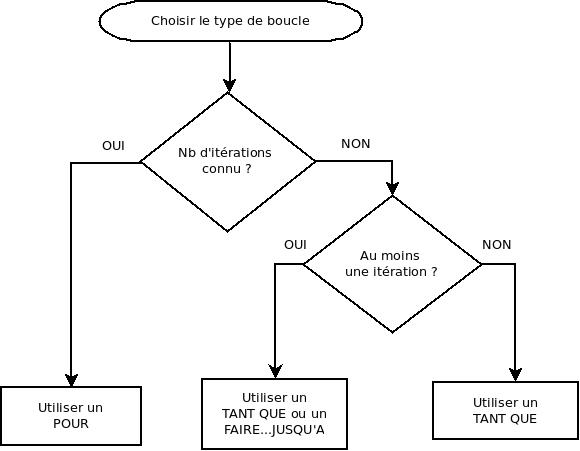
\includegraphics[width=.8\textwidth]{image/boucle-choixtype}
				\label{fig:boucle-choix}
	\end{center}

	
% ================================
\section{Acquisition de données multiples}
% ================================

	Il existe des problèmes
	où l'algorithme doit demander une série de valeurs
	à l'utilisateur pour pouvoir les traiter.
	Par exemple, les sommer, en faire la moyenne,
	calculer la plus grande\dots
	
	Dans ce genre de problème,
	on va devoir stocker chaque valeur donnée par l'utilisateur 
	dans une seule et même variable et la traiter avant de passer
	à la suivante.
	Prenons un exemple concret pour mieux comprendre.

	\begin{quote}
	On veut pouvoir calculer (et retourner)
	la somme d’une série de nombres donnés par l’utilisateur. 
	\end{quote}

	Il faut d’abord se demander 
	comment l’utilisateur va pouvoir indiquer
	combien de nombres il faut additionner 
	ou quand est-ce que le dernier nombre à additionner a été entré. 
	Voyons quelques possibilités.
	
	\clearpage
	\subsection{Variante 1 : nombre de valeurs connu} 
	%------------------------------------------------	
	
		L’utilisateur indique le nombre de termes au départ.
		Ce problème est proche de ce qui a déjà été fait.
		
		\begin{LDA}
		\LComment Lit des valeurs entières et retourne la somme des valeurs lues.
		\Algo{sommeNombres}{}{entier} \RComment Variante 1
			\Decl{nbValeurs}{entier} \RComment nb de valeurs à additionner
			\Decl{valeur}{entier} \RComment un des termes de l’addition
			\Decl{somme}{entier} \RComment la somme
			\Let somme \Gets 0 \RComment la somme se construit petit à petit. 0 au départ
			\Read nbValeurs
			\For{i}{1}{nbValeurs}
				\Read valeur
				\Let somme \Gets somme + valeur 
			\EndFor
			\Return somme
		\EndAlgo
		\end{LDA}

		\begin{Exercice}{Afficher les nombres impairs}
			Écrire un algorithme qui demande une série
			de valeurs entières à l'utilisateur
			et qui affiche celles qui sont impaires.
			L'algorithme commence par demander à l'utilisateur
			le nombre de valeurs qu'il désire donner.
		\end{Exercice}
			
	\subsection{Variante 2 : stop ou encore}
	%------------------------------------------------	
	
		Après chaque nombre, 
		on demande à l’utilisateur s’il y a encore un nombre à additionner.

		Ici, il faut chercher une solution différente
		car on ne connait pas au départ le nombre de valeurs à additionner et
		donc le nombre d’exécution de la boucle. On va devoir passer à un
		«~tant que~» ou un «faire - jusqu’à ce que». On peut
		envisager de demander en fin de boucle s’il reste
		encore un nombre à additionner. Ce qui donne~:

		\begin{LDA}
		\LComment Lit des valeurs entières et retourne la somme des valeurs lues.
		\Algo{sommeNombres}{}{entier} \RComment Variante 2a
			\Decl{encore}{booléen} \RComment est-ce qu’il reste encore une valeur à additionner~?
			\Decl{valeur}{entier} \RComment un des termes de l’addition
			\Decl{somme}{entier} \RComment la somme
			\Let somme \Gets 0
			\Repeat 
				\Read valeur
				\Let somme \Gets somme + valeur 
				\Read encore
			\EndRepeat{NON encore}
			\Return somme
		\EndAlgo
		\end{LDA}
		
		Avec cette solution, on additionne au moins une valeur. 
		Si on veut pouvoir tenir compte du
		cas très particulier où l’utilisateur ne veut
		additionner aucune valeur, il faut utiliser un «~tant que~» et donc
		poser la question avant d’entrer dans la boucle.

		\begin{LDA}
		\LComment Lit des valeurs entières et retourne la somme des valeurs lues.
		\Algo{sommeNombres}{}{entier} \RComment Variante 2b
			\Decl{encore}{booléen} \RComment est-ce qu’il reste encore une valeur à additionner~?
			\Decl{valeur}{entier} \RComment un des termes de l’addition
			\Decl{somme}{entier} \RComment la somme
			\Let somme \Gets 0
			\Read encore
			\While{encore} 
				\Read valeur
				\Let somme \Gets somme + valeur 
				\Read encore
			\EndWhile
			\Return somme
		\EndAlgo
		\end{LDA}

		\begin{Exercice}{Compter les nombres impairs}
			Écrire un algorithme qui demande une série
			de valeurs entières à l'utilisateur
			et qui lui affiche le nombre de valeurs impairs
			qu'il a donné.
			Après chaque valeur entrée,
			l'algorithme demande à l'utilisateur s'il y en a encore d'autres.
		\end{Exercice}

	\subsection{Variante 3 : valeur sentinelle}
		
		L’utilisateur entre une valeur spéciale pour indiquer la fin. 
		On parle de valeur \textbf{sentinelle}. 
		Ceci n’est possible que si cette valeur \textbf{sentinelle} ne peut pas être
		un terme valide de l’addition. Par exemple, si on veut
		additionner des nombres positifs uniquement, la valeur -1 peut servir
		de valeur sentinelle. Mais sans limite sur les nombres à additionner
		(positifs, négatifs ou nuls) il n’est pas possible de
		choisir une sentinelle.

		Ici, on se base sur la valeur entrée pour décider si on continue ou pas. 
		Il faut donc \textbf{toujours} effectuer un test
		après une lecture de valeur. C’est pour cela
		qu’il faut effectuer une lecture avant et une autre à
		la fin de la boucle.

		\begin{LDA}
		\LComment Lit des valeurs entières et retourne la somme des valeurs lues.
		\Algo{sommeNombres}{}{entier} \RComment Variante 3
			\Decl{valeur}{entier} \RComment un des termes de l’addition
			\Decl{somme}{entier} \RComment la somme
			\Let somme \Gets 0
			\Read valeur
			\While{valeur ${\geq}$ 0} 
				\Let somme \Gets somme + valeur 
				\Read valeur \RComment remarquer l’endroit où on lit une valeur.
			\EndWhile
			\Return somme
		\EndAlgo
		\end{LDA}

		\begin{Exercice}{Choix de la valeur sentinelle}
			Quelle valeur sentinelle prendrait-on 
			pour additionner une série de cotes d’interrogations~? 
			Une série de températures~?
		\end{Exercice}

		\begin{Exercice}{Afficher les nombres impairs}
			Écrire un algorithme qui demande une série
			de valeurs entières non nulles à l'utilisateur
			et qui affiche celles qui sont impaires
			La fin des données sera signalée 
			par la valeur sentinelle 0.
		\end{Exercice}

		\begin{Exercice}{Compter le nombre de réussites}
			Écrire un algorithme qui demande une série
			de cotes (entières, sur 20) à l'utilisateur
			et qui affiche le pourcentage de réussites.
			La fin des données sera signalée 
			par une valeur sentinelle que vous pouvez choisir.
		\end{Exercice}


% ================================
\section{Les suites}
% ================================

	Nous avons vu quelques exemples d'algorithmes
	qui affichent une suite de nombres
	(par exemple, afficher les nombres pairs).
	Nous avons pu les résoudre facilement
	avec un \lda{\algorithmicfor}
	en choisissant judicieusement les valeurs de début et de fin
	ainsi que le pas.
	
	Ce n'est pas toujours aussi simple.
	Nous allons voir deux exemples plus complexes
	et les solutions qui vont avec.
	Elles pourront se généraliser à beaucoup d'autres exemples.
	
	\subsubsection{Exemple - Afficher les carrés}
	%--------------------------------------------
	
		On veut afficher les $n$ premiers nombres carrés parfaits :
		$1$, $4$, $9$, $16$, $25$\dots

		Si on vous demande : "Quel est le 7\ieme{} nombre à afficher ?".
		Vous répondrez : "Facile ! C'est $7^2$, soit $49$".
		Plus généralement, le nombre à afficher 
		lors du $i$\ieme{} passage dans la boucle est $i^2$.

		\begin{tabular}{l|*{8}{>{\centering\arraybackslash}m{8mm}}}
		 étape & 1 & 2 & 3 & 4 & 5 & 6 & 7 & 8\\\hline
		 valeur à afficher & 1 & 4 & 9 & 16 & 25 & 36 & 49 & 64 \\
		\end{tabular}
		
		L'algorithme qui en découle est :
		
		\begin{LDA}
			\Algo{suiteCarrés}{\Par{n}{entier}}{}
				\For{i}{1}{n}
					\Write $i^2$
				\EndFor
			\EndAlgo
		\end{LDA}

		Dans cette solution,
		la variable de contrôle compte simplement le nombre d’itérations.
		On calcule le nombre à afficher en fonction cette variable de contrôle 
		(ici le carré convient).
		Par une vieille habitude des programmeurs%
		\footnote{%
			Née avec le langage FORTRAN 
			où la variable $i$ était par défaut une variable entière.
		},
		une variable de contrôle 
		qui se contente de compter les passages dans la boucle 
		est souvent nommée $i$. 
		On l’appelle aussi «~itérateur~».	

		Cette solution peut être utilisée
		chaque fois qu'on peut calculer le nombre à afficher
		en fonction de $i$.
		
	\subsubsection{Exemple - Une suite un peu plus complexe}
	%-------------------------------------------------------
	 
		Écrire un algorithme qui affiche 
		les $n$ premiers nombres de la suite :
		1, 2, 4, 7, 11, 16\dots{}
		
		Comme on peut le constater, 
		à chaque étape on ajoute un peu plus au nombre précédent.
		\[ 
			1 
			\xrightarrow{+1} 2 
			\xrightarrow{+2} 4
			\xrightarrow{+3} 7 
			\xrightarrow{+4} 11 
			\xrightarrow{+5} 16 
			\dots
		\] 

		Ici, difficile de partir de la solution de l'exemple précédent
		car il est n'est pas facile de trouver la fonction $f(i)$
		qui permet de calculer le nombre à afficher en fonction de i. 
		
		Par contre, il est assez simple de calculer ce nombre 
		en fonction du précédent.
		\[
			\mbox{nb à afficher} = \mbox{nb affiché juste avant} + i
		\]
		Sauf pour le premier, qui ne peut pas être calculé
		en fonction du précédent.
		Une solution élégante et facilement adaptable
		à d'autres situations est :
		
		\begin{LDA}
			\Algo{suite}{\Par{n}{entier}}{}
				\Decl{val}{entier}
				\Let val \Gets \textit{1\iere{} valeur à afficher}
				\For{i}{1}{n}
					\Write val
					\Let val \Gets \textit{la valeur suivante calculée à partir de la valeur courante}
				\EndFor
			\EndAlgo
		\end{LDA}
		
		qui, dans notre exemple précis, devient :

		\begin{LDA}
			\Algo{suite}{\Par{n}{entier}}{}
				\Decl{val}{entier}
				\Let val \Gets 1
				\For{i}{1}{n}
					\Write val
					\Let val \Gets val + i
				\EndFor
			\EndAlgo
		\end{LDA}

	\subsubsection{Exercices}
	%-------------------------------------------------------
		
		\begin{Exercice}{Suites}
			Écrire les algorithmes qui affichent
			les $n$ premiers termes des suites suivantes.
			À vous de voir quel est le canevas de solution
			le plus adapté.
			\begin{enumerate}[label=\alph*)]
			\item -1, -2, -3, -4, -5, -6\dots
			\item 1, 3, 6, 10, 15, 21, 28\dots
			\item 1, 0, 1, 0, 1, 0, 1, 0\dots
			\item 1, 2, 0, 1, 2, 0, 1, 2\dots
			\item 1, 2, 3, 1, 2, 3, 1, 2\dots
			\item 1, 2, 3, 2, 1, 2, 3, 2\dots
			\end{enumerate}			
		\end{Exercice}
				
% ================================
\section{Exercices récapitulatifs}
% ================================

	\begin{Exercice}{Lire un nombre}
		Écrire un algorithme 
		qui demande à l'utilisateur un nombre entre 1 et $n$
		et le retourne.
		Si la valeur donnée n'est pas dans l'intervalle souhaité,
		l'utilisateur est invité à rentrer une nouvelle valeur
		jusqu'à ce qu'elle soit correcte.
		\begin{LDA}
			\Entete{lireNb}{\Par{n}{entier}}{entier}
		\end{LDA}
		
		\paragraph{Solution.}
		Si la valeur donnée par l'utilisateur était toujours
		correcte, il suffirait d'écrire :
		\begin{LDA}
			\Algo{lireNb}{\Par{n}{entier}}{entier}
				\Decl{val}{entier}
				\Read{val}
				\Return val
			\EndAlgo
		\end{LDA}
		Pour tenir compte des entrées invalides, 
		il faut ajouter une boucle qui
		prévient que la valeur est mauvaise et la redemande.
		Et ceci, tant que c'est incorrect. 
		Ce qui donne :
		\begin{LDA}
			\Algo{lireNb}{\Par{n}{entier}}{entier}
				\Decl{val}{entier}
				\Read{val}
				\While{val<1 OU val>n}
					\Write "valeur incorrecte"
					\Read{val}
				\EndWhile
				\Return val
			\EndAlgo
		\end{LDA}
		La solution qu'on obtient est proche d'une lecture répétée
		avec valeur sentinelle.
		Dans ce cas, la valeur sentinelle est toute valeur correcte.
	\end{Exercice}

	\begin{Exercice}{Lancé de dés}
		Écrire un algorithme qui lance $n$ fois un dé
		et compte le nombre de fois qu'une certaine valeur est obtenue.
		\begin{LDA}
			\Entete{lancerDé}{\Par{n}{entier}, \Par{val}{entier}}{entier}
		\end{LDA}
	\end{Exercice}
	
	\begin{Exercice}{Factorielle}
		Écrire un algorithme qui retourne la factorielle de $n$ (entier positif ou
		nul). Rappel~: la factorielle de $n$, notée $n$!, est le produit des $n$
		premiers entiers strictement positifs. 
		
		Par convention, 0! = 1.
	\end{Exercice}

	\begin{Exercice}{Produit de 2 nombres}
		Écrire un algorithme qui retourne le produit de deux entiers quelconques
		sans utiliser l’opérateur de multiplication, mais en minimisant le
		nombre d’opérations.
	\end{Exercice}

	\begin{Exercice}{Table de multiplication}

		\begin{minipage}[t]{10cm}
			Écrire un algorithme qui affiche la table de multiplication
			des nombres de 1 à 10
			(cf. l'exemple ci-contre).

			\medskip
			Attention ! Nous somme en algorithmique, 
			ne vous préoccupez pas de la mise en page de ce qui est affiché.
			Ce sera une question importante quand vous traduirez 
			l'algorithme dans un langage de programmation mais pas ici. 
		\end{minipage}
		\qquad
		\begin{minipage}[t]{4cm}
		\begin{verbatim}
			1 x 1 = 1
			1 x 2 = 2
			...
			1 x 10 = 10
			2 x 1 = 2
			...
			10 x 9 = 90
			10 x 10 = 100
		\end{verbatim}
		\end{minipage}		
	\end{Exercice}
	
	\begin{Exercice}{Double 6}
		Écrire un algorithme qui lance de façon répétée deux dés.
		Il s'arrête lorsqu'il obtient un double 6
		et retourne le nombre de lancés effectués.
	\end{Exercice}
	
	\begin{Exercice}{Nombre premier}
		Écrire un algorithme qui vérifie si un entier positif est un
		\textbf{nombre premier}. 
		
		Rappel~:~un nombre est premier s’il n’est divisible que par 1 et par
		lui-même. Le premier nombre premier est 2.
	\end{Exercice}
	
	\begin{Exercice}{Nombres premiers}
		Écrire un algorithme qui affiche les nombres premiers inférieurs ou
		égaux à un entier positif donné. Le module de cet algorithme fera appel
		de manière répétée mais économique à celui de l’exercice précédent.
	\end{Exercice}

	\begin{Exercice}{Somme de chiffres}
		\marginicon{java}
		Écrire un algorithme qui calcule la somme des chiffres qui forment un
		nombre naturel $n$. Attention, on donne au départ \textbf{le} nombre et
		pas ses chiffres. Exemple~: 133045 doit donner comme résultat 16,
		car 1 + 3 + 3 + 0 + 4 + 5 = 16.
	\end{Exercice}
	
	\begin{Exercice}{Nombre parfait}
		Écrire un algorithme qui vérifie si un entier positif est un
		\textbf{nombre parfait}, c’est-à-dire un nombre égal à la somme de ses
		diviseurs (sauf lui-même). 
		
		Par exemple, 6 est parfait car 6 = 1 + 2 + 3. 
		De même, 28 est parfait car 28 = 1 + 2 + 4 + 7 + 14.
	\end{Exercice}
	
	\begin{Exercice}{Décomposition en facteurs premiers}
		Écrire un algorithme qui affiche la décomposition 
		d’un entier en facteurs premiers. 
		Par exemple, $1001880$ donnerait comme décomposition
		$2^3 * 3^2 * 5 * 11^2 * 23$.
	\end{Exercice}

	\begin{Exercice}{Nombre miroir}
		Le miroir d'un nombre est le nombre obtenu
		en lisant les chiffres de droite à gauche.
		Ainsi le nombre miroir de $4209$ est $9024$.
		Écrire un algorithme qui calcule le miroir
		d'un nombre entier positif donné.
	\end{Exercice}
	
	\begin{Exercice}{Palindrome}
		Écrire un algorithme qui vérifie si un entier donné 
		forme un palindrome ou non. 
		Un nombre palindrome est un nombre qui lu dans un sens 
		(de gauche à droite) est identique au nombre lu dans l’autre sens 
		(de droite à gauche). 
		Par exemple, $1047401$ est un nombre palindrome.
	\end{Exercice}
	
	\begin{Exercice}{Jeu de la fourchette}
		\marginicon{java}
		Écrire un algorithme qui simule le jeu de la
		fourchette. Ce jeu consiste à essayer de découvrir un nombre quelconque
		compris entre 1 et 100 inclus, tiré au sort par l’ordinateur (la primitive
		\lda{hasard(n~:~entier)} retourne un entier entre 1 et $n$). 
		L’utilisateur a droit à huit essais
		maximum. À chaque essai, l’algorithme devra afficher un message
		indicatif «~nombre donné trop petit~» ou «~nombre donné trop grand~».
		En conclusion, soit «~bravo, vous avez trouvé en [nombre] essai(s)~» soit
		«~désolé, le nombre était [valeur]~».
	\end{Exercice}
	

		\chapter{Les tableaux}
			\begin{Note}
				Pour éviter que de trop nombreux étudiants
				se plantent dans la traduction en Java,
				on va utiliser le plus souvent des tableaux
				qui commencent à 0.
				
				(mcd:) j'ai en tête une notation qui sera simple
				et facile pour des tableaux commençant à 0
				mais permettrait d'avoir aussi des tableaux
				commençant à 1 si on veut faire un ou deux exercices
				là-dessus. Coming soon\dots 
			\end{Note}
			
			\begin{TODO}
				\begin{itemize}
				\item
					Récupérer toute l'introduction théorique
					du syllabus de cette année.
				\item
					Enlever tout ce qui sera traité dans la partie
					"Algorithmes fondamentaux".
				\item
					Commencer par des exercices simples de parcours.
				\item
					Voir si c'est ici qu'on introduit la complexité.
				\end{itemize}
			\end{TODO}

	\part{Les algorithmes fondamentaux}
	%----------------------------------------------------------
		\chapter{Agrégation des données}
			\begin{Note}
			On va retrouver ici tout ce qui concerne l'agrégation
			de données, d'un tableau essentiellement
			\begin{itemize}
			\item somme, moyenne\dots
			\item recherche de maximum/minimum
			\item indices du maximum/minimum
			\item \dots
			\end{itemize}
			\end{Note}
		\chapter{Recherche de valeurs}
			\begin{Note}
			On va retrouver ici tout ce qui concerne la recherche
			de valeur dans un tableau, trié ou pas.
			\end{Note}
		\chapter{Tris}
			\begin{Note}
			On va retrouver ici,
			peu ou prou le chapitre actuel sur les tris.
			\end{Note}
		\chapter{Acquisition des données}
			\begin{Note}
			On va retrouver ici tout ce qui concerne la lecture
			de données multiples (avec valeur sentinelle).
			\end{Note}
		\chapter{Les suites}
			\begin{Note}
			On va retrouver ici tout ce qui concerne la génération 
			de suites.
			\end{Note}
	
	\part{Compléments}
	%----------------------------------------------------------
		\chapter{Les chaines}
			\begin{Note}
			Traiter ici de la manipulation des chaines.
			Cf. le syllabus de cette année
			qu'il faudra peut-être adapter.
			\end{Note}
		\chapter{Les structures}
			\begin{Note}
			Les structures sont une préparation aux cours
			du second quadrimestre
			\begin{itemize}
			\item l'OO en java
			\item les fichiers structurés en persistance des données
			\item les données structurées en Cobol
			\end{itemize}
			\end{Note}

	\appendix
	%----------------------------------------------------------
	
	\part{Les annexes}
		\chapter{Les fiches}

Vous trouverez ici toutes les fiches
des algorithmes analysés dans ce cours.

\vspace*{-3cm}
\listoffiche
%\printcontents[fiches]{}{0}{\setcounter{tocdepth}{1}}

%\startcontents[fiches]
\cleardoublepage\begin{Fiche}{Un calcul simple}
\label{fiche:calcul-simple}

\Section{Le problème}
	Calculer la surface d'un rectangle 
	à partir de sa longueur et sa largeur.

\Section{Spécification}

	\paragraph{Données}
	\begin{itemize}
	\item La longueur du rectangle ;
	\item sa largeur.
	\end{itemize}
	Toutes les données sont des réels positifs ou nuls.

	\paragraph{Résultat.}
	Un réel représentant la surface du rectangle

	\bigskip
	\begin{center}	
	\flowalgodd{longueur (réel)}{largeur (réel)}{surfaceRectangle}{réel}
	\end{center}

\Section{Exemples}

	\begin{itemize}
	\item \lda{surfaceRectangle(4, 3)} donne $12$
	\item \lda{surfaceRectangle(2.5, 2)} donne $5$
	\end{itemize}

\Section{Analyse de la solution}

	La surface d'un rectangle est obtenue en multipliant
	la largeur par la longueur.
	\begin{equation}
		\textrm{surface} = \textrm{longueur} * \textrm{largeur}
	\end{equation}
	
\Section{Solution}

	\begin{LDA}
	%\LComment Calcule la surface du rectangle
	%\LComment Données : la longueur et la largeur du rectangle
	%\LComment Résultat : la surface du rectangle
	%mcd: je trouve çà un peu bateau à ce stade
	\Algo{surfaceRectangle}{\Par{longueur, largeur}{réel}}{réel}
		\Return longueur * largeur
	\EndAlgo
	\end{LDA}

\Section{Quand l'utiliser ?}

	Ce type de solution peut être utilisé à chaque fois
	que la réponse s'obtient par un calcul simple sur les données.
	Si le calcul est plus complexe, 
	il peut être utile de le décomposer pour accroitre la lisibilité
	(cf. fiche \vref{fiche:calcul-complexe}) 
	
\end{Fiche}

\cleardoublepage\begin{Fiche}{Un calcul complexe}
\label{fiche:calcul-complexe}

\Section{Le problème}
	Calculer la vitesse (en km/h) d'un véhicule dont on donne
	la durée du parcours (en secondes) 
	et la distance parcourue (en mètres).

\Section{Spécification}

	\paragraph{Données}
	\begin{itemize}
	\item la distance parcourue par le véhicule (en m);
	\item la durée du parcours (en s).
	\end{itemize}
	Toutes les données sont des réels

	\paragraph{Résultat.}
	Un réel représentant la vitesse du véhicule (en km/h).

	\bigskip
	\begin{center}	
	\flowalgodd{distanceM (réel)}{duréeS (réel)}{vitesseKMH}{réel}
	\end{center}

\Section{Exemples}

	\begin{itemize}
	\item \lda{vitesseKMH(100,10)} donne $36$
	\item \lda{vitesseKMH(10000,3600)} donne $10$
	\end{itemize}

\Section{Analyse de la solution}

	La vitesse est liée à la distance et à la durée par la formule :
	\begin{equation}
		\textrm{vitesse} = \frac{\textrm{distance}}{\textrm{durée}}
	\end{equation}

	pour autant que les unités soient cohérentes.
	Ainsi pour obtenir une vitesse en km/h, 
	il faut convertir la distance en kilomètres 
	et la durée en heures.
		
\Section{Solution}

	\begin{LDA}
%	\LComment Calcule la vitesse d'un véhicule en connaissant la distance et la durée
%	\LComment Données : la distance parcourue en m et le temps écoulé en secondes
%	\LComment Résultat : la vitesse du véhicule en km/h
	\Algo{vitesseKMH}{\Par{distanceM, duréeS}{réel}}{réel}
		\Decl{distanceKM, duréeH}{réel}
		\Let distanceKM \Gets $\frac{\textrm{distanceM}}{1000}$
		\Let duréeH \Gets $\frac{\textrm{duréeS}}{3600}$
		\Return $\frac{\textrm{distanceKM}}{\textrm{duréeH}}$
	\EndAlgo
	\end{LDA}

\Section{Quand l'utiliser ?}

	Ce type de solution peut être utilisé à chaque fois
	que la réponse s'obtient par un calcul complexe sur les données
	qu'il est bon de décomposer pour aider à sa lecture.
	Si le calcul est plutôt simple, 
	on peut le garder en une seule assignation
	(cf. fiche \vref{fiche:calcul-simple}).
	
\end{Fiche}

\cleardoublepage\begin{Fiche}{Un nombre (im)pair}
\label{fiche:calcul-pair}

\Section{Le problème}
	Un nombre reçu en paramètre est-il pair~?

\Section{Analyse}

	Un nombre est pair si il est multiple de 2. 
	C'est-à-dire si le reste de sa division par 2 vaut 0.
	\begin{LDA}
		\Stmt estPair est vrai si nombre MOD 2 = 0
	\end{LDA}

	\paragraph{Données}
	\begin{itemize}
	\item le nombre entier dont on veut savoir si il est pair.
	\end{itemize}

	\paragraph{Résultat.}
	Un booléen à \textit{vrai} si le \textit{nombre} est pair et \textit{faux} sinon.

	\bigskip
	\begin{center}	
	\SchemaModulei{nombre (entier)}{isPair}{booléen}
	\end{center}

\Section{Exemples}

	\begin{itemize}
	\item \lda{isPair(2016)} donne $vrai$
	\item \lda{isPair(2015)} donne $faux$
	\end{itemize}
	
\Section{Solution}

	\begin{LDA}
%	\LComment Retourne vrai si le nombre reçu en paramètre est pair et faux sinon.
%	\LComment Données : le nombre dont on veut savoir si il est pair
%	\LComment Résultat : vrai si le nombre est pair et faux sinon.
	\Algo{isPair}{\Par{nombre}{entier}}{booléen}
		\Return nombre MOD 2 = 0
	\EndAlgo
	\end{LDA}

\Section{Alternatives}

	\begin{minipage}{7.5cm}
		\begin{LDA}
		\Algo{isPair}{\Par{nombre}{entier}}{booléen}
			\If{nombre MOD 2 = 0}
				\Return vrai
			\Else
				\Return faux
			\EndIf
		\EndAlgo
		\end{LDA}
	\end{minipage}
	\quad
	\begin{minipage}{6cm}
		Certains étudiants se sentent plus à l'aise avec
		la solution ci-contre en début d'année.			
		C'est probablement parce qu'elle colle plus à la façon de l'exprimer
		en français.
		On les encourage toutefois à rapidement 
		passer à la version plus compacte
		et, une fois habitué, plus lisible.
	\end{minipage}

	\hfil\rule{0.5\textwidth}{.4pt}\hfil

	\begin{minipage}{7.5cm}
		\begin{LDA}
		\Algo{isPair}{\Par{nombre}{entier}}{booléen}
			\If{nombre MOD 2 = 0}
				\Return vrai
			\EndIf
			\Return faux
		\EndAlgo
		\end{LDA}
	\end{minipage}
	\quad
	\begin{minipage}{6cm}
		On rencontre également ce genre de solution
		qui, pour certains, 
		parait mieux que la précédente 
		parce qu'elle ne contient pas de "sinon"
		et est donc plus courte.
		Il n'en n'est rien.
		Rappelons que la longueur de l'algorithme
		n'est pas, en soi, un critère de qualité. 
	\end{minipage}
	
\Section{Quand l'utiliser ?}

	À chaque fois qu'un résultat booléen dépend d'un calcul simple.
	Si le calcul est plus compliqué, on peut le décomposer comme
	indiqué dans la fiche \vref{fiche:calcul-complexe}.
	
	On peut également s'inspirer de cette solution
	quand il faut donner sa valeur à une variable booléenne.
		
\end{Fiche}
		
\cleardoublepage%======================================
\begin{Fiche}{Maximum de deux nombres}
%======================================
\label{fiche:max2nb}

	Quel est le maximum de deux nombres ?

\Section{Analyse}

	Voilà un classique de l'algorithmique.
	Attention ! On ne veut pas savoir \emph{lequel}
	est le plus grand mais juste la valeur.
	Il n'y a donc pas d'ambigüité si les deux nombres sont égaux.

	\textbf{Données} : deux nombres réels.
		
	\textbf{Résultat} : un réel contenant la plus grande des deux valeurs données.

	\begin{center}	
		\flowalgodd{nb1 (réel)}{nb2 (réel)}{max2}{réel}
	\end{center}

\Section{Exemples}

	\vspace*{-3mm}
	\begin{multicols}{3}
		\begin{itemize}
		\item \lda{max2(-3, 4)} donne $4$
		\item \lda{max2(7, 4)} donne $7$
		\item \lda{max2(4, 4)} donne $4$
		\end{itemize}
	\end{multicols}
	\vspace*{-6mm}
	
\Section{Solution}

	\begin{LDA}
	\Algo{max2}{\Par{nb1}{réel}, \Par{nb2}{réel}}{réel}
		\Decl{max}{réel}
		\If{nb1 > nb2}
			\Let max \Gets nb1
		\Else
			\Let max \Gets nb2
		\EndIf
		\Return max
	\EndAlgo
	\end{LDA}

\Section{Alternatives}

	\begin{minipage}{7.0cm}
		\begin{LDA}
		\Algo{max2}{\Par{nb1}{réel}, \Par{nb2}{réel}}{réel}
			\If{nb1 > nb2}
				\Return nb1
			\Else
				\Return nb2
			\EndIf
		\EndAlgo
		\end{LDA}
	\end{minipage}
	\quad
	\begin{minipage}{6.5cm}
		En algorithmique, comme ailleurs, il existe des modes.
		Certaines personnes insistent pour qu'il n'y ait qu'un seul
		retour en fin d'algorithme ; 
		d'autres admettent un retour à la fin de chaque
		branche de l'alternative.
		En début d'apprentissage,
		on vous demande de n'utiliser qu'un seul retour
		pour éviter tout abus.
	\end{minipage}

	\hfil\rule{0.5\textwidth}{.4pt}\hfil

	\begin{minipage}{7.0cm}
		\begin{LDA}
		\Algo{max2}{\Par{nb1}{réel}, \Par{nb2}{réel}}{réel}
			\Decl{max}{réel}
			\Let max \Gets nb1
			\If{nb2 > nb1}
				\Let max \Gets nb2
			\EndIf
			\Return max
		\EndAlgo
		\end{LDA}
	\end{minipage}
	\quad
	\begin{minipage}{6.5cm}
		Certains écrivent parfois une solution de ce genre
		mais ne la défendent pas avec les bons arguments.
		Le fait de ne pas avoir de "sinon" n'est absolument pas pertinent.
		Son avantage est qu'elle se généralise plus facilement
		au cas où il y a plusieurs nombres dont on veut le maximum.
		Pour deux nombres, on lui préférera la solution proposée plus haut.
	\end{minipage}
	
\Section{Quand l'utiliser ?}

	Cet algorithme peut bien sûr être facilement adapté
	à la recherche du minimum.
		
\end{Fiche}
		
%\stopcontents[fiches]

		\chapter{Le LDA}

	Dans cette annexe nous définissons le LDA
	(\emph{le Langage de Description d'Algorithmes})
	que nous allons utiliser. 
	Nous ne nous attarderons pas sur les concepts
	ni sur certaines bonnes pratiques;
	tout cela est vu dans les chapitres associés.
	
	Nous utilisons un pseudo-code pour nous libérer 
	des contraintes des langages de programmation.
	\begin{itemize}
	\item
		Un programme est une suite de lignes
		ne permettant pas d'utiliser pleinement les
		deux dimensions de la page 
		(pensons à la mise en page des formules).
	\item
		Certaines constructions et règles
		n'existent que pour simplifier le travail du compilateur
		et/ou accélérer le code.
		C'est le cas, par exemple, de la syntaxe du \emph{switch}.
	\end{itemize}
	
	Dans vos réflexions, brouillons, premiers jets,
	nous vous encourageons à utiliser des notations
	qui vous sont propres et qui vous permettent
	de poser votre réflexion sur un papier
	et d'avancer vers une solution.
	
	La version finale, toutefois, 
	doit être lue par d'autres personnes.
	Il est \textbf{essentiel} qu'il n'y ait aucune ambigüité
	sur le sens de votre écrit.
	C'est pourquoi, nous devons définir une notation
	à la fois souple et précise.
	
	Cette notation doit aussi être adaptée à des étudiants de première année.
	Ce qui nous amène à ne pas introduire des nuances qui leur échappent encore
	et, parfois, à imposer des contraintes qui seront relâchées plus tard
	mais qui permettent de cadrer l'apprentissage d'un débutant.
	
	\textbf{Remarque} : Ce guide n'est pas universel.
	En dehors de l'école, d'autres notations sont utilisées,
	parfois proches, parfois plus lointaines.
	Votre professeur pourra également introduire quelques notations
	qui ne sont pas reprises ici 
	ou relâcher quelques contraintes définies ici. 
	Lorsque vous changerez de professeur,
	soyez conscient que ces ajouts ne seront peut-être plus valables.
	
	L'important est que le groupe qui doit communiquer
	au moyen d'algorithmes se soit préalablement mis d'accord 
	sur des notations.

\subsection*{Un algorithme}
%---------------------------------

	\begin{minipage}{6cm}
		\begin{LDA}
			\Algo{nom}{paramètres}{Type}
				\Stmt Instructions
				\Return expression
			\EndAlgo
		\end{LDA}
	\end{minipage}
	\qquad
	\begin{minipage}{6cm}
		\begin{LDA}
			\Algo{nom}{paramètres}{}
				\Stmt Instructions
			\EndAlgo
		\end{LDA}
	\end{minipage}

	On permet l'utilisation du raccourci \lda{\K{algo}}.
	
\subsection*{Types, variables et constantes}
%-----------------------------------

	Les types permis sont :
	\lda{entier}, \lda{réel},
	\lda{booléen} et \lda{chaine}.

	\begin{LDA}
		\Const{nom}{valeur}
		\Decl{var1, \dots}{Type} 
	\end{LDA}

\subsection*{Les instructions de base}
%---------------------------------

	\begin{LDA}
		\Let var \Gets expression
		\Read var1, var2\dots
		\Write expression1, expression2\dots
		\Error "raison" \Comment Provoque l'arrêt de l'algorithme.
	\end{LDA}
	
\subsection*{Les instructions de choix}
%---------------------------------

	\begin{minipage}[t]{4.5cm}
	\begin{LDA}
	\If{condition}
		\Stmt Instructions
	\EndIf
	\Empty
	\Empty
	\Empty
	\Empty
	\Empty
	\Empty
	\end{LDA}
	\end{minipage}
	\ 
	\begin{minipage}[t]{4.5cm}
	\begin{LDA}
	\If{condition}
		\Stmt Instructions
	\Else
		\Stmt Instructions
	\EndIf
	\Empty
	\Empty
	\Empty
	\Empty
	\end{LDA}
	\end{minipage}
	\ 
	\begin{minipage}[t]{4.5cm}
	\begin{LDA}
	\If{condition}
		\Stmt Instructions
	\ElsIf{condition}
		\Stmt Instructions
	\ElsIf{condition}
		\Stmt \dots
	\Else
		\Stmt Instructions
	\EndIf
	\end{LDA}
	\end{minipage}
	
	\begin{LDA}
		\Switch{expression}
			\Case{liste${}_1$ de valeurs séparées par des virgules }
				\Stmt Instructions
			\Case{liste${}_2$ de valeurs séparées par des virgules }
				\Stmt Instructions
			\Empty \dots
			\Case{liste${}_k$ de valeurs séparées par des virgules }
				\Stmt Instructions
			\Case{\K{autres }}
				\Stmt Instructions
		\EndSwitch
	\end{LDA}
	
	où l'expression peut être de type \lda{entier} ou \lda{chaine}
	(pas de \lda{réel}) et les valeurs sont des constantes.

\subsection*{Les instructions de répétition}
%---------------------------------

	\begin{minipage}[t]{4cm}	
	\begin{LDA}
		\While{condition}
			\Stmt Instructions
		\EndWhile
	\end{LDA}
	\end{minipage}
	\
	\begin{minipage}[t]{6.5cm}	
	\begin{LDA}
		\For[pas]{indice}{début}{fin}
			\Stmt Instructions
		\EndFor
	\end{LDA}
	\end{minipage}
	\
	\begin{minipage}[t]{4cm}	
	\begin{LDA}
		\Repeat
			\Stmt Instructions
		\EndRepeat{condition}
	\end{LDA}
	\end{minipage}
	
	\begin{itemize}
	\item
		La boucle \lda{pour} ne peut être utilisée que pour des entiers.
	\item
		Le \lda{\K{par} pas} peut être omis si le pas vaut 1.
	\item
		Il n'est \textbf{pas nécessaire} de déclarer l'indice.
		Il ne peut être utilisé en dehors de la boucle et ne peut pas
		être modifié à l'intérieur de la boucle.
		De même, le \lda{début}, la \lda{fin} et le \lda{pas} 
		ne peuvent pas être modifiés dans la boucle.
	\end{itemize}
	

	
	% =======================================================
% Table des matières
% =======================================================

\printindex
\addcontentsline{toc}{chapter}{Index}



\end{document}
